%%% Main LaTeX file for the diaspora-srd project.
%%%
%%% This file is distributed under the Artistic Licence, v.2.0
%%% You should have received a file containing the license along
%%% with this file; if not see:
%%% http://www.perlfoundation.org/artistic_license_2_0
%%%
%%% TODO simplify producing different page formats
%%%   landscape/portrait ; letterpaper/a4paper
\documentclass[10pt,twocolumn,landscape,letterpaper]{memoir}
% \documentclass[10pt,twocolumn,landscape,letterpaper]{rpgrulebook}
% This file was converted from HTML to LaTeX with
% Tomasz Wegrzanowski's <maniek@beer.com> gnuhtml2latex program
% \documentclass[onecolumn]{memoir}
% \documentclass[twocolumn]{memoir}
% \documentclass[10pt,twocolumn,letterpaper]{rpgrulebook}
% \documentclass[10pt,onecolumn,letterpaper]{rpgrulebook}
% \documentclass[10pt,onecolumn,landscape,letterpaper]{rpgrulebook}

\usepackage{diaspora-srd} % customizations

\title{Diaspora SRD}
\author{
Authors:
Brad Murray, C.W. Marshall, Tim Dyke, Byron Kerr \\
Typesetting:
% \href{mailto:wagener+diaspora@gmail.com}
{Harald Wagener}
\\
Layout:
% \href{mailto:nick@zork.net}
{Nick Moffitt},
{Harald Wagener}
\\
\LaTeX{} version: {David Leaman}
}
\date{}


% TODO: complete index
\makeindex
% TODO: create glossary
% \makeglossary

\begin{document}

\frontmatter
\maketitle

\footnoterule
% TODO bottom-align this
% \footnotetext{
This file version \VERSION

Diaspora is \copyright~\href{http://www.vsca.ca/Diaspora}{VSCA Publishing}
% }

\tableofcontents
\listoftables
\mainmatter

%%% ``Playing With FATE'' chapter of the Diaspora SRD
%%%
%%% This file is distributed under the Artistic Licence, v.2.0
%%% You should have received a file containing the license along
%%% with this file; if not see:
%%% http://www.perlfoundation.org/artistic_license_2_0
%%%
\chapter{Playing with FATE}
\label{cha:playing-with-fate}

Diaspora is a role-playing game with a focus on hard(ish) science-fiction adventure. You build a universe, you build characters, and then you play with them in it.

Underpinning the game is the task resolution system described in this chapter.

\index{Spirit of the Century}
All conflicts in Diaspora are resolved using the FATE mechanics as elaborated in \emph{Spirit of the Century} and available from the System Reference Document for that game, available on the \href{http://bzr.mausdompteur.de/fate3/fate3.html}{Internet}.%
\footnote{ \texttt{http://bzr.mausdompteur.de/fate3/fate3.html} }

You roll your set of four fudge dice, which yields a result between -4 and +4, you add an appropriate skill, and then you compare against some difficulty level, which might be someone else's roll or might be a level imposed by the referee.

%%% Define some text blocks, and then lay them out depending on the
%%% document layout.
%
%% blurb about fudge dice
\def\FUDGEDICE{
\index{dice!fudge dice}
Almost every roll in \emph{Diaspora} is \dF: a single roll of four Fudge dice, yielding a range from -4 to +4. A Fudge die is a d6, with two faces marked -, two marked +, and two blank. You add up the +s, subtract the -s, and you have a total.
The resultant probability curve is the same as rolling \texttt{4d3-8}, so you could use ordinary \texttt{d6}s and treat 1--2 as -, 3--4 as blank, and 5--6 as +.
}%
%
%% blurb about alternate dice systems
\def\ALTDICE{
\index{dice!alternate systems}
{\medskip\large\bfseries Option: alternate dice systems}
%
% The system will work with a different probability curve by using one of the following die mechanics:
\begin{description}
\item [\texttt{d6-d6}, $\pm5$]
Roll two different-coloured six-sided dice and subtract one from the other. You can establish whatever convention you like for which die is which (such as subtracting dark from light, or red from black), as long as you are consistent.

\item [\texttt{d6-d6}, $\pm4$]
As above, but treat $\pm5$ as 0. This has the same numeric range as \dF, but with a better chance of an extreme result.
\end{description}
}%
%
%% probability comparison table
\def\DICETABLE{
\begin{tabular}{r@{}l*3{r@{/}lr@{.}l}}
\multicolumn{2}{c}{}
{}	& \multicolumn{4}{c}{\dF}
{}	& \multicolumn{4}{c}{\texttt{d6-d6}, $\pm4$}
{}	& \multicolumn{4}{c}{\texttt{d6-d6}, $\pm5$} \\
\toprule
\multicolumn{2}{c}{roll}
{}	& \multicolumn{2}{c}{odds} & \multicolumn{2}{c}{\%}
{}	& \multicolumn{2}{c}{odds} & \multicolumn{2}{c}{\%}
{}	& \multicolumn{2}{c}{odds} & \multicolumn{2}{c}{\%} \\
\midrule
$\pm$&5	& \multicolumn{8}{c}{}		&  1&36	&  2&77 \\
$\pm$&4	&  1&81	&  1&24	&  2&36	&  5&55	&  2&36	&  5&55 \\
$\pm$&3	&  4&81	&  4&95	&  3&36	&  8&3	&  3&36	&  8&3 \\
$\pm$&2	& 10&81	& 12&35	&  4&36	& 11&1	&  4&36	& 11&1 \\
$\pm$&1	& 16&81	& 19&75	&  5&36	& 13&88	&  5&36	& 13&88 \\
& 0	& 19&81	& 23&46	&  8&36	& 22&22	&  6&36	& 16&66 \\
\bottomrule
\end{tabular}
}%
%
% \begin{sidebox}*{Fudge dice}
\begin{wrapfigure}[20]{r}[\sidebarwidth]{\halfbarwidth}%*{Fudge dice}
% \begin{sidetable}
\ifthenelse{\boolean{LANDSCAPE}}%
{
% \begin{sidebox}[Dice probability distributions]{Fudge dice}[tab:fudge-dice]
\centering%
\hspace*{\fill}
\begin{tabular}{p{0.45\columnwidth}p{0.45\columnwidth}r}
\multicolumn{2}{p{0.95\columnwidth}}{\FUDGEDICE} \\
\ALTDICE &
\flushright \DICETABLE
\end{tabular}
\hspace*{\fill}
}{%
\colorbox{sbbackground}{\begin{minipage}{\halfbarinnerwidth}
\sideboxtitle{Fudge dice}%
\FUDGEDICE

\ALTDICE
\end{minipage}}%
% \centering \DICETABLE
}%
% \label{tab:4df-in-statistics}
% \end{sidetable}
\end{wrapfigure}
% \end{sidebox}


Diaspora is also a set of mini-games. Each of these use fate dice, Aspects, and other elements from the FATE system but the may have other distinctions.  These mini-games are:

\newpage

\begin{itemize}
\item Cluster Creation (\autoref{sec:clusters})
\item Character Creation (\autoref{sec:characters})
\item Personal Combat (\autoref{sec:personal-combat})
\item Space Combat (\autoref{sec:space-combat})
\item Social Combat (\autoref{sec:social-combat})
\item Platoon Combat (\autoref{sec:platoon-combat})
\end{itemize}

\vfil
\section{Players get the Power}\label{sec:players-get-the-power}
% \vfil

\emph{Diaspora} is not a game in which the players drive the action without the input from the referee, who only establishes the setting and mediates the rules.  But many of the ways players can use their characters' skills give the player some power over narration.

\rulebox{Say yes or roll the dice.}

The guiding principle is \emph{say yes or roll the dice.} When a player has an idea about what he wants to happen, it can often be the case that what he wants doesn't mesh with what the referee wanted. Look at the idea, ignore your plans, and either say \emph{yes} or set a difficulty and make them roll to see what happens.

Alternatives to \emph{yes} exist that are not \emph{no.} One popular one is, \emph{yes, but...}: In this case the referee agrees but adds a complication. If everyone is grinning and nodding, the referee has succeeded. Another is \emph{yes, and...}: Here the referee agrees and escalates the player's idea even further.

Players sometimes get to say something that's true without much mediation from the referee.

We also talk frequently about \emph{the table}. The table is the sum of the players, the referee included, with all opinions weighed equally. The table is the consensus, and it is more important than any single player's authority, including the referee's.

\rulebox{The table is the consensus.}

We grant equal weight (though your table may choose otherwise) to all players throughout the first session. Cluster, world, and character creation are all egalitarian pursuits.

\ifthenelse{\boolean{LANDSCAPE}}{}{\vfil}

% \vfil
\section{Abstraction}
\label{sec:abstraction}
% \vfil

% 
\begin{wraptable}{r}[\sidebarwidth]{3\sidebarwidth}
\centering
\begin{tabular}{r@{:\quad}l}
\toprule
Score	& Adjective \\
\midrule
+8	& Legendary \\
+7	& Epic \\
+6	& Fantastic \\
+5	& Superb \\
+4	& Great \\
+3	& Good \\
+2	& Decent \\
+1	& Average \\
+0	& Mediocre \\
-1	& Poor \\
-2	& Terrible \\
\bottomrule
\end{tabular}
\caption[The Adjective Ladder]{The Adjective Ladder}
\label{tab:the-ladder}
\end{wraptable}


In place of hard rules, what Diaspora rewards is narration: narration from the players, and from the referee. Giving details of what you want to happen within the game is as important as working out what roll on the dice is needed for success. Both, of course, will happen. The talk around the table will always be a mix of in-game-character-based narration and out-of-character rules discussion. There are no necessary mechanical consequences of narration in the game, but it may still prove to be the most memorable of the session.

Player authority and character integrity are both important. Because of the fate point economy, it will often be the case that the player wants something to happen that the character would not. Two things follow from this.

First, the referee keeps very little mechanical information secret. Mechanical details, such as aspects and skills, are not hidden from the players (unless there is a game-based reason why that might be). Players are always maintaining a double awareness at all times, and the tension between player and character is something that the FATE system exploits powerfully.

Second, there is a continual back and forth between these two levels, and narration, from the players and from the referee, becomes essential. A player narrates what he wants to happen, which may lead to an out-of-character tabulation of whether a roll is needed and what the target number might be. Dice are rolled, and the result leads to more narration (from the successful player, from the referee, or from the table generally) giving an interpretation of the roll within the game.

Abstraction facilitates narration, because it allows the players to define constraints or accomplishments for themselves. Narration feeds into the rules, which then in turn provide opportunities for the interpretation of a given roll, in the form of more narration. It's all about the stories.


\begin{wraptable}{r}[\sidebarwidth]{3\sidebarwidth}
\centering
\begin{tabular}{r@{:\quad}l}
\toprule
Score	& Adjective \\
\midrule
+8	& Legendary \\
+7	& Epic \\
+6	& Fantastic \\
+5	& Superb \\
+4	& Great \\
+3	& Good \\
+2	& Decent \\
+1	& Average \\
+0	& Mediocre \\
-1	& Poor \\
-2	& Terrible \\
\bottomrule
\end{tabular}
\caption[The Adjective Ladder]{The Adjective Ladder}
\label{tab:the-ladder}
\end{wraptable}


In FATE, successes and difficulties are rated by numbers or by the terms on the ladder (\autoref{tab:the-ladder}). Our Ladder here is slightly different from the \emph{Spirit of the Century} Ladder, in that the term \emph{Fair} is replaced by \emph{Decent}.

The words only applicable directly when a single character acts. Since an apex \Skill\ is at level 5 (as we will see in character generation) and since the best result from a roll of the dice is +4, a result of +9 represents an exceptionally successful attempt at something by a dedicated professional.

While higher numbers are possible (through the invocation of Aspects, described below), most numbers in the game, when all things are considered, are single digits. If one is looking for appropriate adjectives to describe an action, it is often the difference between two rolls that might determine the quality of success. So, in an opposed roll (described below, in which a player roll is compared against a referee roll) results of 7 against 5 represent a decent success.

\vfil
% 
\begin{wraptable}{r}[\sidebarwidth]{3\sidebarwidth}
\centering
\begin{tabular}{r@{:\quad}l}
\toprule
Score	& Adjective \\
\midrule
+8	& Legendary \\
+7	& Epic \\
+6	& Fantastic \\
+5	& Superb \\
+4	& Great \\
+3	& Good \\
+2	& Decent \\
+1	& Average \\
+0	& Mediocre \\
-1	& Poor \\
-2	& Terrible \\
\bottomrule
\end{tabular}
\caption[The Adjective Ladder]{The Adjective Ladder}
\label{tab:the-ladder}
\end{wraptable}

\section{The Fate Point Economy}\label{sec:the-fate-point-economy} %\label{sec:id58}

Fueling almost all interactions in \emph{Diaspora} is the fate point economy. Characters have fate points, as do ships, and the referee has an unending supply. Even if a given interaction doesn't actually lead to an exchange of fate points, the possibility that it might do so inevitably affects player choices. Fate points are limited, and as a scarce resource, players will be looking to spend them carefully, and collect them zealously. If a player wants something to happen and the dice have said no, then fate points provide a mechanism for the player to create success.

Fate points use other qualities of a character to create in-game effects; that is why the precise wording of an aspect can be so important. The natural instinct for players is to hoard fate points, and save them for a big flourish at the end. But there are rewards to be had in keeping the flow of fate points relatively constant. Maybe not for every roll, but regularly, fate points should be spent by players, or should be offered by the referee, to create a sense of them as units of trade, as a genuine economy, that creates an ebb and flow throughout the session.


\begin{wrapfigure}[12]{l}[\sidebarwidth]{0.95\halfbarwidth}%
% \begin{sidebox}{Summary: Aspects}
\begin{shadebox}{0.95\halfbarinnerwidth}%
\sideboxtitle{Summary: Aspects}%
\begin{description}%
\item[Invoke your \Aspect\ after dice roll:]~ \\
+2 or re-roll, costs you a fate point

\item[Tag another \Aspect\ after dice roll:]~ \\
+2 or re-roll, costs you a fate point

\item[Compel an \Aspect\ before dice roll:]~ \\
negotiated result, costs someone a fate point (compeller if accepted, compellee if denied)
\end{description}%
\end{shadebox}%
\end{wrapfigure}%
% \end{sidebox}
%
\section{Aspects}\label{sec:aspects}  %\href{sec:id59}

\begin{wrapfigure}[12]{l}[\sidebarwidth]{0.95\halfbarwidth}%
% \begin{sidebox}{Summary: Aspects}
\begin{shadebox}{0.95\halfbarinnerwidth}%
\sideboxtitle{Summary: Aspects}%
\begin{description}%
\item[Invoke your \Aspect\ after dice roll:]~ \\
+2 or re-roll, costs you a fate point

\item[Tag another \Aspect\ after dice roll:]~ \\
+2 or re-roll, costs you a fate point

\item[Compel an \Aspect\ before dice roll:]~ \\
negotiated result, costs someone a fate point (compeller if accepted, compellee if denied)
\end{description}%
\end{shadebox}%
\end{wrapfigure}%
% \end{sidebox}
%

All characters and some things will have \Aspects. These short phrases indicate 
what is important about the character. Scenes might have \Aspects, maps might 
have \Aspects, systems, worlds, and cities might all have \Aspects. Give a 
thing an \Aspect\ when you want it to have a feature but don't need a specific 
rule mechanism to govern how that feature operates. Instead you are declaring 
that something is important and leave it to players to determine how to make 
it important.

% \vfil
\subsection{What do Aspects do?}\label{sec:what-do-aspects-do} %\href{sec:id60}

There are a number of ways that \Aspects\ come into being, and a number of 
ways they can be used during conflict (whether that's just a skill check 
during regular role-play or a specific roll in a combat sequence).

\rulebox{
Any time you roll the dice, you could bring \Aspects\ into play.
}

\subsubsection{invoking aspects}

You can \emph{invoke}\index{aspects!invoking} one of your own \Aspects\ 
\emph{after} you roll the dice. You narrate how the \Aspect\ affects the roll 
and, assuming everyone at the table nods assent and says \emph{that's cool,} 
you can add +2 to your roll or else re-roll. You pay a fate point immediately.

\subsubsection{tagging aspects}

\begin{wrapfigure}[28]{r}[\sidebarwidth]{\halfbarwidth}%
% \begin{sidebox}{Summary: Aspects}
\colorbox{sbbackground}{\begin{minipage}{\halfbarinnerwidth}%
\sideboxtitle{Aspects}%
% \begin{sidebox}{Aspects}
The selection of a character's \Aspects\ is an essential part of character 
generation.

\Aspects\ are the catalysts for the economies of fate points. They need to be 
worded in a way that you can invoke them on yourself (for when a bonus to a 
roll is needed), but --- more importantly --- they need to invite compels from 
the referee. Otherwise you lose your fate points too quickly and there is no 
obvious source for replenishment.

A well-worded \Aspect\ can be both revealing of the character's nature, and be 
obviously invokable for both benefit and detriment.

Not all \Aspects\ can work that way, and it may emerge in play that some 
\Aspects\ do not enter into the fate point economy at all. They are the ones 
which can be traded out through the experience process.

\Aspects\ reveal something about the character that the character may not even 
be aware of. Similarly, an \Aspect\ might be a physical object (an heirloom 
weapon, or a spaceship). In making that choice, the player is telling the 
referee that this object is part of the character identity. It won't be taken 
away, but it will also confer obligations and responsibilities, so that it too 
is an active part of the economy.
\end{minipage}}
\end{wrapfigure}
% \end{sidebox}

You can \emph{tag}\index{aspects!tagging} an \Aspect\ on something else that's 
relevant to the roll \emph{after} you roll the dice. That could be an \Aspect\ 
on your opponent, an ally, on a map  or any other \Aspect\ that's relevant and 
not on your character. Take +2 on your roll or else re-roll. You pay a fate 
point immediately.

\subsubsection{compelling opponent aspects}

You can \emph{compel}\index{aspects!compelling} an \Aspect\ on your opponent 
\emph{before} you roll the dice. In this case you offer your opponent a deal 
related to his \Aspect: he can take the deal and one of your fate points or 
deny the deal and give you a fate point. Outside of a combat sequence the deal 
can be quite free-form and it is a negotiation between \emph{players} and not 
between characters. You might offer the Referee a deal relating to an NPC, a 
deal relating to an ally or most commonly a deal offered by the Referee to a 
character's player. During a combat sequence the effects of a compel are far 
more constrained (and dealt with in detail in the appropriate section).

\subsubsection{compelling other aspects}

You can \emph{compel} an \Aspect\ on a scene or zone (or anything for that 
matter). You offer the Referee a deal related to the \Aspect: he can take the 
deal and one of your fate points or deny the deal and give you a fate point. 
In or out of combat, the deal is free-form and it is a negotiation between 
\emph{players} and not characters. You might offer the Referee a deal relating 
to any scope as mentioned in the ``Aspect scope'' section.

\subsection{Aspect scope}

As mentioned above, any character, vehicle, location, object, story arc or 
anything else may have \Aspects. For any given \Aspect, the ``thing'' the 
\Aspect\ belongs to is called the \Aspect's \emph{scope}. You may only tag one 
\Aspect\ on each related \emph{scope}\index{aspects!scope} per roll. In some 
cases additional scopes may be added during play, but some sample \Aspect\ 
scopes are:

\begin{itemize}
\item yourself
\item Opponent
\item System
\item Scene
\item Zone
\item Ship
\item Campaign
\item Ally
\end{itemize}

In addition, any number of free-taggable\index{aspects!free tags} Aspects from any scope may be tagged and don't count against your tagging limit (that is, you can tag two free-taggables at zone scope and still tag a third if there is one for the usual fate point cost).

\subsection{Where do Aspects come from?}

Aspects come into being in several ways:
\begin{itemize}
\item player characters start with 10 Aspects derived from the character generation stories. They get a \emph{fate refresh} of 5 fate points at the beginning of a session.

\item spaceships start with 5 Aspects\index{spaceships!aspects!starting amount} created by the designer (some forced by the design process). They start each session with five fate points.\index{aspects!on spaceships}\index{spaceships!fate points!starting amount}

\item scenes, maps, campaigns, and things get Aspects at the discretion of the referee.\index{aspects!on scenes}\index{aspects!on maps}\index{aspects!on campaigns} The referee has an unlimited supply of fate points.

\item players can put an Aspect on a character or scene with a \textbf{Maneuver}.
\end{itemize}

\subsection{Maneuvers}\label{sec:maneuvers} % \href{sec:id61}

A maneuver\index{maneuver} is an action your character takes that will change the status of something and this status change will be represented by the addition of an Aspect. The referee will decide what to roll (either a \nameref{sec:fixed-difficulty-roll} or an \nameref{sec:opposed-roll} --- see the \nameref{sec:resolution} section) and on success the target acquires an appropriate Aspect.\index{aspects!from maneuvers}

Having an Aspect of your choosing placed on an enemy is pretty powerful all by itself, but there is an additional power: an Aspect placed as a result of a maneuver can be tagged \emph{without paying a fate point} once by the maneuverer or an ally (it is \emph{free-taggable}).\index{maneuver!and free tags} It can be tagged normally subsequently as long as the Aspect lasts, but the first time (and only the first time) is free.

\rulebox{
Place an Aspect on an opponent or a scene with a Skill check
}
(static or opposed, as determined by the referee). If successful, the target now has the Aspect.\index{aspects!from skill checks} This Aspect can be tagged once for free and thereafter for a fate point.


\newpage
\section{Resolution}
\label{sec:resolution}

First, the acting player declares his intended action and, if there is one, its target. Next, the player managing the order of events (usually the referee) asks for compels.

\index{aspects!compelling!scope}
Any player can compel the acting player's character. If someone does, he offers a story based on one of the acting player character's Aspects and presents a fate point. If the acting player accepts, he receives the fate point and complies with the compeller, forfeiting his action. If he denies he must pay the compeller a fate point. During combat, the compeller can demand only one of two things: inaction or forced movement. The mechanical specifics of these is described in each combat mini-game.

The referee, however, can compel at any time, in or out of combat, and the effects of the compel are not constrained. That is, the referee can offer pretty much anything as a compel, as long as it ties in to the Aspect well.

Once compels have been resolved, any actions that can be taken will be resolved. This usually means that dice are rolled and a Skill value added.

\index{aspects!invoking}
\index{aspects!compelling}
Players may invoke an Aspect of theirs, narrating how it relates to the situation, pay a fate point, and gain either +2 on their roll or the right to re-roll. They may tag an Aspect on their opponent, narrating how it relates to the situation, pay a fate point, and gain +2 on their roll.

Players may tag as many free-taggable Aspects as they like that exist on their opponent and gain +2 on their opponent for each.

Players may use any spin accumulated by them or an ally to gain +1 on their roll (see ``Shifts and Spin'', below). Any number of spin points may be used towards a given roll.

\rulebox[
Compels are before dice.
Invokes, tags, and spin are after dice.
]{
Compels happen before the dice hit the table.
Invokes, tags, and spin happen after the dice hit the table.
}

There are a couple of possible kinds of tasks you might run into:

% \newpage
\vfil
\subsection{Fixed Difficulty Roll}
\label{sec:fixed-difficulty-roll}

\index{skills!fixed-difficulty roll}
The referee sets a difficulty level and tells you what skill you need to use. You throw your fate dice, add them to your skill and if it's equal to or greater than the difficulty, you succeed. If you fail or want to improve your result, you can invoke an Aspect and spend a fate point for +2 or a re-roll. If you still are not satisfied with the result, you can try to bring in another Aspect. And so on.

A fixed difficulty roll is made with \dplusskill{} against a target value established by the referee based on the estimation of the task's difficulty (the Ladder may be a useful tool here).

The result is the number of shifts obtained.  Zero shifts is a success. Rolls that use shifts for effects do not generate effects with zero shifts. These may be useless successes.

% ~

\subsection{Opposed Roll}
\label{sec:opposed-roll}

\index{skills!opposed roll}
You want to beat someone else at something. The defender rolls defensively and 
you need to meet or beat that roll offensively. Use fate points as before to 
increase your result. Your opponent may well do the same.

An opposed roll is \dplusskill{} compared against an opponent's \dplusskill. 
Attacker and defender may use different skills. The result is the number of 
shifts obtained.

Zero shifts is a success. Rolls that use shifts for effects do not generate 
effects with zero shifts. These may be useless successes.

\subsection{Shifts and Spin}
\label{sec:shifts-and-spin}

\begin{wrapfigure}[14]{l}[\sidebarwidth]{\halfbarwidth}
\colorbox{sbbackground}{\begin{minipage}{\halfbarinnerwidth}%
\sideboxtitle{Summary: Rolls}
\begin{description}
\item[Fixed]~\\
referee sets a difficulty value. the player must meet or exceed it with dice + skill.

\keyword{shifts} = result - difficulty

\item[Opposed]~\\
attacker and defender roll dice + skill.

\keyword{shifts} = attacker result - defender result

If negative 3 or lower, defender gets \keyword{spin}.

\end{description}
\end{minipage}}%
\end{wrapfigure}%
% \end{sidebox}

\index{skills!shift}\index{skills!spin}
The degree to which you beat your target value is your \keyword{shift}. Shifts 
may have a mechanic effect. In combat, for example, shifts determine the amount 
of damage done. If you exceed your opponent when you make a defensive roll that 
does not have any effect other than being a successful defense, you don't get 
shifts. Instead, \emph{for every three} by which you exceed the attacking roll, 
you generate \keyword{spin}.

Spin can be used by you or an ally to gain +1 on a roll --- basically your 
defensive maneuver put your opponent at a disadvantage or one of your allies at 
an advantage somehow. You need to use up spin by the time the turn comes back 
to whoever generated it --- he's the last person that can take advantage.

It can be handy to throw some kind of token on the table to indicate spin and 
let anyone pick it up. Index cards with the generator's name on it greatly aid 
remembering when it expires.

\index{shifts}
\rulebox{Each number above the target value is called a \keyword{shift}.}
Hitting the target number exactly is a success, but generates no shifts. When an attacker fails by 3 or more (negative three shifts), the defender gets spin.

Spin can be spent by the defender or any ally, and must be used before the end of the defender's next turn. Defenses that can harm the attacker (such as defending against \skill{Electronic Warfare} in space combat) do not generate spin because they already have an effect beyond successful defense.

\subsection{Declarations}
\label{sec:declarations}

\index{declarations}
At any time a player can pay a fate point and declare a true fact about the world as pertains to the character's apex \Skill. The referee can return the fate point and modify the fact but cannot simply deny it altogether.

\subsection{Skill interactions}\label{sec:skill-interactions} % \href{sec:id67}

Sometimes it makes sense to have two skills interact to form the basis of a
check.
\begin{description}
\item[Skill A is \emph{Limited by} Skill B]~

This indicates that Skill A is used for the check but at a level no
higher than Skill B.
\item[Skill A is \emph{Amplified by} Skill B]~

This indicates that Skill A is used for the check. If Skill B exceeds Skill
A, then an additional +1 is granted.
\end{description}


\subsection{Skill interactions}\label{sec:skill-interactions} % \href{sec:id67}

Sometimes it makes sense to have two skills interact to form the basis of a
check.
\begin{description}
\item[Skill A is \emph{Limited by} Skill B]~

This indicates that Skill A is used for the check but at a level no
higher than Skill B.
\item[Skill A is \emph{Amplified by} Skill B]~

This indicates that Skill A is used for the check. If Skill B exceeds Skill
A, then an additional +1 is granted.
\end{description}



\begin{wraptable}{r}[\sidebarwidth]{3\sidebarwidth}
% \begin{table}[ht]
\centering
% \includegraphics[clip,trim=0.8cm 5.9cm 9.3cm 7.8cm,scale=1]{tables/ladder_time_system}
\begin{tabular}{l}
\toprule
Instant \\
A few moments \\
Half a minute \\
A minute \\
A few minutes \\
15 minutes \\
Half an hour \\
An hour \\
A few hours \\
An afternoon \\
A day \\
A few days \\
A week \\
A few weeks \\
A month \\
A few months \\
A season \\
Half a year \\
A year \\
A few years \\
A decade \\
A lifetime \\
\bottomrule
\end{tabular}
\caption[The Time Track]{The Time Track}
\label{tab:the-time-track}
% \end{table}
\end{wraptable}

\section{Dealing with Time}
\label{sec:dealing-with-time}
\index{skills!time}

\begin{wraptable}{r}[\sidebarwidth]{3\sidebarwidth}
% \begin{table}[ht]
\centering
% \includegraphics[clip,trim=0.8cm 5.9cm 9.3cm 7.8cm,scale=1]{tables/ladder_time_system}
\begin{tabular}{l}
\toprule
Instant \\
A few moments \\
Half a minute \\
A minute \\
A few minutes \\
15 minutes \\
Half an hour \\
An hour \\
A few hours \\
An afternoon \\
A day \\
A few days \\
A week \\
A few weeks \\
A month \\
A few months \\
A season \\
Half a year \\
A year \\
A few years \\
A decade \\
A lifetime \\
\bottomrule
\end{tabular}
\caption[The Time Track]{The Time Track}
\label{tab:the-time-track}
% \end{table}
\end{wraptable}


When you want an action to succeed but have the degree of success (or failure) determine how long it took, the referee should set the difficulty and the base time needed to resolve (picked from the Time Track in \autoref{tab:the-time-track}). Each shift generated moves up the track one line. Negative shifts move down the track one line for each shift.

Some tasks might fail altogether with negative shifts, but potentially go faster with greater success.

The referee can decide that a task cannot fail if the character takes all the time in the world to finish it. In that case, negative shift does not signify failure but additional time needed, by moving down from the base time set according to the rolled result.




\chapter{Clusters}
\label{sec:clusters}

The first session of a Diaspora campaign is used to create the setting and the characters. At the time of this first session it is not necessary to have a referee (what some games call the Game Master or GM).  Everyone can have complete narrative authority over the pieces they will create.

Designate someone as caller. This person will guide the group through the application of the rules and perhaps take notes on the results, even though the caller's creative input need not be any greater than that of any other player.

\index{cluster}\index{slipstream}
You will create a handful of systems and find out what they are like, filling in details with your own stories as you make sense of the system statistics.
%
You will then link these systems into a structure called the clus\-ter, which will show which systems are connected to each other by slipstreams. Faster-than-light travel between stars only occurs along these paths. Once this geometry is established, it can be useful to return to the systems and write a little more: how do various surpluses and deficiencies affect slipstream traffic? Who supplies slip ships? Who com\-petes?

% \vspace{5.85cm}

% .

% Table of system attribute ratings
\ifthenelse{\boolean{LANDSCAPE}}
{\begin{table*}[ht]}
{\begin{sidewaystable*}[hp]}
\centering
% \includegraphics[clip,trim=6.25cm 2cm 1.8cm 1.4cm,scale=0.65]{tables/ladder_time_system}
\begin{tabular}{clll}
\toprule
Rating & Technology & Environment & Resources \\
\midrule
4 & On the verge of collapse
& Many garden worlds
& All you could want \\
3 & Slipstream mastery
& Some garden worlds
& Multiple exports \\
2 & Slipstream use
& One garden and several survivable worlds
& One significant export \\
1 & Exploiting the system
& One garden and several hostile environments
& Rich \\
0 & Exploring the system
& One garden world (perhaps additional barren worlds)
& Sustainable \\
-1 & Atomic power
& Survivable world
& Almost viable \\
-2 & Industrialization
& Hostile environment (gravity but dangerous atmosphere)
& Needs imports \\
-3 & Metallurgy
& Barren world (gravity, no atmosphere)
& Multiple dependencies \\
-4 & Stone Age
& No habitable gravity or atmosphere
& No resources \\
\bottomrule
\end{tabular}
\caption{System attribute ratings}
\label{tab:system-attribute-ratings}
\ifthenelse{\boolean{LANDSCAPE}}
{\end{table*}}
{\end{sidewaystable*}}

\section{Systems}\label{sec:Systems} % \href{sec:id70}

The first step in creating a cluster is to create the set of systems that will belong in it. The caller shall assign each player, including himself, one or two systems. The total number of systems usually is between six and ten.

Systems will be described by their statistics, and their Aspects. Details can be elaborated through narrative, but will have no mechanical effect in the game unless accompanied by Aspects.

\index{slipknot}
Each system represents some place in space where humans might reside. A place where two slipknots exist --- those mysterious points in space that allow limited faster-than-light travel. Nothing else is written in stone --- a system can be completely empty but for the slipknots, and that's got to have a story.

Typically a system consists of a star and some attendant planetary bodies. It could be a as familiar as a yellow star with eight worlds, one of which is habitable, or as exotic as an artificial quintet of neutron stars and a vast field of rubble a thousand million miles away. These things are for you to determine. They are what you invent to make sense of the statistics.

\section{Generation}\label{sec:Generation} % \href{sec:id71}

\begin{enumerate}
\item Each player (including the referee) is assigned the worlds they will develop. Everyone will use slightly different notation, but numbering the worlds to be generated on a piece of paper, allowing three or four lines per system, is sufficient. We find it helpful if everyone records the information for themselves as the process is underway.

\item In turn, each player determines the attributes for their system. Systems have three attributes:
\stat{Technology}, \stat{Environment} and \stat{Resources}.

% \begin{itemize}
% \item Technology
% \item Environment
% \item Resources
% \end{itemize}
%
% % \vfil
% \newpage

Attributes are generated by a roll of the dice (\dF). The typical world will therefore be T0 E0 R0, or a system with a sustainable garden world which is actively exploring space. See \autoref{tab:system-attribute-ratings} for descriptions of each attribute rating.

\item The Slipstream Guarantee. It is suggested (though perhaps not strictly necessary) that at least one system be able to create and maintain slip-capable ships. If no system in the cluster has T2 or higher, give the system with the lowest sum of attributes and the system with the highest sum of attributes each T2.

\item Each attribute value corresponds to a short phrase (see the table below), which may become (and will certainly influence) one of the system's Aspects. These may be noted, but as they derive automatically from the attribute value, they may just be borne in mind as the procedure continues.

\item Each player shall give each of their systems a name.

\item Players give each of their systems two Aspects that reflect their unique identities, extrapolated from the attributes. The final result is under the control of the table authority. Give it two Aspects that describe things that are not represented by the numbers or that are implied by the numbers. These things might relate to politics,philosophy, geography, hydrography, local astrography or history. Or something else...

\item The relationship between the systems within the cluster is then developed. The procedure is described below in the section \nameref{sec:linking-systems}.

\item Players should now examine their systems and their place in the cluster and add a final Aspect to each system to reflect their place in this implied web of trade and politics. Discuss the ramifications of these worlds and their placement --- who is the hub? Who controls technology? Can the resource-heavy worlds defend them? Do they need to?

\item Finally, the player generating the system should write a brief paragraph describing life in it.  This will get fleshed out further through character generation and further through play, so it's not necessary that it be comprehensive. A few questions that one might want to answer include:

\begin{itemize}
\item What does the sky look like here?
\item How does the average person live?
\item Why was this system colonized?
\item What has changed since then?
\end{itemize}

\end{enumerate}


\section{Linking Systems}\label{sec:linking-systems} % \href{sec:id72}

In Diaspora, systems are separated by unknown volumes of space --- their positions in the universe are so diverse as to be likely unknown and possibly unknowable. And yet they are connected into a tight cluster of only a few stars by some currently inexplicable laws of physics. These connections, the slipstreams, take only an instant to traverse, but in that instant vast quantities of heat accumulate and must be dissipated upon arrival.

\index{slipknot}
Slipstream points (slipknots) are located at a distance roughly 5 AU (astronomical units) above and below the barycenter, which is the point around which all bodies in the system revolve. How close you need to be to this point is determined by the technology level of your slip system --- a small device, but capable of translating the ship across unknown distances pre-determined by hidden geometries of our universe.

You can re-use your clusters as often as you like --- there is room in any one of them for more than one campaign --- but they are small enough that it's simple to build a new one every time you make characters if you prefer.


\section{Construction Sequence}
\label{sec:construction-sequence}

You have already created some number of Worlds, so now we're going to determine how they are connected. The Caller will draw a line of Systems, using the initial letter of each system name to identify it.

For each system, the owning player will roll four fudge dice.

\begin{itemize}
\item On a \emph{negative} result, connect the system to the next neighbour in the line.
\item On a \emph{zero} result, connect the system to the next neighbour in the line as above, but also, if a system further down the list has no connections, connect to that neighbour.
\item On a \emph{positive} result, do all that you do for a zero result and if another system further down the list has no connections, also connect to that neighbour.
\end{itemize}

Continue for each system until all systems are connected. The second to last system never needs a roll --- it will always connect only to its next neighbour.

That's your cluster! It will have natural hubs and relationships between systems with positive and negative resources. Each world is connected by one to five links to other systems. Next we will discover which worlds can exploit these links and which will have to pay to engage in interstellar trade.

\section{System Attributes}
\label{sec:System Attributes}

\begin{description}
\item[Technology]
Because of the nature of the game, the technology scale is privileging space exploration technology over other technological advances. Associated with each tech level is a whole host of other technological advances, and these may be extrapolated in the world design, and may be clarified with Aspects.

\item[Environment]
Generally a high-environment system is going to see vast immigration. How the local system inhabitants feel about that will drive regional politics and adventure.

\item[Resources]
The resource value of a system is what drives the economy. It tells you if the system is economically dependent on other systems, or if it is supporting them. In order to cultivate a system, invent the flow of trade in this way: every system with a R-2 or less is getting something from somewhere, and every system with an R2 or more may very well be the source. Knowing what these economic factors are should create plenty of room for competing interests and establish
some conflicts between systems.
\end{description}



\chapter{Characters}\label{sec:characters} % \href{sec:id75}

Creating a character uses a process that creates significant interaction in each others' backgrounds. No Diaspora game begins, ``You all meet in a space bar'' --- how all the characters know each other and even what dirty secrets they share will all be considered as part of character creation. By this stage you may already have selected a referee from your group to run the game. That's cool and natural. Resist, however, the temptation for the referee to not make a character. There are several rewards to the inclusion of the referee in this process.

First, when there are more than three characters being created there are characters who do not necessarily know each other except as a ``friend of a friend'' and this is cool.

Second, and perhaps more importantly, it creates the opportunity for players to change roles as the campaign progresses --- if a player has a story in mind and an urge to referee a game to trigger it, it's a great deal of fun if the prior referee can grab his character and join a new game in a familiar story line.

\section{Creation}

\begin{sidebox}{Original Material}

You can download two different character sheets from the Diaspora home page:

\begin{itemize}
\item the \href{http://www.phreeow.net/Diaspora/Diaspora%20character%20sheet.pdf}{standard character sheet}
\item a \href{http://www.phreeow.net/Diaspora/Diaspora%20character%20sheet%20con.pdf}{folding character sheet}
\end{itemize}

\end{sidebox}


\index{character creation}
Character creation is ideally done as part of the first session: characters develop naturally out of the system development, and the process of making characters in turn elaborates crucial details about the cluster. Characters are composed of four mechanical elements: their Aspects, their Skills, their Stunts, and their stress tracks (Health, Composure, and Wealth).

\begin{description}
\item[Aspects] %\index{aspects!characters}
are short, evocative statements that describe the character in ways that can be used mechanically both for and against the character as well as being points at which the referee can suggest actions to players for their characters.

\item[Skills]
are the basic abilities of the character, chosen from a list provided later in this section, and used mechanically to add to the basic roll during any conflict in which the Skill is relevant.

\item[Stunts]
are new rules that apply to the character.

\item[Stress tracks]
are indications of how stressed the character is physically, mentally, and financially.
\end{description}

Aspects derive from the character's background. Skills and Stunts are selected after the background is constructed. Stress tracks have a basic rating modified by some Skills and Stunts.

Some phases are collaborative.

\index{character creation!phases}
For each phase, players should follow this procedure:
\begin{enumerate}
\item Write a short paragraph describing the events of this phase (think in terms of allocating no more than five minutes for this each time; less is fine)

\item In turn, read them out to each other. This is important, as it helps others learn about your character at the same time that you do.

\item Select two Aspects, derived from the written paragraph. They can literally be phrases pulled from the paragraph or new phrases relevant to the phase. This can be done individually, or as a consultative process with the table. Once selected, everyone should read out their two derived Aspects. You'll find that there is plenty of fiddling with Aspects at this point --- have fun with it and don't get too stuck on procedure: your core objective is to come up with cool Aspects, and so listening to the table and how they respond to your ideas can often yield exciting results.

\item Repeat for each of the five phases, until each character has ten Aspects.
\end{enumerate}

Going through the five phases for four characters might take 45-60 minutes, including reading aloud the gradual development of the characters after each phase.

\rulebox{Characters have ten Aspects.}

\begin{description}
\item[phase one: growing up]~

This phase should establish the character's home system and maybe some information about his family and upbringing. Information written here might reasonably feed back into the system description for the world: it's likely that the player will find new ideas percolating about the world as he wonders about his character's place in it. The two Aspects derived from this phase might include features of the home world, such as how its technology or political structure impacts the character.

\item[phase two: starting out]~

This phase describes the character picking a direction in life. It might be a career choice or an education or it might be a circumstance forced upon him, but it should be a formative choice that establishes who the character has decided he will be. Career decisions often mean the player decides whether the character has gone to space before, and, if so, in what capacity. Does he serve on a ship? Is he part of some military or government organization? An independent trader? A belter mining asteroids? Scientist, ninja, spy? Perhaps he is a barbarian, uncomfortable with all the technology that drives the cluster; perhaps he is an explorer, or a drive mechanic, or someone who never found a career, and has been wandering the stars looking for purpose...

\item[phase three: moment of crisis]~

Now players will write a brief description of an event that created change in the character --- something that the character would talk about later (maybe to his pals around drinks, maybe only to his wife, maybe to himself while in his sleep with the cold sweats and the voices and the screaming). The moment of crisis must reference the character of the player to your right --- you want to bring them in as an observer, or a participant, or even as the focus of the event. This is an opportunity to help define another character as well as your own.

\item[phase four: sidetracked]~

This phase is about events out of your control. As with life, not everything goes as planned, and it may be that your life has taken an unexpected turn. This phase revisits the player to your left character's moment-of-crisis event from your character's perspective. They wrote you into their background in phase three --- now is your chance to tell it the way your character saw it happen.

\item[phase five: on your own]~

In the final phase, write briefly about where the character is now. What are his immediate needs and goals? What is he doing to get by in a hostile universe?
\end{description}


\section{Skills}\label{sec:skills} % \href{sec:id76}

\input{sidebar/original-material-skills}

\rulebox{Players select 15 skills for their character}
Players select 15 skills for their character and rank them in the \textbf{pyramid}: one at level 5, two at 4, three at 3, four at 2, and five at 1.

Selected Skills should be logically consistent with the character's background material as elaborated in the Aspects phases but there are no hard and fast rules for selection. Skills are selected so that they are appropriate for the characters about whom we've now learned quite a lot (with even more existing in the players' imaginations). Players will also select three Stunts (see below). Some players may prefer to select their Stunts before their Skills, or at the same time. This process may require some revision of Aspects or some redefinition of character direction.

One approach for new players is to choose an apex Skill first --- what the character does best. Stunts may follow from that. Finally, the size of the various hit tracks is calculated. This process might take another 20-30 minutes perhaps, yielding completed characters.

There are many Skills from which characters can choose, most of which represents a specific area of learned knowledge. Each Skill is presented with a brief overview, and some idea of what a character choosing this Skill as their apex might be. In each case, though, the precise range of a given Skill's effect is to be determined by the referee in consultation with the table.

\rulebox{``Untrained'' skill use is at level -1}
An attempt to use any Skill that is not in the character's Skill pyramid does so at an effective Skill level of -1.

Within this list, there are three classes of Skills that have been identified explicitly.

\begin{description}
\item[Combat Skills]~

represent the ability to use a weapon in personal combat; other Skills are of course useful in combat (Agility, Alertness), but do not convey the ability to use a weapon.

\item[Space Skills]~

represent the ability to fill a position on a spaceship that is relevant to space combat; other Skills are of course useful in space (Aircraft, EVA), but do not convey specific Skills relevant to the space combat mini-game.

\item[Track Skills]~

Further, three Skills (Assets, Resolve, and Stamina) have a direct impact on the length of a character's stress tracks: with these three Skills alone, an untrained character is considered to have a default of zero for the purposes of determining stress track length (i.e. a character untrained in Resolve will still have three boxes in their Composure stress track); checks on these Skills are still made at -1.
\end{description}

Most characters will want at least one combat Skill and one space Skill, or will have a good story for why they do not.

\subsection{Skill Descriptions}

\begin{description}
\item[Agility]
measures how fast, flexible, and dexterous a character is. Use Agility to throw for accuracy (opposed attack roll to hit someone with a rock), to dodge an attack (opposed roll against an attack roll), or to vault a fence (fixed difficulty). It is most typically used as a movement check in combat.

Apex: an acrobat or similar athlete; his speed and precision of movement are legendary.

\item[Aircraft]
the ability to pilot all forms of aircraft, including interface vehicles into low orbit.

Apex: a pilot capable of daredevil stunts and precision aerobatics that win awards.

\item[Alertness]
determines just how on the ball a character is. Alertness checks might be made to establish whether a character spots a hidden character (opposed roll, Alertness against Stealth) or to fix an order of action in combat.

Apex: unsurprisable, the character with apex Alertness might be a highly trained martial artist or a highly skilled observer such an investigator or military scout.

\item[Animal Handler]
represents the ability to control, break, and ride animals (as appropriate) on all worlds for which the character has Culture/Tech.

Apex: a master of animals, perhaps running a circus or someone with a preternatural ability to commune with animals.

\item[Archaeology]
archaeology in the cluster is the study of earlier civilizations, before the most recent fall. An archaeologist might possess broken fragments of knowledge of higher tech, the residue that might have survived the inevitable collapse, on all worlds for which the character has Culture/Tech. Note that Archaeology in a cluster is not strictly an academic pursuit. In fact in most cases it is not academic at all --- it can be industrial, technical, and secretive. In a sense it is closer to prospecting than what we think of as archaeology, hence its division from the Science Skill.

Apex: an intuitive locator of artifacts, able to find signs of ancient habitations in the slightest perturbation of orbit or change in colour of foliage; his past finds are legendary and probably dangerous.

\item[Arts]
understanding of the literature, history, and fine arts on all worlds for which the character has Culture/Tech.

Apex: a renowned researcher and teacher in her field whose opinion is sought after by others whenever controversy arises, or a highly-skilled creative genius.

\item[Assets (track)]
the Assets Skill is the only way to be rich. Money is never tracked independently. It is used in practically any roll related to a purchase and it establishes the length of the character's Wealth stress track. It models the availability of cash, but also contacts, convertible properties, loans, and even an ability to evade debt collection.

Apex: a tycoon with the resources of worlds to bring to bear. Small worlds, mind you, but worlds.

\item[Brawling (combat)]
fists, feet, found weapons.

Apex: the Brawler might be an accomplished professional fighter, a spiritual martial arts specialist, or a military trainer. She might also just be someone with a lot of experience in crummy bars.

\item[Brokerage]
knowledge of interstellar trade and how to manipulate it. Directly assists ship maintenance Assets checks if ships are hauling cargo or passengers.

Apex: the Broker is a legend amongst traders and speculators of any system she has passed through. She always finds a bargain and always finds a desperate buyer and, when times are really tough, she knows how to make her own luck. After all when she makes a decision, whole stock markets follow.

\item[Bureaucracy]
a facility with handling the people and paperwork associated with government and other institutional processes. Use your Bureaucracy Skill when filing for a license to mine an asteroid or to find the person responsible for paying out your slipship insurance.

Apex: taking Bureaucracy as a apex Skill flags the character as a professional pusher of paper, certainly, but more interestingly a professional pusher of people in a professional, procedural context; this is the kind of person that knows how to game corporate and government processes to get what he wants from people who attend more closely to their procedures and paperwork than the reality of what they are doing. Which is most everyone.

\item[Charm]
sometimes you want to sway your opposition on looks and a smile. Whatever you want and wherever that might lead, Charm is your one-on-one persuasion Skill.

Apex: the apex Charmer might be a celebrity, trading on her status and fame to persuade, or might be one of those smooth, naturally friendly people that everyone just wants to please. Either way she is legendary for it, whether through fame or infamy, or just police rap sheets for fraud and confidence tricks.

\item[Close Combat (combat)]
knives, swords, spears, etc.

Apex: the Close Combat specialist can always find a use for an apparently archaic weapon. He's the one that knows the gladius is the best possible boarding weapon as long as the defenders don't have pikes (or fusion cannons), but, more, he's confident (and correct) that he can get inside a shooter's guard before the trigger is pulled. He might be a famous swordsman (an entertainer or a duellist) or he might be a low-profile but in-demand trainer for military or private interests.

\item[Communications (space)]
different from the Computer Skill, Communications uses communication and computer assets and is primarily offensive: it's about hacking, subverting, destroying, or otherwise incapacitating data and data carrying systems. In the space combat system, Communications is used to augment Electronic Warfare attack and defense rolls. Outside of that system it might be used for all manner of nefarious and destructive communications --- jamming, hacking, eavesdropping, spoofing, and so on.

Apex: the Communication specialist has communication equipment with her at all times, ready to communicate with anything even if she has to jury rig a solution to do it; once in communication she owns the channel, capable of manipulating its contents and endpoints to her own needs. She's a security specialist wearing both hats and may be famous, infamous, and/or wanted by the police.

\item[Computer (space)]
the computer engineer is the one coping with da\-ta-re\-la\-ted disasters. He wrote the security policy and he can repair and restore in real time. In space combat, this Skill is used as part of the damage control phase.  Outside of space combat it might be used to evaluate data system, use a sophisticated computer to find some hidden data, or reprogram a device to perform a new function.

Apex: Computer as a apex Skill describes a person obsessed with the detail of computer function and operation, possibly at the expense of application knowledge. In deep multi-collapse databases he might even be a kind of archaeologist, able to dredge up obscure ancient algorithms and craft them to the current purpose to great effect. Every problem looks like a computer problem to the Computer specialist, and it often is --- he's the guy that wired the airlock to ignore safety interlocks and blow those boarders out of the hull, and then fixed it afterwards.

\item[Culture/Tech]
represents the facility of the character with culture and technology of a given system in the cluster.

Apex: Culture/Tech is a special Skill and having it as an apex Skill is more of a quantitative statement than qualitative: you have travelled widely, and are at home in most systems in the cluster; you might even be able to pass yourself off as a native of somewhere else.

\item[Demolitions]
an understanding and experience with the controlled use of explosives and related devices. This Skill would pertain at least as much to defusing explosives as to setting them off and includes knowledge of effective use of the explosives for demolition and excavation: you know how much to put where in order to get the effect you want.

Apex: the Demolitions guy gets the most done with the least; he can manufacture efficient explosives from stuff in the ship's locker, and can use those improvised explosives to destroy a bridge because he also knows the weak points on such structures.

\item[Energy Weapons (combat)]
lasers, plasma weapons, lightning guns, or anything else that does harm with energy.

Apex: energy weapons are only really efficient at T2 and above, so the Energy Weapons expert is an unusual enthusiast for this specific kind of weapon. She takes advantage of obscure features of her preferred weapon type, like the zero flight time and the high energy density in storage on the device, to get every ounce of advantage --- she shoots down drones, sets low-power lasers on overload so they explode, can get energy from one device to another, can modulate the power on a laser to use it as a communicator, and hits everything she aims at. Her fascination with the specific form of weapon likely borders on nerdish.

\item[Engineering (space)]
your ship's engineer is the guy that keeps the hulk in space, moving, and at a temperature you can all live with. He's also the guy that repairs damage from battle or accident and generally knows what's where. In space combat, this Skill is used as part of the damage control phase, to repair damage to the Frame stress tracks on spacecraft. Outside of space combat it might be used to fix Consequences on a ship, assess the state of a vessel, or make a gadget related to spacecraft and their drives and power plants.

Apex: choosing Engineering as a apex Skill means being the engine room miracle worker --- when the pilot needs a little bit more V-shift from the motors, he delivers; when the damage seems irrepairable, he gets critical systems back online.

\item[EVA]
the Extra-Vehicular Activity master knows her way around the outside of a spaceship and the equipment needed to do that. Use the EVA Skill to patch a pressure suit, get people into emergency gear fast, hang onto the hull under thrust, or find an obscure way into someone else's space station.

Apex: a specialist in EVA knows everything there is to know about wearable vehicles. Anything you climb into and operate like your own limbs, she is comfortable with it and ready to fight if need be; she is used to working surrounded by lethal environments like vacuum, oceans, ammonia atmospheres, and lethal vegetation leaking poisoned spores; she knows what a WALDO is and how not to hurt herself with it; she can climb the outside of a spaceship under thrust and get back inside safely. When the only safe place is the centimeter between your skin and the inside of the suit, the EVA expert runs the show.

\item[Gunnery (space)]
this Skill gives command over all the many ship's weapon systems, whether torpedoes or beams. It is used to augment weaponry rolls in the space combat system but it can be used outside that system to declare or discover capabilities of examined equipment or to modify existing gear for good or ill.

Apex: the Gunnery specialist is familiar with all forms of ship-to-ship weapons in offensive, defensive, and creative use. Of course he can hit an enemy vessel at a hundred thousand meters with a coilgun battery, but he also knows how to rig a missile as an observation drone or signal with a fusion torch. He's aware of every computer interface and targeting algorithm available for running weapons and he has distinct preference; his customised weapons console is probably incomprehensible to any lesser user.

\item[Intimidation]
sometimes you want to force the other guy to back down or act against his interests and, violent though you may be, you don't feel like shooting him just yet. Intimidation is your first stop before combat. An opposed Intimidation versus Resolve might be used to bluster your way past guards.

Apex: choosing Intimidation as an apex Skill creates a character that is used to getting his way without being right. He can threaten subtly or overtly, bringing to bear knowledge of weapons or bureaucracy, but he always threatens: when he wants something from you, you know you are in danger.

\item[Medical]
low levels reflect basic first aid; advanced levels reflect the skills of a professional surgeon or internist.

Apex: the Medical expert might be a renowned doctor or just an especially skilled Emergency Medical Technician; whichever she is, she gets things done: this person is not by nature a theorist but rather a practical healer of people.

\item[MicroG (combat)]
the facility to move and fight in a very low-gravity environment, such as a ship under low or no thrust or in space. When fighting in these micro-gravity environments, characters use the MicroG Skill instead of the appropriate combat Skill (replacing Agility for movement, and Brawling, Close Combat, and Slug Thrower for doing damage; energy weapons are recoilless and still use the Energy Weapons skill). The MicroG expert must still be trained in the replaced Skill, of course --- no matter what rank his MicroG, he still uses an untrained weapon type at a rank of -1. This makes a MicroG expert a versatile and creative combatant but only in this specialized environment. MicroG could also be used to perform other difficult tasks while in micro-gravity, such as finding a way to get leverage to unjam a warped door or maneuvering to put a ``Spinning out of control'' Aspect on an opponent. Though this Skill supplants combat Skills while in micro-gravity it does not confer any special familiarity with the weapons --- checks to clear jams, disassemble, re-assemble, fix sights, or otherwise manipulate the weapon itself use the appropriate weapon skill.

Apex: the MicroG specialist is completely at home in very low gravity, able to find a grip or brace on any surface and never making ``up-bias'' mistakes --- he'll pick whatever orientation is most advantageous at any time, using recoil to advantage and instinctively ignoring ballistics and coriolis effects. When fighting in close he never makes the mistake of looking for friction leverage, but always fights isometrically, bracing against his opponent and himself.

\item[Navigation (space)]
locating an envelope of space where the slipstream can be entered is tricky business, and the Navigator is the one who knows it inside out. This Skill is used in the space combat system to decide the placement of most ships at the beginning of a fight. Navigation might be used out of combat to plot efficient paths through a system or to find a planetary object that isn't supposed to be there.

Apex: the dedicated Navigation specialist is a cerebral mathematician capable of juggling a thousand variables in a dynamic state with great precision. She knows where things should be, how fast they should be going, and what the fastest or most efficient way through is. She may be well known in some circles and totally unknown in others; it's possible no one anywhere knows her name, but only that she is uncatchable --- or inescapable --- in space.

\item[Oratory]
when you need to be persuasive to a crowd, you need to speak to them with that honeyed voice and careful elocution that makes them want to love you. Use Oratory to rile up a crowd or talk one down.

Apex: the Oratory specialist has made his life's work communication with the masses; his gift is in persuading crowds, taking advantage of rhetorical and emotional tools that make people believe. He's likely well known, his face recognized; he may be a media personality or a politician.

\item[Pilot (space)]
someone has to fly these things! Pilot Skill is used in the space combat system to influence each turn's positioning roll. It also might be used outside of that system to resolve an escape scene quickly or to conduct a complicated orbital maneuver. Pilot Skill refers specifically to the big long-haul reaction drives ship in use for intra- as well as inter-system travel, but not for interface vehicles that ply the space between ground and orbit.

Apex: the hotshot Pilot identifies herself with her craft, understanding that the basics of spaceships are the same no matter where you go or how technology changes. She knows how much further you can push a motor past its design specs, and can tell from the hull vibration just how dangerous a maneuver is; she manages heat and burn so as to gain maximum tactical advantage over other vessels, and is probably in demand by private military ventures and criminals --- everywhere else you can survive with a mediocre pilot.

\item[Profession: \textless~choice~\textgreater]
players choose a profession and can expect to perform any tasks related to that profession using this Skill rank.

Apex: an apex Professional is the best at what he does, gracing the cover of appropriate trade magazines and is sought after for advice by lesser professionals; he is at the cutting edge of his profession's development and speaks frequently at large, very serious gatherings; he may be on committees, setting standards for his area of expertise.

\item[Repair]
the ability to effect mechanical and electronic repairs, excluding computer repairs, weapon maintenance, and spaceship drive maintenance.

Apex: to the Repair expert nothing is broken, just temporarily out of commission; missing parts can be fabricated from substitute materials, broken things can be glued or welded or braced, electronics can be re-purposed from one device to another with just a little logic from this third thing between; she has a tool for every purpose and a box full of minimum essential parts, all adaptable to myriad purposes.

\item[Resolve (track)]
this is how dedicated a character is to his objectives. Just how far is he willing to go? While Resolve primarily determines the length of the Composure stress track, it would also be used to defend against covering fire (defensive roll to oppose a Composure attack with a weapon) or to oppose Intimidation attempts (defensive roll to oppose an Intimidation roll).

Apex: a person with peak Resolve is a cool, cool customer; under the direst of circumstances he does not shake, press the wrong buttons, or make bad choices, but rather he proceeds with his purpose unshaken and all his faculties intact; he is virtually immune to any form of persuasion unless he decides to be persuaded.

\item[Science]
an understanding of the principles of physics, mathematics, chemistry, and biology.

Apex: a character with apex Science Skill is a scientist of some renown --- known, sought after, published, and cited all over the cluster, or at least the system. She knows her field and remains something of a jack-of-all-trades in other fields, bringing her vast knowledge and earnest desire for facts to bear on all problems.

\item[Slug Throwers (combat)]
firearms, whether black powder, cordite, or obscure binary propellants.

Apex: this character is your classic movie gunslinger, familiar with all projectile hurling weapons and their nuances. She can patch ammunition to sabot through too large a barrel, she can overcharge a binary propellant magazine to get better penetration, and she knows ballistics tables better than you know the galley menu after seven years on the same ship. She hits what she aims at every time and has a preternatural intuition for when you are going to expose yourself from cover; she's a killer.

\item[Stamina (track)]
measures the character's general strength and well-being. It is primarily used to establish the length of the character's \Health{} stress track, but would also be checked when exposed to disease (fixed difficulty check) or to lift heavy weights.

Apex: the Stamina specialist is a superman. He eats right, lives well, trains his body, and as a result he finds himself immune to normal disease and able to stress his body almost indefinitely. He's a powerful athlete: a weight lifter, an endurance runner, and an Aphexian buzzclouder. Alternatively, his augmentation may be unnatural, the result of technology rather than good living. He is almost unstoppable by natural means.

\item[Stealth]
this is the Skill for sneaking around, and avoiding notice. Apex: the local equivalent of the mythical ninja, the Stealth specialist is never seen or heard. She is not just hyper-aware of her surroundings and how they make her apparent, but also a master of available technology whether that's light bending meta-material clothing or lampblack. She almost certainly uses her Skills professionally, and it's hard to imagine how that's legal, though she might be an ex-special-forces military professional or perhaps a famous practitioner of an obscure local sport. She always enters the room unnoticed and departs without comment.

\item[Survival]
the ability to survive in the wilderness: building fires, making shelters, surviving hostile environments, etc.

Apex: the Survivalist knows everything there is to know about making the basics of life support from whatever is handy; any dabbler can make do in the wilderness of an earth-like planet for a few months, but this extremist can find air enough in frozen gases to top up his tanks and has the adapter for her suit to do it; she knows what animals you can eat, can make a fire, and can make a lethal trap from something flexible and something sharp. Left alone almost anywhere, she will still be there when you get back.

\item[Tactics]
the ability to make the right choices in the heat of combat. Use your Tactics Skill to place unpleasant Aspects on your opponents as a maneuver (``Out in the open!'') or on the scene (``Fog is rolling in''). The implication is that this was always true, but that the character with Tactics can make it useful to himself and his allies, so now it is an Aspect.

Apex: a character with Tactics as his apex Skill is a master at moving men through hostile situations --- he always chooses the best cover, times his actions at the expense of his opponents, and provides the best advice; he's probably a military man or a member of an elite police unit and he's seen combat before.

\item[Vehicle]
the ability to drive all terrestrial vehicles, on land and water.

Apex: the character with Vehicle as his apex Skill is able to drive practically anything as long as gravity (or an artificial equivalent) is pinning the bottom of the vehicle to something. He's the go-to person for getaways and pursuits planetside.
\end{description}


\begin{sidebox}{Optional rule: weapon familiarity}

All Close Combat weapons, Slug Throwers, and Energy Weapons have a technology rating, which reflects their capabilities. Characters are skilled in all weapons for the technology ratings in the range between the highest tech and lowest tech world for which they have Culture/Tech (C/T) familiarity. A character who has C/T for two T2 worlds can only use T2 weapons and Brawling weapons with their combat skills; all other weapons are considered untrained (skill -1). A character with C/T for a T-1 world and a T1 world can use T-1, T0, and T1 weapons as trained.

Characters may, however, select ``archaic weaponry'' instead of a system in the cluster to gain familiarity in historical styles of fighting (T-4 to the highest C/T tech value) or may choose ``precollapse weaponry'' to gain proficiency with high tech weapons (from the lowest C/T tech value to T4). Players should note on their character sheets the tech range of weapons their characters are familiar with.
\end{sidebox}
\newpage
\subsection{Some special Skills}\label{sec:Some special Skills} % \href{sec:id77}

\begin{description}
\item[Profession]
Profession is the only Skill that can be taken more than once. It represents the character's familiarity with the expectations of a given profession. Anyone with two levels in a given profession may confidently present themselves as a member of that profession, whether it be cobbler or diplomat. Note that a knowledge of professional standards can at times be separate from a practical expertise in the necessary subject areas. Profession: Astronomer (which involves the necessary Skills associated with holding the profession) is different from both Science (which might include astronomical knowledge as part of a general appreciation of science) and Navigation (which is the applied knowledge, using astronomy in the field, as it were). A player wishing to play an astronomer may wish to invest in all three Skills, or only some of them; each combination could yield slightly different stories. Profession allows the player to choose a particular career for his character not otherwise covered in the Skill set.

\item[Culture/Tech]
Culture/Tech represents the ability to get by on other planets within the cluster, and covers anything that would be part of regular civilian day-to-day life. It won't make you an atomic plant engineer, but it will let you wire up a VCR. The intent is more exclusive than inclusive --- it's more useful in how it keeps characters from easily performing basic tasks way outside their area of familiarity. Culture/Tech works differently than other Skills, in that ranks indicate the total number of systems in which the character is comfortable: it is not something that is subject to rolls, though lacking the Skill in an appropriate context might create a penalty to rolls on other Skills. For every rank in this skill, you get by in one additional world in the cluster. So someone with Culture/Tech 3 would note all the worlds on which the character is comfortable (i.e. the home world and three others). On the character sheet, they could use the system letter code to indicate their comfort zones: ``C/T 3 (A, B, F, D).'' This means that someone with an apex investment in the Skill is comfortable on most worlds in the cluster, but it's unlikely that anyone is happy everywhere. Players may select familiarity with cultures that do not actually exist in order to represent historical knowledge or re-enactment hobbies. If you are playing with the Weapon Familiarity optional rules below, this can be a cool way to build a high technology person with an interest (and facility) in ancient forms of warfare.

\item[Languages (optional)]
Some games may wish to add the issue of language comprehension. If so, this Skill can be included. It works like Culture/Tech with each rank corresponding to one language you can speak fluently other than your native tongue. (All characters are assumed to speak one language fluently).
\end{description}




\section{Stress Tracks}
\label{sec:Stress Tracks}

Every character has three stress tracks: Health, Composure, and Wealth. Each has a relevant Skill that can modify the number of boxes in the track. Some Stunts can modify the number of boxes as well. The Health track is associated with the Stamina Skill. Composure is associated with Resolve. Wealth is associated with Assets.

Tracks start out with three boxes in them, which represents a character untrained in the relevant Skill. If the relevant Skill is 1 or 2, the track is 4 boxes; if it is 3 or 4, the track is 5 boxes; if it is 5, the track has 6 boxes.

\begin{description}
\item[Health]~

The Health stress track represents how close you are to sustaining an injury that will affect your performance and require time to recover from. It does not represent actual injury. The Health stress track is modified by Stamina.

The Health stress track takes hits when a character loses a combat check --- he takes a bullet, gets burned by a laser, is cut by a knife, or is punched in the eye. It's not an effective injury unless it causes a Consequence --- there is no mechanical effect to having a box filled in a track. It's when boxes you don't have get filled that you have trouble.

\item[Composure]~

The Composure stress track represents how close you are to mental breakdown. It does not represent the degree of actual breakdown. The Composure stress track is modified by Resolve.

The Composure stress track takes hits when a character loses a social combat check and sometimes when under fire in combat. As with Health, it's not an effective hit until a Consequence is applied.

\item[Wealth]~

The Wealth stress track represents how close you are to having real financial trouble. It does not represent actual debt or financial ruin but rather how close you are to feeling the ramifications of debt. The Wealth stress track is modified by Assets.

The Wealth stress track takes hits when a character fails a Wealth check when buying something or assisting with monthly ship maintenance. It follows all the same rules as the other stress tracks do, though recovery can take longer.

\end{description}

\subsection{Consequences}\label{sec:Consequences} % \href{sec:id79}

Any time you are taking hits to a stress track, you can reduce the number of hits with Consequences. A mild Consequence reduces the incoming hits (usually shifts) by one, a moderate Consequence reduces them by two, and a severe Consequence reduces by four. Normally you can have at most three Consequences and no more than one of each kind. Each Consequence is a kind of Aspect and represents real damage: ``Shattered jaw'' or ``Hopelessly depressed'' or ``Hunted by loan sharks'' are all good. Each is free-taggable by your enemies once. Consequences are discussed in more detail in each combat chapter.


\subsection{Taken Out}\label{sec:Taken Out} % \href{sec:id80}

When you take a hit that would go off your stress track, you are Taken Out. Whoever scored that fatal hit gets to decide what happens to you. You could be dead or you could just be unconscious. Or, with a financial hit, you could be slaving away in a burger joint with no prospects of happiness or promotion.


\subsection{Concessions}\label{sec:Concessions} % \href{sec:id81}

At any time in a fight of any kind, if you have not been Taken Out, you can offer a concession. Referees especially like this to keep villains alive for another day. A concession is something you offer to end the combat instead of play it through. If your opponent accepts it, it's true. Good concessions give something up but keep you in play. Things like, ``I tell him the combination to the safe but sneak out while he's not looking, escaping back to my safe house'' or ``Our ship escapes through the slipknot but our motors are not working so we're stranded on the other side'' are great.




\input{chapter/03/sec-stunts}
\section{Equipment}
\label{sec:Equipment}

Characters should be considered to start with whatever equipment is relevant to their Skills and any trivial equipment should be present if needed unless lacking the item advances the plot. The only equipment that is guaranteed to be with the character when they need it is equipment that is represented by a ``Have a thing'' Stunt.

The referee cannot take away equipment specified as a Stunt from a player's character unless the player agrees and the Stunt is changed. This does not imply that an owned spacecraft (through a Stunt) cannot be Taken Out in combat, but rather that Taken Out cannot mean total loss of the craft with no chance of repair or replacement, unless the owning player agrees.

Rather than itemizing in a list, starting gear is assumed based on the Skills players select for their characters; quality of gear might also be affected by the Skill level: a character with EVA 1 might have an old T1 suit worn by her father; a character with EVA 4 might have a sleek T3 suit, custom fitted.

\subsection{Automatic Skill Gear}
\label{sec:automatic-skill-gear}

% \begin{tablebox}{Automatic Skill Gear}
\begin{table*}[htb]
\centering
\begin{tabular}{*2{lp{0.65\columnwidth}}}
\toprule
Skill		& Gear &
Skill		& Gear \\
\midrule
Agility		& access to a gym. &
Gunnery		& certification. \\
Aircraft	& certification, silk scarf. &
MicroG		& velcro shoes. \\
Arts		& toolkit, or database of relevant information. &
Navigation	& certification, computer with database of star charts for the cluster. \\
Brawling	& gold teeth. &
Pilot		& a license to fly in system (certification). \\
Brokerage	& certification, contacts. &
Profession	& player choice based on chosen profession. \\
Bureaucracy	& a personal organizer and communicator. &
Resolve		& sunglasses. \\
Close Combat	& one appropriate weapon. &
Science		& database of relevant information. \\
Communications	& hand computer. &
Slug Throwers	& a slug thrower. \\
Computer	& hand computer. &
Stamina		& running shoes. \\
Energy Weapons	& an energy weapon. &
Survival	& emergency kit, rations. \\
Engineering	& an iron ring (certification), toolkit, access to a machine shop. &
Vehicle		& certification, fuzzy dice.\\
EVA		& a pressure suit. \\
\bottomrule
\end{tabular}
\caption{Automatic Skill Gear}
\label{tab:automatic-skill-gear}
\end{table*}
% \end{tablebox}


Some Skills imply access to some kinds of equipment. Below are a list of associations that one can afford to take for granted, though, unless the equipment is represented by a ``Have a thing'' Stunt, it's not guaranteed to always be with the character --- it can be lost or destroyed. This list can be extended, according to the decision of the table: the standard is \emph{whatever's reasonable}.

Nothing guarantees the continued presence of the equipment, unless there is also an Stunt to cover it.

Many people will want the highest technology gear for their characters, and it is worth keeping track of the technology rating of anything purchased, if only because that can possibly serve as an Aspect at moments of crisis. Nevertheless, things do not stay at the same quality once they are invented, and a T3 hand computer will be far superior to a T0 one.

Creativity can be rewarded, especially when the benefits come at the level of role-playing, rather than at the level of the specific combat sub-games. A highly advanced knife might not do any more damage, but perhaps is made of a memory plastic --- when inactive, it is a simple cylinder of plastic but becomes activated by smacking it against a hard surface, and the cylinder deforms to become a hard, sharp, combat blade.

Similarly, an energy weapon might have a biometric check associated with it, allowing only the owning player to use it (this would be similar to making the weapon integral). Something like this might be hard to find, and it may be illegal, but it does not require a special Skill or Stunt to use.




\chapter{Play}
\label{sec:Play}

\section{The Refresh}
\label{sec:the-refresh}

The first few minutes of every session are set aside to manage some accounting and preparation that needs to take place before actually getting down to the game. This is called the refresh. In FATE this is when you get your fate points assigned for the session. In Diaspora there is some more going on.

Assign fate points for each character and each spacecraft.

Characters get five fate points each. Fate points are not recorded between sessions, so at the refresh all characters start with five no matter how many they ended the last session with. Spacecraft similarly get five fate points.

Players may make adjustments to their characters to represent changes and experience as a result of the last session.

Characters should be checked to see if they qualify for any healing. Specifically, any severe Consequences that have been carried completely through the last session (that is, they were inflicted the session before the last session) can finally erase that consequence. All Health and Composure stress is cleared. Wealth stress might be cleared (see \nameref{sec:Stress Track Recovery}).

If the session begins at an appropriate facility, any spacecraft may make a maintenance roll now using modifiers based on the prior session (for determining whether the vessel was engaged in trade, and so on).

Occasionally a session will narrate away large blocks of time as downtime. It's perfectly reasonable for the referee to offer one or even several refreshes to let the players decide how this time has affected their characters. A referee may grant two or three refreshes to the players to indicate major life changes that take place over several months.

\subsection{Fate Points}\label{sec:Fate Points} % \href{sec:id87}

Players usually regain fate points between sessions, when a refresh occurs. If the referee left things at a cliffhanger, he is entitled to say that no refresh has occurred between sessions. By the same token, if the referee feels that a substantial amount of downtime and rest occurs in play, a refresh of fate points may occur mid-session. Normally each character starts each session with exactly five Fate points.

\subsection{Experience}\label{sec:Experience} % \href{sec:id88}

During the refresh, a player has the option to change his character in three ways.

\begin{enumerate}
\item A player may move any Skill up the Skill pyramid one place (though not past level 5) and then must move a Skill from that new rank down one level. This must happen within the Skill pyramid, always having one Skill at rank five, two at rank four, and so on.

\item A player may change an underused Aspect for an Aspect relating to in-game events from previous sessions.

\item A player may exchange one Stunt.
\end{enumerate}

Characters may therefore change from one session to the next, and can develop Skills and interests as time progresses. Nevertheless there is clear continuity from one session to the next.

\subsection{Stress Track Recovery}\label{sec:Stress Track Recovery} % \href{sec:id89}

Downtime can remove the accumulated effects of hits to the Health and Composure tracks.

\rulebox{Health and Composure stress tracks are cleared any time there is a refresh.}

Wealth stress box hits don't go away as easily as other stress.

\rulebox{Wealth stress track hits are cleared at the end of any session in which the character takes no hits or Consequences against his Wealth stress track.}

\subsection{Removing Consequences}\label{sec:Removing Consequences} % \href{sec:id90}

Consequences fade with time. How long this takes depends upon the severity of the Consequence, which in turn depends upon how it was received.

Mild Consequences are removed any time the character has the opportunity to sit down and take a breather for a few minutes. These Consequences will usually last until the end of the current scene, unless there is no break between scenes.

Moderate Consequences require the character get a little more time and distance. A good night's sleep or other extended period of rest and diversion is required.

\rulebox{Both mild and moderate Consequences are removed each time there is a refresh.}

Severe Consequences will generally linger for the entire session following the one it was received. That session should contain a month or so of in-game time explicitly spent recuperating.

\rulebox{Severe Consequences are carried through one complete session} (from beginning to end) in which the stress track associated with the Consequence does not take any hits, and are removed at the next refresh.


% \sectionskip
\section{Opposition}\label{sec:opposition} % \href{sec:id91}

One aspect of conflict in the stories you will tell is going to be combat, whether physical or social, and that will require some kind of mechanically represented opposition.

This process acknowledges that the player characters are exceptional. They aren't superheroes, but they are exceptionally competent.

\subsection{Non-Player Characters}\label{sec:Non-Player Characters} % \href{sec:id92}

It's not necessary to create statistics for all characters that the referee will bring into play. In many cases the referee need only establish their single Skill rank in much the same manner as he would estimate a difficulty level for a static check.

Non-Player Characters (NPCs) have Skills in a pyramid just as the regular player characters have, but the peak value of the pyramid might be lower than 5. A moderate-threat NPC, for example, might be capped at Skill rank 3 (a ``3-cap'' character, for short): one Skill at 3, two at 2, and three at 1. NPCs have one Aspect for each rank in their apex Skill, one fate point per Aspect, and Stunts as appropriate (no more than 3).

This is a sufficient representation for thugs, policemen, goons, and villains. While six Skill slots does not seem like many (compared to the fifteen of the player characters), in practice it works because these characters have context-appropriate Skills. NPCs, in most cases, need only be functional in a given environment, for a short time (often only one scene), and are designed for that circumstance.

There remains, however, enough variability that a given opponent may still have a rank in a Skill that the player characters lack, and can then be co-opted and introduced into the larger story.

NPCs have Health and Composure stress tracks derived from their Skill pyramid as player characters do.

When non-player characters have not been made in advance, it is possible for the players to define Aspects for these characters through maneuvers.  This might encourage the referee to fill out the card in other ways.  The creation of NPCs becomes a collaborative process.

The referee can decide not to allow the suggested Aspect, but should offer the player something else, another Aspect to help fill the character out.  This means that a player's actions do not need to determine the Skills and abilities of the NPCs they encounter, but that through the process of interaction the players will come to know who it is that they are dealing with.

In most cases, NPCs will not take Consequences: any hit over their stress tracks takes them out of the scene. Only in cases where the referee needs the character kept alive (for plot, or because a player character has an associated Aspect) should NPCs be given Consequences.

\subsection{Animals}\label{sec:Animals} % \href{sec:id93}

Animals can be modeled precisely as non-player characters, but animal Skill diversity is probably not as high. Instead give them a \emph{Skill column}: one Skill at each rank starting at some maximum. Add a Stunt to round them out. No Skill should exceed level 6. Some Skills (such as Stamina and Resolve) will not affect tracks, but can still be used to achieve maneuvers and defenses. Any appropriate integral equipment can be modeled based on the nearest human equivalent; in most cases, it should be powered by a new Skill, Natural Weapons. All Natural Weapons or armour would also require a Stunt analogous to Integral Equipment.

Common animal Skills are: Agility, Alertness, Brawling, Charm, Intimidation, Resolve, Stamina, Stealth, Strength, Survival, and Tactics. Some animals also have a Skill in Natural Weapons, which is not available to PCs (humans with built-in weapons from a Stunt use Brawling).

Animals only have Health and Composure tracks, of whatever length the referee deems appropriate, based on the size and mass of the creature in question. A small animal might have one or two boxes, anything about human sized is three to five boxes, larger animals are 6 to 8 boxes, and giant animals may be 10 boxes or more.

Hunting larger animals therefore requires attrition, wearing down the tracks with multiple hits. Such animals can do extensive damage, and then retreat or flee. When they first achieve a hit, the players decide whether or not they want an opposing animal to take Consequences. If they do, then victory means the players can narrate the conditions of the victory (trophy!); if they do not, then the referee does (which may be death, but may also be flight).

\subsection{Mooks}
\label{sec:Mooks}

Sometimes even non-player characters are too much to represent a certain kind of threat. A pack of dogs, say, or a gang of teenagers, doesn't need full representation in the system. In such cases,  establish a \stat{threat level} to represent how much trouble these \stat{mooks} are. They will be represented without Skills or Aspects. Instead they have a single stress track that is used to mark all hits. The number of unchecked boxes on this track is also their attack and defense value for all cases. Any hit that goes past the stress track defeats all of the mooks represented by it. With mooks you do not apply the First Blood rules.


% \sectionskip
\section{Space Travel}
\label{sec:Space Travel}
%
% As in almost any science fiction game, space travel is often important in Diaspora.
%
% \subsection{What is a Spaceship?}\label{sec:what-is-a-spaceship}
\vfil

All science fiction spacecraft have a distinctive feel derived from their setting, and this is no different in Diaspora. Spacecraft in Diaspora are big. Space, of course, is bigger, and in the end size didn't make a great deal of difference, no matter how we chose to simulate spacecraft design.

Spacecraft are built around a symmetrical Frame, attached to which are the motors, which take reaction material and convert it into something pushed out the back end; that's how ships travel through space. We largely abstract the fuel from the conversion process since the bulk of the ship's total mass is reaction material, which is consumed and needs constant replenishment.  Without reaction material, there's no way to go anywhere.

Ships cannot enter atmosphere, as the gravity would crush the frame. All travel between planet surfaces and orbiting stations or spacecraft is done through interface vehicles.

When traveling, ships accelerate to the midpoint of their journey, turn around, and decelerate. No dogfights, no Immelmann or Crazy Ivan maneuvers: safe travel means accelerating to a midpoint at 1.0-1.5G, turn around, decelerate at 1.0-1.5G, over a period of several days. Ships are built like office towers, with small decks stacked on top of each other, which experience gravity only when the ship is under thrust.

Heat is always a problem, and an inability to dissipate heat can get one into trouble.  Burn your engines too much, or fire too many lasers, and you start to have problems in combat yourself, because of an inability to radiate heat into the darkness of space.

% ~

Both \Heat{} and \Frame{} tracks can be attacked in combat (see \autoref{sec:space-combat}), from which a ship may receive \Consequences. A third track, the \Data\ track, represents the ship's computer system: data hacking and electronic warfare (EW) generally seemed a fun and powerful dimension to add to space combat.

These concerns combine to suggest that a ships payload section is relatively small (10-30\% of the ship's mass). Given the limits on payload, space for crew, weapons, cargo, and extras is limited. Slipdrives are small to allow FTL travel within the design constraints (i.e. we wanted ships both with slipdrives and with guns), and so the limit on FTL travel comes from the point of departure, well above the ecliptic of the system.

A ship's \Vshift\ rating models its ability to change vectors: that will represent a blend of acceleration, maneuverability, and structural strength.



\subsection{Slipping between Systems}\label{sec:slipping-between-systems} % \href{sec:id97}

Activating a slipdrive is relatively simple: flick a switch and you're there. A robot could do it. Problem is, you can't predict within a hundred thousand kilometers where that will be. Nor how fast you'll be going. Nor in what direction. Since a ship emerging from the slipknot has, essentially, a random vector, in almost every case one loses by going through with momentum. Except in emergencies, pilots tend to decelerate as they approach the knot.

A person with sufficient training and a good computer with up to date information, however, can significantly reduce the unknowns: momentum can usually be preserved, even if the entry vector cannot be governed.

The process requires sophisticated problem solving and pattern matching that is just not available directly to computers until the dream of artificial intelligence is realized (T4). This makes automation practically useless for military operations.

\rulebox{When exiting a slipstream, make a Navigation roll}
against the Time Table, measuring the positive or negative shifts against a target of ``a day''. The result is the time to orient the vessel and begin normal travel. If a ship had entered the slipknot without control (e.g. if there had been no deceleration), this roll is made at -2.

Automated navigation systems always score a -4 on a Navigation roll (that is, they don't roll: they always generate -4 shifts) unless it has T4 equipment. T4 equipment has arbitrary behaviour under the narrative control of the table or the referee.

All spacecraft have a Heat stress track that keeps a record of how hot the vessel is compared to how fast it can dissipate the heat. This stress track is used in combat. It also absorbs the heat that is generated while traversing the slipstream. On arrival after a slip, a ship with a T2 slipdrive has its Heat track filled. A ship with a T3 slipdrive has its highest box marked, but none below. T4 slipdrives do not generate Heat stress in the slipstream.

If a ship enters combat as it enters the system, the initial detection phase of the ship combat system replaces the orientation check. Ships leave combat oriented.

Note that a much worse roll, -3, would mean a disastrous overshot, and require ``a few weeks'' to re-orient. The ship might not have enough supplies for that, and suddenly the story becomes one of deep-space rescue.



\subsection{Moving within Systems}
\label{sec:moving-within-systems}

\input{tables/intersystem-travel-times}
% \vfil

We are postulating realistic reaction motors whose efficiency changes as technology increases, but which are still fundamentally operated by sending some reaction mass (\RMass) out the back at high velocity, usually by heating it. The performance of a spacecraft is measured by its \skill{V-shift} Skill for game mechanical purposes.

Advances in technology only change little in the fact that reaction mass makes up for a majority of system level ships, with the best mass/payload ratio approaching but not going under 5:1 for 1G of thrust. Radical changes should only be expected at the far end of T4 development.

In general, travel times will be determined by the referee or the table, but you may want more detail.  \autoref{tab:intersystem-travel-times} gives some guidelines, highlighting the common case: travel between the slipknot and the habitable orbit zone of most stars.

Interplanetary distances are closest approach. Safe to say that the Oort cloud is forever out of reach to human travel: no one has enough \RMass\ to run a motor for 2 years and no one would be able to live under 3G acceleration for that time anyway.

Moving around inside a system can be extrapolated from these numbers. The typical distance to a slipstream entrance from a world on the ecliptic is around 5AU, which is a little less than the distance from the sun to Jupiter. Typical destination inside a system will be around that number, and much less inside a planetary system, traveling from moon to moon.
% \vfil

% \vfil
% {~}
\subsubsection{Resources}
% \vfil

Ships generally carry enough \RMass\ to reach a slipknot and back, with some to spare. You can go faster, using all your \RMass, to a closer destination.

Civilian ships never travel at more than 1G (\Vshift\ 3) for longer than a full day, and military ships never travel at more than 2G (\Vshift\ 5) for longer than a full day.

Any ship thrusting at its full \Vshift\ for at least the rated time to slipknot has the free-taggable Aspect \aspect{Low on R-Mass}.

Any time someone attempts to free-tag a \aspect{Low on R-Mass} Aspect, the ship's navigator may make a Navigation check against target 3 to deny it, indicating that he has plotted an extremely efficient course.

A ship that travels at speeds two \Vshift{}s lower is conserving \RMass\ to maximize effective travel range. It may use the extended range duration for the (adjusted) \Vshift\ rating.

% ~
% \newpage

% ~

\subsubsection{Overburn}

A ship may travel at one \Vshift\ higher than its stat value for no longer than the time it takes to reach a slipknot (overburn). On arrival the \Heat\ track is filled and the ship acquires the free-taggable Aspect \aspect{Low on r-mass}. If you can count on a refueling point right outside your slipstream, you can use the next better category: a \Vshift\ 2 can reach the entrance point in 6.5 days, arriving empty and helpless.

Following an overburn, a ship has an effective \Vshift\ 0 until it can re-supply. For purposes of combat, the Aspect and \Heat\ track problems should be enough to deal with.

\subsubsection{Extended Range}

Ships with the \stunt{Extended range} Stunt cannot conduct an overburn, since they are not outside the design efficiency envelope for mass versus drive design. They can, however, travel for 4 times the normal period. So, whereas a \Vshift\ 2 vessel normally has a duration of 18 days (twice the slipknot distance), one with the \stunt{Extended range} Stunt has a duration of 72 days but cannot run faster than \Vshift\ 2. Note that this does not speak to life support duration.

Any ship can be assumed to carry a year's worth of life support material. \stunt{Extended range} vessels carry twice that.

If you arrive in the middle of a firefight with a free-taggable Aspect and a full \Heat\ track, you are probably screwed and soon to be \TakenOut\ anyway. If you arrive in that state at a way-station, you are totally not screwed --- in fact you're fine. If there's no fight and no way-station, then that's a story in itself, so tell it! You don't need a mechanism to tell you what to do.



% \sectionskip
% \clearpage
\section{Economics}
\label{sec:Economics}

Wealth in Diaspora is a player choice. It's not a reward granted by the referee to player characters but is instead integral to the character each player has intended. As such, there's no economic mini-game that players can play to get their characters rich. You want to be rich? Make Assets your apex Skill. Want to model getting rich? Use the advancement system to shift Assets up your pyramid until it's your peak stat. Players are in complete control of this. But we still want to model the fact that characters are not in control of it. Sometimes they can afford something and sometimes they can't. And sometimes they buy it anyway.

Every item has a \Cost\ attribute, whether it is a spacecraft or a candy bar. Some big items (mainly spacecraft) also require regular maintenance checks. The \Cost\ attribute is an exponential scale that represents the difficulty a character might have in scraping up the funds (whether cash on hand, selling stocks, or acquiring loans) to get the item. And spacecraft require constant upkeep; owning a ship (through a Stunt, and perhaps supported by an Aspect) does not confer the resources needed to maintain it. This is modeled on a required roll each session.

% \vfill

\begin{sidebox}{Purchasing Spacecraft}

If a character does not start with a ship as a Stunt, they may choose to pay for one. This may represent outright ownership or an extended lease. Initial ship cost (separate from regular payments) is 8, modified as follows: -2 if the ship has the \emph{Civilian} Stunt; -1 if it has the \emph{Cheap} Stunt.

Cost is finally modified by the difference between the ship technology and the system technology where it is being purchased.
\end{sidebox}


% \vfil
\newpage

\subsection{Purchasing an Item}
\label{sec:Purchasing an Item}

% \iflandscape
% {\begin{wraptable}{r}[\sidebarwidth]{6.5cm}}
% {\begin{wraptable}{r}[\sidebarwidth]{6.75cm}}
\begin{wraptable}[24]{r}[\sidebarwidth]{\halfbarwidth}
% \colorbox{sbbackground}{\begin{minipage}{\halfbarinnerwidth}%
\begin{shadebox}{\halfbarinnerwidth}

% \begin{sidebox}{Example costs}
% \begin{table}[ht]
\centering
\begin{tabular}{cp{0.75\halfbarinnerwidth}}
% \iflandscape
% {\begin{tabular}{cp{0.375\columnwidth}}}
% {\begin{tabular}{cp{0.4\columnwidth}}}
\toprule
Cost	& Example \\
\midrule 1
& Hotel (per day) \\
& Close combat weapon \\
\midrule 2
& Civilian slug thrower \\
\midrule 3
& Military slug thrower \\
& One-way ticket to another system \\
& Civilian energy weapon \\
\midrule 4
& Vehicle (ground) \\
& Pressure suit \\
& Military energy weapon \\
\midrule 5
& Interface vehicle \\
& Specialty vehicle \\
\midrule 6
& Civilian spaceship \\
& Nice house \\
\midrule 7
& Huge house with servants \\
\midrule 8
& Military spacecraft \\
\bottomrule
\end{tabular}
\end{shadebox}
% \end{minipage}}
\caption{Example costs}
\label{tab:example-costs}
% \end{table}
% \end{sidebox}
\end{wraptable}


Purchasing an item is a \Assets\ Skill check against the \Cost\ of the item. Regardless of success or failure, the character gets the item. A failure does generate a hit on his Wealth stress track equal to the number of negative shifts: mark that box and all the character's boxes below it. If the box is already marked, then mark the next higher available box and all below it. As always, a character can take a \Consequence\ to reduce or remove the number of shifts. The \Wealth\ stress track accrues hits and is mitigated by \Consequences\ (which again come out of your precious three) and could lead to being \TakenOut\ (in this case smothered by debt, working as a fry-cook forever, or dodging loan sharks).

As \Assets\ is, unlike all other \Skills, tied to something fairly concrete, free-tagging multiple \Aspects\ set up by maneuvers simply doesn't work --- or rather it works too well: three characters without a nickel can each perform a maneuver to place a free-taggable \Aspect\ on the situation (or vendor or whatever) and then a character with, say, \Assets\ 5 could tag all three for an extra +6 bonus and buy a star system. Since that's not what we want out of the economic system, \emph{in this case only} free tags may not be stacked. Purchases are a personal affair.

\vfil

\rulebox{When making purchases, the character whose \Assets\ Skill is being rolled (and whose \Wealth\ track is at risk) may invoke a single \Aspect\ (free-taggable or otherwise), and may receive no other help.}

The cost of things is determined by the referee: while the economics of a given system will depend on the overall cluster, \autoref{tab:example-costs} is offered to give approximate price-points.

If an item falls between two \Cost\ points, the higher number is used. Specific prices and currency are dependent on the system or cluster, of course, but each additional \Cost\ point should represent substantially increased expense. For any character with an \Assets\ Skill, a roll for \Cost\ 1 items should only be required if the result is potentially interesting for the narrative: if failure is boring, items should simply be granted.

\subsection{Debt and Solvency}
\label{sec:Debt and Solvency}

\Wealth\ stress track hits don't go away as easily as other stress. The ``combat'' of finance is an ongoing issue and characters are never very far from it. Consequently, recovery requires time explicitly spent recovering finances. It only requires that the downtime exists.

\subsubsection{Recovering Wealth Stress}

\Wealth\ stress hits must be carried for one complete session. At the end of the first session in which no new \Wealth\ stress or \Consequences\ have been acquired, erase all \Wealth\ stress.

\subsubsection{Recovering Wealth Consequences}

A mild \Consequence\ is cleared when the stress track is.

A moderate \Consequence\ can be cleared by anyone (including the character) with an \Assets\ check against difficulty one as soon as all Wealth stress is cleared. It is automatically cleared if it is carried through a complete session with a clear Wealth stress track.

A severe Consequence can be cleared by anyone (including the character) with an Assets check against difficulty four as soon as all Wealth stress is cleared. It is automatically cleared if it is carried through a complete session with a clear Wealth stress track.

Note that time spent clearing Wealth stress effects still triggers maintenance checks, except now you aren't running the ship either. If you want a ship with no trade value, you better have a bankroll to fund it.

\subsection{Selling Things}\label{sec:Selling Things}

When you sell something, you clear the checked Wealth stress track boxes up to the Cost of the item, less one (less two if the object is stolen or otherwise compromised).  Selling many small items cannot remove the extremes of financial stress, but can provide ``breathing room'' on the track. Consequences can also be cleared by selling things. In addition to removing stress hits, selling a Cost 4 item will remove a mild Consequence, a Cost 5 item removes a moderate Consequence, and a Cost 6 item a severe Consequence. This assumes there is a plausible buyer, reasonable title to the object is held, etc.

If a character sells an item that is owned from a Stunt, then all financial effects are cleared, but you lose the Stunt (at the end of the session, a new Stunt is selected, as per the Experience rules; the Stunt selected must reflect the new conditions and the narrative).

No other advantage is conferred from selling something: as the Assets Skill is a character Skill and changes according to the experience rules and in accordance with the player's wishes (and is balanced with other Skills), characters cannot become ``rich'' in any mechanical sense except through juggling Skills during the refresh. The Assets Skill, like all game statistics, are effects and not causes: causes emerge only through narration justifying the effects, as with everything else. This means that when your spacecraft has become a crippling burden, making you a combat liability because you are carrying around so many Consequences, selling it has only one effect: clearing your stress.

\subsection{Maintenance}\label{sec:Maintenance} % \href{sec:id103}

Some things you have need regular maintenance, and certainly a spacecraft is one of those things. Some resource is being expended and we want to model that in a way that creates pressure.

These rules are intended to integrate specifically with spacecraft economic issues and model a simple cargo ship at least breaking even in regular service; similar rules should be used for any item with a base Cost of 6 or more that a player may own. Treat equipment with the \emph{Cheap} stunt as two levels of Cost higher than its base Cost. Cheap is never cheap in the long run.

Every session, the first time a spacecraft is at a station equipped to perform maintenance, a maintenance check is made. Every month of downtime that passes during the session, another maintenance check must be made. This includes downtime that occurs in order to make repairs.

If a player has a full Wealth track and a ship, to remove the Wealth stress he needs a month of down time, but still needs to roll on the ship maintenance. This could easily turn into a downward spiral as a month downtime could require another month downtime...

The ship needs to roll it's Trade Skill against a target value of zero, the target value modified as below:

\begin{itemize}
\item Station is a lower technology than the ship: add the difference

\item For each Consequence on the ship, add 1 (this pays for repairs if repairs are possible here --- so now's a good time to see how long they take)

\item If no maintenance check was made last session (possible if the ship was never at a station), add 2

\item If the ship was not used for commercial work since the last maintenance check, add 2 (see below)
\end{itemize}

Only ship Aspects may be used to modify the roll, and they use ship fate points. This assumes the ship is working full-time to maximize legal cargo or passengers, etc., but still allows two periods of three days per month on planets for shore leave (adventure!). It does not imply anything about how much time it takes to ply the space lanes --- presumably the combination of V-shift and Trade value on the ship describe how it makes its money. It does imply that all or most of the flight time is devoted to the ship's commercial purpose. If the ship has spent more than travel time to and from a slipknot doing something other than servicing their commercial purpose, add 2.

Success indicates that the ship remains solvent: crew is paid, fuel is fresh, docking fees and local taxes are paid, minor repairs are made, and a percentage is kept for annual maintenance. This abstract system does not measure any huge profits: it is assumed that running spacecraft is not going to yield huge personal profits. The ongoing use of the ship is, essentially, the reward (again, unless the player chooses to model profits by raising his Assets skill).

Failure on the roll must be mitigated by Consequences on the ship just as combat damage is, but, since there is no ``track'' for this damage, it always gets a Consequence on a failed roll, which is repaired as any other damage Consequence. That Consequence will be mild. If a mild Consequence is already on the vessel, then a moderate Consequence is taken. If a mild and moderate Consequence are already on the vessel then a severe Consequence is taken. If the vessel already has three Consequences, then it is Taken Out: inability to accept a financial Consequence means the ship is repossessed (or at least marked for repossession), or suffers some similar fate.

Failure also negatively impacts the owner (whoever has the ship as a Stunt or who holds the title if it was bought during play). On failing a ship maintenance roll, the owner takes a hit to his Wealth stress track according to the degree of failure. This may have its own Consequences.

A failure might also be mitigated by a character's credit check --- the target value is the amount by which the cargo roll was missed.

On a successful Trade roll, crew members may use any shifts to clear their Wealth stress track hits. The crew will have to negotiate who gets to use how many shifts, if that proves an issue. Each shift may be used to remove one hit anywhere on one character's Wealth track, at the decision of the owning player (or as negotiated by the table). Shifts from a Trade roll cannot be used to clear Wealth Consequences.

% ~

\subsubsection{Optional Modifiers} \label{sec:optional-modifiers}

The following modifiers may be added to increase the choices players can make about the trade their ship conducts, at the discretion of the referee (or the table, as appropriate). Use these when the focussing on trade, otherwise they are not necessary and can be skipped.

Situational modifiers which result from player choices may affect the Trade roll by -2: extended shore leave, sub-optimal cargo, etc. These are additive.

If the ship is on a subsidized trade route (limiting the choice of planetfall for the characters, and requiring a schedule to be kept, as determined by the referee), or if it is trafficking in illegal cargo (opening many potential hazards in the event of a failure) the Trade roll gains +2. Only one of these benefits may be claimed.

Ships may elect to spend their time speculating, which introduces the potential for greater gains (and greater losses!). The effects of speculative cargo may have a positive or negative value: roll the dice, and apply –2 to the Trade roll if the result is negative, no effect if zero, or +2 to the roll if the result is positive.

Further, if a ship has been engaged in some adventure other than the pedestrian trading of cargo from one system or another (or however it is a ship usually earns its keep), that adventure may yield value that can be put towards the maintenance roll, at the discretion of the referee. He should allow some fraction of (part of, all of, or possibly more than) the ship's Trade rating to be rolled for maintenance this period even though no trade as such was accomplished.

Any ship with a Trade value of 2 should be able to stay solvent in the normal course of things. Once one roll is missed, however, the consequences of debt accumulate rapidly which can put huge (fun) pressures on the players.

\subsubsection{Long Term Downtime}\label{sec:long-term-downtime}
Sometimes player characters are not in contact with their ship for extended periods. In this case, where the characters are not conducting ship's business but are also not using the ship for anything, don't go making a lot of maintenance rolls. Instead assume that the ship has been properly mothballed or leased or is otherwise taking care of itself. Make a single maintenance roll and call it a day. No one wants to roll twelve times in a row when a character with any common sense would have considered the storage and care of his prized possession. Assume the characters are smart and resourceful, especially when it's not fun or interesting to do otherwise.

% \sectionskip
\section{Mini-Games}\label{sec:mini-games} % \href{sec:id104}

In Diaspora we are interested in dealing with various forms of combat as more detailed structures than a simple roll of the dice, because combat games are fun. As an adjunct to this, we want the combat games to stand on their own --- you should be able to make up guys and run a big fight with no role-playing context and no referee.  So the primary combat mini-games of Diaspora --- personal combat, social combat, platoon combat, and space combat --- can be played with or without the context of the role-playing game.

You can skip any or all of these subsystems. If combat mini-games don't interest you, the core mechanisms of FATE are certainly sufficient to resolve issues, whether gunfire is involved or not.

\subsection{Scale}\label{sec:Scale} % \href{sec:id105}

There are four ``scales'' to combat in Diaspora: personal combat, space combat, social combat, and platoon combat. This demands that we address the issue of the interface between them: what happens when a guy shoots a spaceship? Or the reverse?

Nothing.

To make that a little clearer, individuals do not affect space combat directly. Spacecraft do not affect personal combat directly.

There is no strict mechanical interaction between stats in one mini game and stats in the other. Any interaction is part of the table process of negotiation for effect common to all the combat systems. So, shooting your laser (a personal combat weapon) at the hull of a spaceship does not cause hull damage (a space combat statistic) to the spaceship.

It might, however, be done to add the Aspect \emph{Weakened Hull} to the zone in the context of personal combat. A spacecraft firing a shipboard weapon at people on the planet's surface does not do Health damage, but it might place the Aspect \emph{Under bombardment} on the zone in the context of personal combat, or it might be the equivalent of an area-effect grenade going off (or more).

But the point is, the resolution must come into the context of one of the mini-games: there is no interface. Bombarding a planet might add the Aspect \emph{Ruthless killer} on a ship in the context of space combat, but the planetside effects, if pertinent, would need to be determined in the context of personal combat. If during social combat someone starts firing an assault rifle, the social combat is deemed unsuccessful, and a new map is drawn for the personal combat. Any strict mechanical linkage between Skills and stats of one system and Skills and stats of the other system will be intrinsically broken, though, so don't do it.

\subsection{Structure}\label{sec:Structure} % \href{sec:id106}

The rules for each of the sub-systems have at least the following parts: the map, the Sequence, and detail of the Sequence. The map describes the terrain in which combat is fought. In all sub-systems, it is abstracted, like so much of Diaspora, to allow a rough-and-ready feel without a great deal of preparation.

The Sequence outlines the order of combat, and is presented both in outline and with detailed explanations. Wherever relevant, a list of equipment is provided: guns and armour in the chapter on personal combat, typical units for platoon combat, and ships in the chapter on space combat.

\subsection{Mini-Games}\label{sec:Mini-Games} % \href{sec:id107}

There are four combat mini-games in Diaspora.

\begin{description}
\item[Personal combat] ~

whenever things go south in a scene and the result is violence. Personal combat assumes that there's an interesting map to be drawn and that there is something at stake. Before starting establish what the objectives are and what's at risk --- are the characters trying to escape? Trying to capture something? Beat a clock? Draw the map, set a timer if appropriate, and go. Player character Skills are highlighted.

\item[Space combat] ~

when, in space, some vessel wants another vessel to behave other than the crew desires, go to combat. As with any other combat, set the risk and set the objective. Space combat rewards escape, evade, and incapacitation over simple destruction: equal ships beating on each other is less interesting. Ship capabilities are highlighted with characters having minor influence on results.

\item[Social combat] ~

when a role-playing scene is stal\-ling with players over-thinking, planning, or otherwise not getting down to the nuts and bolts of a problem, take them to social combat. This turns the problem into an immediate tactical one where they have to solve specific problems in easily managed pieces. Use this to break up any session that's nursing a problem but not dealing with it. This is going to handle seductions,  debates, murder mysteries, and year-long political battles. Character Skills are in the spotlight.

\item[Platoon combat] ~

in military campaigns, you will sometimes find that there are scenes needing resolution that involve dozens or even hundreds of people, vehicles, and other weaponry. This is the tactical warfare mini-game, letting you get down to traditional wargame objectives with FATE mechanisms. Tank assaults, commando raids, or desperate defensive hold outs are all well modeled. Player character Skills take a background role, influencing results but dominated by the effects of technology and tactics.
\end{description}




\chapter{Personal Combat}
\label{sec:personal-combat}

Combat in Diaspora is lethal. \skill{Intimidation} is a useful Skill but during combat (and often outside of it) true intimidation derives from the genuine danger a weapon puts the characters in. The stress tracks you'll be marking are \Health\ and \Composure\ on individual characters.

\section{The Map}\label{sec:social-combat-map}
% \vfil

Social combat takes place on a zone map much as it does with personal combat. Instead of representing some physical geography, the map represents the social space of the encounter. Because of the kinds of options available to characters involved in social combat, certain kinds of map shapes have certain kinds of effects on behaviour and can be used to represent specific issues.

In general, concentric circles imply intimacy. Zone shapes with many borders, and therefore many avenues of escape and access, better represent socially open places like chatting about the weather at a party. Intimate zones are often objectives, such as when you want to get someone to reveal valuable information, and so you want to maneuver them into intimate, trusting conversation.

% \newpage

To begin with, moving between zones has no additional cost --- there is no initial use of ``borders'' as there is in personal combat. Characters in the same zone can be said to be engaging each other socially: they are conversing about interesting, relevant things that they care about. Conversely, the further apart characters are on the map, the more social distance is in their conversation. Range has a deep impact on the effectiveness of characters' interactions and so one must usually close the range before one can do anything useful, such as move the conversation to a more intimate space.

% \newpage

Zones represent in the first instance a degree of intimacy in the social context. This will sometimes correspond to a spatial dimension too, but more often it represents something much more nebulous. For instance, a separate zone might correspond to a small balcony where a conversation might occur. It is often a good idea for the table to design the map of the social combat as a group.

Optionally, once the map is created, each player may choose to place one free-taggable \Aspect{} on a single zone, or a pass value of 2 on a single border, to reflect the personal contours of the social situation.

% badbox here
% \newpage

\subsection{Time}\label{sec:Time}

For each zone on the map, create one time box to represent available time to resolve. If you need to know exactly how long something took, the table should determine the maximum amount of time something is allowed (even the best party will disperse by morning). If a victory condition is achieved before the time boxes run out, the maximum time can be downgraded a number of shifts on the Time Track (Dealing With Time, Chapter 2) equal to the number of unchecked boxes. Often, table consensus will determine a very similar result in any case.

% \newpage

\subsection{The Actors}\label{sec:The Actors}

One of the biggest conceptual hurdles in adopting this system for resolving social interactions is recognizing that not every person in a scene needs to be represented on the map. Part of this is embodied within the zones themselves, as \Aspects{} on the zones can represent the other people involved.

This can in fact be made even more abstract, when you want to make a situation tactical that has become mired or unproductive in regular role-play. By making some of the actors on the map ideas instead of explicit people, you can conduct a scientific investigation or any other information-revealing multi-step endeavour. Make the opposition the Fact and, maybe, an Attractive Falsehood and you can do science. Add in people with conflicting goals (a young whipper-snapper who wants to be primary author on the publication of your discovery!) and the abstract can engage the concrete in both directions.

% \newpage

\subsection{Victory}\label{sec:Victory}

Victory conditions should relate to map position. Usually the objective will be to get a certain person or persons into a specific zone before the timer runs out. This can be more complex, however, to achieve different goals: if you want to model persuading a crowd, you could score participants by how many crowd members are in their target zone when the timer runs out. Feel free to push the system around and find other victory conditions.

\newpage

\subsection{Sample Maps}\label{sec:Sample Maps}

% \newpage

\subsubsection{Party}

A party has a lot of accessible conversation space --- everyone is there to chit-chat after all --- and probably at least one intimate space. It is well represented by a central shape with several attached shapes. Inside one attached space, add a couple of concentric circles for intimacy. An objective in the party might be to hook up with a powerful businessman and get him to brag about his company's secret operation on the dark side of the moon: you win if you can get him, yourself, and the science officer into the center of the intimate zone before the timer runs out.

The party map doesn't need to be complicated --- the simpler it is the faster things will go. The important thing is to make it take a few steps to get to the target zone and be complex enough to imply story with every move. The map above is about the minimum complexity you would want from a social combat map. It might be close to the maximum also!

% \newpage

\subsubsection{Seduction}

\begin{figure}
\centering\footnotesize
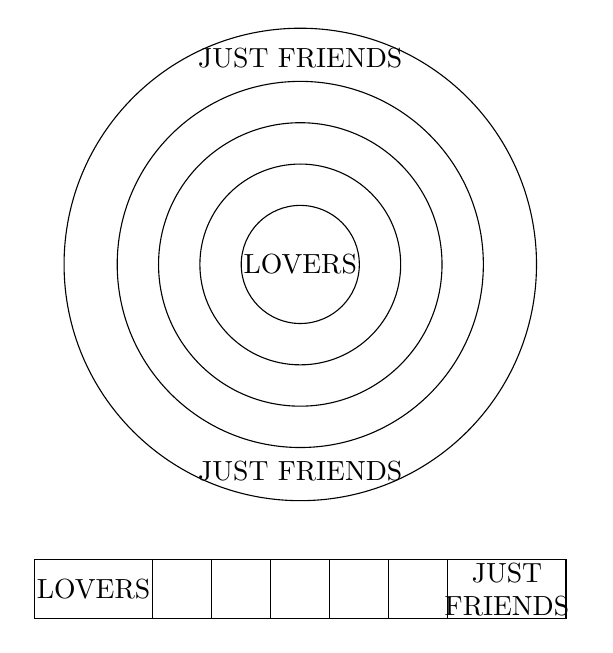
\begin{tikzpicture}[scale=0.75]
\begin{scope}
\draw circle (1) circle (1.7) circle (2.4) circle (3.1) circle (4.0)
  (0,0) node {LOVERS}
  (0,3.5) node {JUST FRIENDS}
  (0,-3.5) node {JUST FRIENDS};
\end{scope}
\begin{scope}[yshift=-5cm]
\draw
  (-2.5,0) rectangle +(-2,-1)
    +(-1,-0.5) node [anchor=center] {LOVERS}
  (2.5,0) rectangle +(2,-1)
    +(1,-0.5) node [text width=1.75cm,text centered] { JUST FRIENDS}
  \foreach \x in {-2.5,...,1.5} {
    (\x,0) rectangle ++(1,-1)
  }
;
\end{scope}
\end{tikzpicture}

\caption{Sample social combat map: Seduction}
\label{fig:social-combat-map-seduction}
\end{figure}

% \newpage


A seduction might be well modeled with a deep set of concentric circles --- say five or six --- with the objective of getting both characters in the bull's-eye (such as in \autoref{fig:social-combat-map-seduction}). Such an engagement could have multiple suitors and possibly require removing some or all from the map through Composure damage.

Suitors might be PCs or they might be NPCs or in some cases they might just be ``pawns'' --- if there is a concept you want to be relevant to the goal but that doesn't necessarily need to have free will in the fight, just give it a marker and no statistics. Players can move it around towards or away from goals (voters in an election or observers at a debate!) but it doesn't do anything on its own.

This could also be done with a simple linear track of, say, seven zones. Mark the first zone \LOVERS{} and the last zone \JUSTFRIENDS{}. Start the seducer on or near \LOVERS{} and the objective on or near \JUSTFRIENDS{}. Start other competitive suitors anywhere that seems fun or scary.

If the objective and anyone else are together on the \LOVERS{} zone, it has fallen for that suitor. If the objective and anyone else are together on the \JUSTFRIENDS{} zone, whoever has joined the objective there is removed from play.

% \newpage

\subsubsection{Debate}

\begin{figure}
\centering\footnotesize
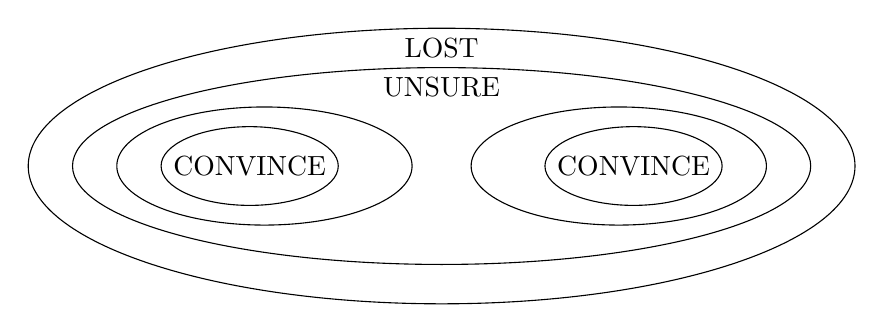
\begin{tikzpicture}[xscale=0.75,yscale=0.5]
\begin{scope}
\draw
  (-3,0) circle (2.5 and 1.5)
  (-3.25,0)   circle (1.5 and 1) node {CONVINCE}
  (0,0) ellipse (7 and 3.5) (0,3) node {LOST}
  (0,0) ellipse (6.25 and 2.5) (0,2) node {UNSURE}
  (3,0) circle (2.5 and 1.5)
  (3.25,0)   circle (1.5 and 1) node {CONVINCE}
%   (-3,0) node {CONVINCE}
%   (0,3.5) node {JUST FRIENDS}
%   (0,-3.5) node {JUST FRIENDS}
;
\end{scope}
% \begin{scope}[yshift=-5cm]
% \draw
%   (-2.5,0) rectangle +(-2,-1)
%     +(-1,-0.5) node [anchor=center] {LOVERS}
%   (2.5,0) rectangle +(2,-1)
%     +(1,-0.5) node [text width=1.75cm,text centered] { JUST FRIENDS}
%   \foreach \x in {-2.5,...,1.5} {
%     (\x,0) rectangle ++(1,-1)
%   }
% ;
% \end{scope}
\end{tikzpicture}

\caption{Sample social combat map: Debate}
\label{fig:social-combat-map-debate}
\end{figure}

% \newpage

A debate can be modeled with two sets of concentric circles representing opposing perspectives (see \autoref{fig:social-combat-map-debate}). The objective would be to move the opponent into your own central circle or moving the majority of audience members into your zone. Note that because of the steep drop-off in effectiveness at range, it will be necessary to move towards your opponent in order to engage him and pull him back to see your point (answering his specific arguments, showing sympathy and understanding).


\section{The Sequence}\label{sec:The Sequence}

Space combat is played in turns, each of which might represent fifteen to thirty minutes of in-game time --- this too has been largely abstracted. Each turn consists of several phases, and each phase will offer a test --- an opportunity to cross-compel, a roll, and an opportunity to tag and/or invoke \Aspects.

\subsection{Detection}
\label{sec:Detection}

% \makeatletter
% \newsavebox{\hbbox}%
% \begin{lrbox}{\hbbox}
% \begin{minipage}[c]{3.8cm}
% \sideboxtitle{Phases}
% The phases are:
% \begin{enumerate}
% \item Detection
% \item Position
% \item Electronic warfare
% \item Beam
% \item Torpedo
% \item Damage control
% \end{enumerate}
% \end{minipage}
% \end{lrbox}
% \begin{wraptable}{r}[\sidebarwidth]{0cm}\end{wraptable}
% \makeatother

% ~

\begin{wraptable}{r}[\sidebarwidth]{5cm}
\centering
% \begin{halfbox}{r}{5cm}{Phases}
\newsavebox{\hbbox}%
\begin{lrbox}{\hbbox}
\begin{minipage}[c]{4.5cm}
\sideboxtitle{Phases of space combat}
% The phases are:
\begin{enumerate}
\item Detection
\item Position
\item Electronic warfare
\item Beam
\item Torpedo
\item Damage control
\end{enumerate}
\end{minipage}
\end{lrbox}
\colorbox{sbbackground}{\usebox{\hbbox}}
% \caption{#5}
% \label{#6}
% \end{halfbox}
\end{wraptable}

Before a fight can start, everyone needs to find each other. Position is plotted on a linear scale from -4 to +4 on the map. As always, before any dice are rolled, the caller will ask for compels, at which time players can compel each other to fail to act. Failure to act in this case is represented by an automatic result of -4 (dice are not rolled and \Skills\ are not considered: your final result for your \Navigation\ check is -4).

A \Navigation\ check is rolled by each ship's navigation officer, and all rolls are ranked. Ties are resolved by raw \Navigation\ \Skill. The highest ranked Navigator will place two of the ships to be played on the map anywhere except the two most distant lines (-4 and 4). The next highest rank then places a single ship and this continues until all ships are placed. The lowest ranking Navigator places nothing. The ship which wins the detection round may also decide if there will be a positioning roll in the first turn (only). Once all the ships are placed, the winning ship in this phase decides whether to proceed to phase 1 or directly to phase 2. This allows a ship to attempt escape without engaging in combat immediately on being detected --- going to phase 1 --- or it allows it to use the tactical position from the detection phase for an optimized initial combat round --- going to phase 2.

In the event of a tie between two ships (as might happen when two standard T2 merchant ships meet, with default navigators), if neither ship is willing or able to invest fate points to gain victory, ships are placed randomly, based on a roll of the fate dice (it is only in this circumstance that a ship may begin at the 4 or -4 band).

\subsection{Position}\label{sec:Position} % \href{sec:id143}

As always, before any dice are rolled, the caller will ask for compels, at which time players can compel each other to fail to act. Failure to act in this case is represented by an automatic result of -4 (dice are not rolled and Skills are not considered: your final result for your positioning check is -4).

Spacecraft positions are plotted on a simple linear scale from -4 to +4. Ships begin as they were placed in the detection phase. At the beginning of each round of combat, pilots jockey for position. All pilots roll their ship's V-shift rating limited by their effective Pilot Skill (i.e. if one character is serving both as Navigator and Pilot, then the Pilot's effective Pilot Skill is reduced by one). Note also that this is not simply a modifier to the roll: since V-shift is limited by effective Pilot Skill, this penalty might affect performance for the first turn as well.

In addition, ships may apply burn: by running their drives over rating, they can exchange Heat for an advantage in maneuver, improving the V-shift roll. Any ship may declare that it is applying burn, state the value and add that value to their roll (not to the V-shift rating). They immediately take a hit to their Heat stress track equal to the value of their burn, marking that box and all unmarked boxes below it. If the highest box to be marked is already marked, mark the next higher open box. Before marking the damage to the Heat stress track, the pilot may reduce the detrimental effects through Consequences exactly as mitigating combat damage. The caller may allow negotiation of burn declarations at his preference, though generally a declared burn rating by a ship's player must stand.

Ships may choose not to use their drives in order to bleed heat. Each turn that the V-Shift is not engaged allows the highest filled box in the Heat track to be cleared immediately. This decision results in an automatic -4 final result for the positioning check, which might still be modified by Aspects, but no dice are rolled and no Skill is used. No burn declarations can be made once the caller declares the bidding closed and asks for dice on the table.

Only the highest roller may alter any ship's positions:
\begin{itemize}
\item He may move himself the difference between his roll and the lowest roll, or
\item He may move any ship with a lower roll up to the level of the
difference between them.
\end{itemize}

He may not, however, move any vessel more map bands than his own vessel's V-shift rating. Remember, moving a ship between the 3 and 4 bar (or the -3 and -4) costs 2 shifts, and moving a ship from the last bar off the map costs 3 shifts.

If the winning positioning roll is tied, the next highest roll is the winner. This presents some interesting tactical choices for fate point expenditure: sometimes it's advantageous to forfeit your awesome roll so that your ally, who rolled lower, can make use of his better V-shift, for example. You might then use an Aspect to force a tie so that you lose control.

If a ship exceeds the band at -4 or 4, they leave combat, whether forced off by others or maneuvered off by their own pilots. In this fashion a really excellent pilot in a hot ship can cut down the odds by positioning enemy vessels off the map until he faces only one opponent. Similarly, more than two ships chasing a single ship can usually keep the lone opponent on the map through positioning.

\subsection{Electronic Warfare}\label{sec:Electronic Warfare}
\vfil
As always, before any dice are rolled, the caller will ask for compels, at which time players can compel each other to fail to act. Failure to act in this case is represented by the ship being unable to declare a target.

Before any destructive weapons are used, each ship may conduct electronic warfare, pitting its communications officer against the enemy. If a communications officer has \stunt{Military-grade Communications}, she may pick a target and roll the ship's \skill{Electronic Warfare} (EW) rating, amplified by her effective \skill{Communications} Skill (if the communications officer has acted in any of the previous phases, there is a cumulative -1 penalty for each phase she has acted). The defender also makes a roll, of his ship's \skill{EW} rating, amplified by the communications officer's effective \skill{Communications} Skill. The rating may be zero, in which case there is there is no crewman staffing the position unless this is done by one of the PCs. Ships may have a Stunt (\stunt{Firewall}) that automatically provides a defense value of 2, and which may not be modified. Subtract the defender's modified roll from the attacker's.

As with any roll, these results can now be modified by tagging or invoking \Aspects\ and paying a fate point to get +2 or re-roll.

Positive values are treated as shifts against the defender, and
%
negative values are treated as shifts against the attacker.
%
Whoever has shifts against him will take a \Data\ stress track hit to the ship. Before damage is calculated, the player may apply \Consequences\ to reduce the number of shifts: a mild Consequence reduces the shifts by one, a moderate Consequence reduces the shifts by two, and a severe Consequence reduces the shifts by four. Recall that no entity can have more than three Consequences of any kind and never more than one of each type.

% \newpage

Once the final number of shifts are determined, the corresponding box on the \Data\ stress track is marked and all open boxes below it are also marked. If the highest box to be marked has already been marked, mark the next highest open box.

Note that only one roll is made for each ship, so in some cases with more than two ships in play, a single roll may defend against multiple attacking rolls as well as conceivably acting as the attacking roll on a declared target. Note also that a good defense against hacking can inflict damage on the attacking \Data\ stress track, even if the defending communications officer does not have Military-grade \skill{Communications}.

The Electronic Warfare (EW) defense roll is persistent through this phase, but the total may be added to over the course of the phase through the spending of fate points. An outnumbered ship may still mount a reasonable defense.

% \newpage

\subsection{Beam Weapons}\label{sec:Beam Weapons} % \href{sec:id145}

Beam weapons subsume all relatively short range unguided weaponry, so they may be described as lasers of various wavelengths, artillery, rockets, railguns, electromagnetically propelled storms of small projectiles, particle beams, or anything else that suits the setting developed at the table. Beams are used both offensively, to directly damage targets at shorter ranges, and defensively, to defend against torpedoes (see Torpedo phase for details).

As always, before any dice are rolled, the caller will ask for compels, at which time players can compel each other to fail to act. Failure to act in this case is represented by a failure to declare a target in whatever phase the player ship was compelled.

A ship with a Beam Skill can attack at any value from 1 up to the full Beam rating. When Beams are fired offensively the attacker must declare what Beam rating he will apply. Note the Beam value used, as it will be relevant in the Torpedo phase.

All combat rolls are made at the Beam rating amplified by the gunner's Gunnery Skill (that is, the Beam rating is used and increased by one if the Gunnery Skill is higher). If the gunnery officer has acted in any of the previous phases, there is a cumulative -1 penalty to the effective Skill level for each phase he has acted. 

Beams firing at three or more bands range subtract 2 from the roll. Attacks are resolved as they are declared, again leveraging social pressure to determine who goes first: the caller closes the call for targets by announcing a final call, and counting slowly to three (if necessary --- if your caller is fair and fun, he'll leave plenty of time), after which no further targets can be announced.

There is no skill to defend against Beams. A roll with no modification is made to oppose all incoming Beam attacks. Ship's may have a Stunt (Vector Randomizer) that changes the base from 0 to 2.
Defensive rolls are made once for each defensive system but stay on the table --- that defensive roll you made against Beams stands throughout the Beam Weapons phase, complete with any modifications from invoking Aspects, using spin, etc. Defensive rolls are persistent through the phase, so it can be handy to note them on the ship card or use a coloured 12- or 20-sided die set to the result. Sometimes we write them on the map. Offensive Beam rolls are distinct from defensive Beam rolls (from the Torpedo phase) and should be recorded separately.

% \newpage

Subtract the defender's final sum from the attacker's to find the number of shifts, and thus the amount of stress on the defender's \Frame\ track. The defender may reduce these by applying one or more Consequences:
\begin{itemize}
\item reduce the shifts by one by applying a mild Consequence
\item reduce the shifts by two by applying a moderate Consequence
\item reduce the shifts by four by applying a severe Consequence.
\end{itemize}

Recall that no entity may have more than three Consequences and never more than one of each kind.

% \newpage

\subsection{Torpedoes}\label{sec:Torpedoes} % \href{sec:id146}

As always, before any dice are rolled, the caller will ask for compels, at which time players can compel each other to fail to act. Failure to act in this case is represented by a failure to declare a target in whatever phase the player ship was compelled.

Torpedoes attack at the spacecraft's Torpedo Skill rating, amplified by the gunner's effective Gunnery Skill (that is, the Torpedo rating is used and increased by one if the effective Gunnery rating is higher). If the gunnery officer has acted in any of the previous phases (including the Beam phase), there is a cumulative -1 penalty for each previously active phase.

Torpedoes firing at one or zero bands range subtract 2 from the roll. Attacks are resolved as they are declared, again leveraging social pressure to build an initiative order as in the Beam phase. The caller closes the call for targets by announcing a final call, and counting slowly to three, after which no further targets can be announced.

A Beam roll is made to oppose all incoming Torpedoes. To do this, the beam position must be staffed. If Beams were fired in the Beam Weapons phase, then the roll may be made as usual, amplified by gunner's effective Gunnery Skill. If Beams were not fired, then there must be a trained crew member available to man the beams in this phase: normal penalties and bonuses apply, but since each crew member may only act once per phase, a ship with a single gunner (as might happen with a skeleton crew) may have to choose between offensive Torpedo fire and defensive Beam fire. Beams so used may also have been fired offensively, and defensive fire may cause damage to the Heat stress track. Ships with no Beam rating or those unwilling to fire Beams defensively, roll with a base of 0 unless they have a Stunt (Point Defense) that changes the base from 0 to 2.

Defensive rolls are made once for each defensive system but stay on the table --- that  defensive roll you made with the Beams stands throughout the Torpedo Phase, complete with any modifications from Aspect invocation, spin, or other sources. As these rolls are persistent through the phase, it can be handy to note them on the ship card or use a coloured 12- or 20-sided die set to the result. Sometimes we write them on the map. Though persistent, defensive rolls are distinct from offensive rolls and should be recorded separately.

% \newpage

When Beams are fired defensively the attacker must declare what Beam rating he will apply. He may apply any value from 0 to the full Beam rating. Note the Beam value used. If the sum of the offensive Beam used in the Beam phase plus the defensive Beam used in the Torpedo phase is greater than the total Beam rating, then the ship takes a hit on the Heat stress track equal to the difference and marks all boxes below as well.

Subtract the final defender's sum from the attacker's to find the number of shifts, and thus the amount of stress on the defender's \Frame\ track. The defender may reduce these by applying one or more Consequences:
\begin{itemize}
\item reduce the shifts by one by applying a mild Consequence
\item reduce the shifts by two by applying a moderate Consequence
\item reduce the shifts by four by applying a severe Consequence.
\end{itemize}

Recall that no entity may have more than three Consequences, nor more than one of each kind.

% \newpage

\subsection{Damage Control}
\label{sec:Damage Control}

Damage control checks may now be made on Frame stress tracks (using one crew member's effective \skill{Engineering} Skill) or Data stress tracks (using one crew member's effective \skill{Computer} Skill). Since each crew may only staff one position per phase, the same individual may not be responsible for both rolls. If the engineer or computer officer has acted in any of the previous phases, there is a cumulative -1 penalty for each previously active phase. The target number for success is the highest box marked on the relevant track. The number of successes indicate the track box that can be erased. Erase it and all unmarked boxes below it.

The Heat stress track cannot be repaired during combat, except by shutting off engines, as described in the positioning phase.


\section{Damage}\label{sec:social-combat-damage}

Stress box hits are not real damage, but they can lead to Consequences. All stress box hits are removed after a few days of relaxing stress-free downtime. As with personal combat, the table should rule when enough time has passed or whether the downtime was sufficiently relaxing. Generally speaking it should be trivial.

\subsection{Recovering Consequences}\label{sec:social-combat-recovering-consequences}

A mild Consequence can be self-medicated with a bottle and some time alone once the scene is over. No roll is required and it is cleared as soon as the social combat scene is over.

A moderate Consequence remains until the end of the session in which it was incurred.

A severe Consequence must be carried through one complete session in which the associated stress track is never marked. If it is incurred during session one, it is gone no sooner than the end of session two, and if the associated stress track takes hit in a fight during that session, you'll need to hold the Consequence through yet another one.


\section{Special Rules}\label{sec:personal-combat-special-rules}

\subsection{First Blood}\label{sec:personal-combat-first-blood}

Getting shot is scary. Even when you are a professional. When a player marks a \Health{} stress track hit and has not yet marked any \Health{} or \Composure{} boxes, the \Composure{} stress track is also marked at the same value (and all boxes below, as always). After this initial combat shock all attacks are against \Health{} or \Composure{} but not both.

Note that Consequences reduce shifts \emph{before} they are marked as damage, so they do not have to be applied separately for each track here.  This means that when first hit, a player must decide whether to take a Consequence that will have a doubled effect (but making the character more vulnerable in subsequent rounds) or decide to tough it out in hopes of finishing the fight quickly.

\subsection{Out of Ammo}\label{sec:out-of-ammo}

Who wants to count bullets? Not us. It's way more fun to have an Aspect, and let your opponents decide when you run out of bullets. Anyone using a slug thrower automatically gets the Aspect \aspect{Out of ammo} to be compelled liberally, but which cannot be free-tagged.

Anyone who has used a slug thrower to make an Area of Effect attack (using the \stunt{Full Auto} stunt) gets the Aspect \aspect{Out of ammo} to be compelled liberally, and it can be free-tagged each time the weapon is used for an Area of Effect attack.

\subsection{Military-Grade and Civilian}
\label{sec:military-grade-and-civilian}

The use of any weapon or armour that does not have the \stunt{Civilian} Stunt requires a Military-grade Skill. It may be the case that it is sufficient at some tables to deny access and not explain, but it might be more satisfying to have a mechanism. A character without the appropriate Military-grade stunt can use the military equipment (at her Skill level), but only by paying a fate point for each roll. Thus the player can have her character use the superior but unfamiliar equipment, but with an attendant loss in fate points.

\subsection{Hostile Environments}\label{sec:hostile-environments}

Sometimes a fight will take place in an environment where the integrity of armour is important not only to absorb combat damage but also to resist environmental effects. These environments might include low pressure, high pressure, or toxic atmospheres. In these cases a loss of suit integrity has serious ramifications. A hostile environment suit has lost integrity when the wearer takes any \Health{} track Consequence.

\iflandscape{}{\vfil}
\subsection{Zero Gravity}\label{sec:zero-gravity}

When fighting in zero or low gravity the scene has the Aspect \aspect{Zero gravity} or \aspect{Low gravity}. This can be tagged as usual by participants.

Some weapons are recoilless, and are designed for low gravity. These have the \stunt{Low Recoil} Stunt. All attacks using weapons without the \stunt{Low Recoil} Stunt use the \skill{MicroG} Skill instead of their preferred Skill (\skill{Brawling}, \skill{Close Combat}, \skill{Slug Thrower}). The \skill{MicroG} Skill does not confer knowledge of the maintenance and repair of any weapons: for that, checks need to be made against the relevant weapons Skill.

\skill{MicroG} rolls may also be called for to perform movement or other activity in zero or low gravity.

The referee may determine additional penalties that apply in MicroG environments: without a handhold, it simply may not be possible to throw a grenade effectively.

In some contexts the shifting of gravity can lead to interesting play environments. This might lead to a permanent penalty on all action in the scene. For example:
\begin{description}
\item [Sloping gravity]
the ship is rotating under thrust. All actions are done as if in gravity (i.e. without the \skill{MicroG} Skill) and are at -2
\item [Stuttering microgravity]
a drive keeps kicking in and out. All actions are as in micro-G, but at -1
\item [Low gravity]
all actions are at -2, using the better of \skill{MicroG} or the relevant combat Skill.
\end{description}

These environmental effects may be determined by the referee as the map is designed, or they may be a consequence of player actions.


\section[Wargaming]{Wargaming}
\label{sec:personal-combat-wargaming}

Sometimes it's fun just to make one-off characters and have them shoot at each other. To play independently as a tactical war game, you need three things: a map, a story, and characters.

\subsection{The Map}
\label{sec:personal-combat-wargaming-map}

Someone is chosen as caller. Either the caller or the table draws a map. Is it a shoot out in an airport? A race to secure a bunker at the top of a hill? A boarding action in a submarine or a spaceship? Whatever the case, you need a map to play on.

You can start with a blank piece of paper, and take turns drawing features, until it looks good enough. Feel free to write words on the map too – these can become Aspects and help clarify what's what.

Once that is done, divide the map into zones. You don't want too many, but enough to allow opportunities for getting outside of range, and to allow movement. When drawing zones, it is often helpful to go from corner to corner: that means it is always clear when a character enters an area (from a door, or otherwise along a side) what zone he is in.

\subsection{The Story}
\label{sec:personal-combat-wargaming-story}

The process of drawing a map has already begun to determine what the story is: is this a fight to the death? Are there teams? Is most of the table maneuvering against a small cadre controlled by the caller (or by someone else)? Is there a difference in tech level between two sides? Whatever the case, articulating the story that is being told might mean that you go back and change the map slightly, add an Aspect to a zone or two, or whatever.

Most important is that the story articulates victory conditions, which need not be the same for all players. Is this a fight to the death? An attempt to capture someone alive? Someone working to escape detection and get out of a building, or sabotage a spacecraft's drives? Whatever the case, the victory condition might be defined in terms of time: get off the ship in eight turns; spend two turns alone in the engine room setting explosives.

\subsection{Characters in Wargaming}
\label{sec:characters-in-wargaming}

\iflandscape
{\begin{wraptable}[14]{r}[0.9\sidebarwidth]{5cm}}
{\begin{wraptable}[14]{r}[0.9\sidebarwidth]{5.5cm}}
% \begin{table}[ht]
\centering
\begin{tabular}{ll}\toprule
Skill & type \\
\midrule
Agility		\\
Alertness	\\
Brawling	& combat \\
Close Combat	& combat \\
Energy Weapons	& combat \\
EVA		\\
MicroG		\\
Resolve		& track \\
Slug Throwers	& combat \\
Stamina		& track \\
Stealth		\\
Tactics		\\
\bottomrule
\end{tabular}
\caption{Useful skills for personal combat wargaming}
\label{tab:personal-wargaming-skills}
% \end{table}
\end{wraptable}


Once the map and the story are determined, everyone should spend five minutes (no more) making one or two characters to push around the map.

\subsubsection{Skills}

Given the limited focus of this tactical game, 3-cap characters should be sufficient: pick one Skill at level 3, two at level 2, and three at level 1. Everything else is considered untrained. While any Skill might be taken, \autoref{tab:personal-wargaming-skills} presents Skills particularly relevant to this mini-game.

\subsubsection{Stress Tracks}

Characters should only concern themselves with the \Health{} and \Composure{} stress tracks. Each is three boxes long. If the character has \skill{Resolve} at level 1 or 2, the \Composure{} track has four boxes; if he has \skill{Resolve} 3, the \Composure{} track has five boxes. If the character has \skill{Stamina} at level 1 or 2, the \Health{} track has four boxes; if he has \skill{Stamina} 3, the \Health{} track has five boxes.

\subsubsection{Stunts}

Every character selects a Stunt. Making something Military-grade or altering how a stress track works are both obvious choices. (For some stories, it may be desirable to allow two Stunts per character; that's fine, as long as it's the same across the board).

\subsubsection{Aspects}

Each character should have three Aspects, revealed to all at the table. Each character also begins with three fate points.

Making a note card for each character, placed in front of the player with all the relevant information and a small pile of fate points stacked on top keeps all the information clear at all times. This is obviously scaled back from the RPG, and introduces a slightly different calculus for what constitutes a success. With reduced characters, teamwork, particularly in laying down maneuvers to be free-tagged, is rewarded.

\section{Equipment}
\label{sec:Equipment}

Characters should be considered to start with whatever equipment is relevant to their Skills and any trivial equipment should be present if needed unless lacking the item advances the plot. The only equipment that is guaranteed to be with the character when they need it is equipment that is represented by a ``Have a thing'' Stunt.

The referee cannot take away equipment specified as a Stunt from a player's character unless the player agrees and the Stunt is changed. This does not imply that an owned spacecraft (through a Stunt) cannot be Taken Out in combat, but rather that Taken Out cannot mean total loss of the craft with no chance of repair or replacement, unless the owning player agrees.

Rather than itemizing in a list, starting gear is assumed based on the Skills players select for their characters; quality of gear might also be affected by the Skill level: a character with EVA 1 might have an old T1 suit worn by her father; a character with EVA 4 might have a sleek T3 suit, custom fitted.

\subsection{Automatic Skill Gear}
\label{sec:automatic-skill-gear}

% \begin{tablebox}{Automatic Skill Gear}
\begin{table*}[htb]
\centering
\begin{tabular}{*2{lp{0.65\columnwidth}}}
\toprule
Skill		& Gear &
Skill		& Gear \\
\midrule
Agility		& access to a gym. &
Gunnery		& certification. \\
Aircraft	& certification, silk scarf. &
MicroG		& velcro shoes. \\
Arts		& toolkit, or database of relevant information. &
Navigation	& certification, computer with database of star charts for the cluster. \\
Brawling	& gold teeth. &
Pilot		& a license to fly in system (certification). \\
Brokerage	& certification, contacts. &
Profession	& player choice based on chosen profession. \\
Bureaucracy	& a personal organizer and communicator. &
Resolve		& sunglasses. \\
Close Combat	& one appropriate weapon. &
Science		& database of relevant information. \\
Communications	& hand computer. &
Slug Throwers	& a slug thrower. \\
Computer	& hand computer. &
Stamina		& running shoes. \\
Energy Weapons	& an energy weapon. &
Survival	& emergency kit, rations. \\
Engineering	& an iron ring (certification), toolkit, access to a machine shop. &
Vehicle		& certification, fuzzy dice.\\
EVA		& a pressure suit. \\
\bottomrule
\end{tabular}
\caption{Automatic Skill Gear}
\label{tab:automatic-skill-gear}
\end{table*}
% \end{tablebox}


Some Skills imply access to some kinds of equipment. Below are a list of associations that one can afford to take for granted, though, unless the equipment is represented by a ``Have a thing'' Stunt, it's not guaranteed to always be with the character --- it can be lost or destroyed. This list can be extended, according to the decision of the table: the standard is \emph{whatever's reasonable}.

Nothing guarantees the continued presence of the equipment, unless there is also an Stunt to cover it.

Many people will want the highest technology gear for their characters, and it is worth keeping track of the technology rating of anything purchased, if only because that can possibly serve as an Aspect at moments of crisis. Nevertheless, things do not stay at the same quality once they are invented, and a T3 hand computer will be far superior to a T0 one.

Creativity can be rewarded, especially when the benefits come at the level of role-playing, rather than at the level of the specific combat sub-games. A highly advanced knife might not do any more damage, but perhaps is made of a memory plastic --- when inactive, it is a simple cylinder of plastic but becomes activated by smacking it against a hard surface, and the cylinder deforms to become a hard, sharp, combat blade.

Similarly, an energy weapon might have a biometric check associated with it, allowing only the owning player to use it (this would be similar to making the weapon integral). Something like this might be hard to find, and it may be illegal, but it does not require a special Skill or Stunt to use.



\chapter{Space Combat}\label{sec:space-combat} % \href{sec:id136}

\begin{sidebox}{Original Material}

The \href{http://www.vsca.ca/Diaspora/Space%20combat%20demo.pdf}{original chapter about Space Combat}
is available from the Diaspora Website:
\begin{center}\verb#http://www.vsca.ca/Diaspora/Space%20combat%20demo.pdf#\end{center}
\end{sidebox}


Spacecraft are large, relatively fragile things pursuing their goals at high velocity in the dead of space. They are constrained by their available reaction mass, the mass  allocated for trade cargo, and their ability to dissipate heat. When they test each other to destruction using the assorted weapons of space combat --- beams, torpedoes, and electronic warfare --- they are chiefly pursuing goals of domination or escape. This system emphasizes these goals. The stories we want to tell include:

\begin{itemize}
\item an inferior ship escaping from the authorities
\item a hostile vessel capturing cargo
\item a threat so powerful the only real option is to surrender
\item a convoy of merchants and escorts safely defending itself from marauders
\end{itemize}

Space combat occurs on a simple map that emphasizes pursuit in order to provide a simple and fast system.

Combat occurs in phases. First is the detection phase which establishes the initial positions. Then the positioning, electronic warfare, beams, torpedoes, and damage control phases are repeated in order until everyone is happy, dead, or escaped. Order of action is controlled by social pressure: a player is designated caller for the fight and that person controls the transition from phase to phase (see sidebar on ``Social Initiative''). If a player wants to act in a particular phase, he announces his action. The advantage of going first goes to the one that speaks first. The advantage of going last goes to the person who speaks last. When the caller calls for a change of phase, it is possible that some players failed to act in time.

\section{The Crew}
\label{sec:the-crew}

Diaspora assumes that spacecraft have a fully functional crew aboard, who draw a salary and are able to man their stations competently.  There is no need to flesh them out unless there are role-playing reasons to do so, and player characters can work beside an undifferentiated crew happily.

Except as noted below, all combat crew positions on a ship are assumed to be staffed by someone with a \Skill\ level of 2.  PCs serving aboard such ships may use their individual \Skill\ levels, but if they choose not to (e.g. if they ride as passengers), there is always someone who can do the job.

A ship's \Trade\ value is not used in combat, and therefore there is no default broker aboard to assist with maintenance rolls.

The exception to this is a spacecraft that has the \stunt{Skeleton Crew} \Stunt, in which case all the jobs in combat must be taken by a known individual (either a player character or an NPC who has been developed) who is trained in the relevant \Skill. In particular, \skill{Communications} and \skill{Gunnery} stations, if they have a positive value, may not be operated by an untrained individual.

For each crew position, there is only ever one person doing a given job at a given time. One Navigator rolls in the detection phase, and only one Computer expert rolls to repair the \Data\ track.

A PC may occupy more than one position on the ship, but it becomes challenging during combat. Each \Skill\ associated with a combat phase normally requires a single crew member to staff it.

\rulebox[Staffing more than one post earns a -1 cu\-mu\-la\-tive penalty to 
effective Skill level]{Staffing more than one crew position during combat earns a -1
cumulative penalty to the effective Skill level.}
For example, a gunner may fire beams offensively and defensively without penalty, but would receive a penalty on the torpedo roll if he has fired beams.

\rulebox[Each crew member may act once per phase]{Each crew member may only act once per phase in combat.}
For example, a single gunner may not fire beams defensively and launch torpedoes in the same phase.


\section{Spacecraft}
\label{sec:spacecraft}

Spacecraft are the unit of scale in this mini-game, and not player characters. They have their own \Skills\ (\Vshift, \skill{Electronic Warfare}, \skill{Beams}, and \skill{Torpedoes}), \Stunts, \Aspects\ and stress tracks (\Frame, \Data\ and \Heat). The mini-game will involve rolling those \Skills to achieve results and marking damage against those stress tracks.

Spacecraft can mitigate stress hits with three \Consequences, just as characters do. You will find a list of ships at the end of the chapter, and later a method for creating your own.

Spacecraft not designated as \stunt{Civilian} can only be flown by characters with the \stunt{Military-grade Pilot} Stunt. Further, offensive use of the \skill{EW} ship Skill can only be done by characters with the \stunt{Military-grade EW} Stunt. Aspects listed are meant as suggestions: every ship has its own quirks and personality.


\section{The Map}\label{sec:social-combat-map}
% \vfil

Social combat takes place on a zone map much as it does with personal combat. Instead of representing some physical geography, the map represents the social space of the encounter. Because of the kinds of options available to characters involved in social combat, certain kinds of map shapes have certain kinds of effects on behaviour and can be used to represent specific issues.

In general, concentric circles imply intimacy. Zone shapes with many borders, and therefore many avenues of escape and access, better represent socially open places like chatting about the weather at a party. Intimate zones are often objectives, such as when you want to get someone to reveal valuable information, and so you want to maneuver them into intimate, trusting conversation.

% \newpage

To begin with, moving between zones has no additional cost --- there is no initial use of ``borders'' as there is in personal combat. Characters in the same zone can be said to be engaging each other socially: they are conversing about interesting, relevant things that they care about. Conversely, the further apart characters are on the map, the more social distance is in their conversation. Range has a deep impact on the effectiveness of characters' interactions and so one must usually close the range before one can do anything useful, such as move the conversation to a more intimate space.

% \newpage

Zones represent in the first instance a degree of intimacy in the social context. This will sometimes correspond to a spatial dimension too, but more often it represents something much more nebulous. For instance, a separate zone might correspond to a small balcony where a conversation might occur. It is often a good idea for the table to design the map of the social combat as a group.

Optionally, once the map is created, each player may choose to place one free-taggable \Aspect{} on a single zone, or a pass value of 2 on a single border, to reflect the personal contours of the social situation.

% badbox here
% \newpage

\subsection{Time}\label{sec:Time}

For each zone on the map, create one time box to represent available time to resolve. If you need to know exactly how long something took, the table should determine the maximum amount of time something is allowed (even the best party will disperse by morning). If a victory condition is achieved before the time boxes run out, the maximum time can be downgraded a number of shifts on the Time Track (Dealing With Time, Chapter 2) equal to the number of unchecked boxes. Often, table consensus will determine a very similar result in any case.

% \newpage

\subsection{The Actors}\label{sec:The Actors}

One of the biggest conceptual hurdles in adopting this system for resolving social interactions is recognizing that not every person in a scene needs to be represented on the map. Part of this is embodied within the zones themselves, as \Aspects{} on the zones can represent the other people involved.

This can in fact be made even more abstract, when you want to make a situation tactical that has become mired or unproductive in regular role-play. By making some of the actors on the map ideas instead of explicit people, you can conduct a scientific investigation or any other information-revealing multi-step endeavour. Make the opposition the Fact and, maybe, an Attractive Falsehood and you can do science. Add in people with conflicting goals (a young whipper-snapper who wants to be primary author on the publication of your discovery!) and the abstract can engage the concrete in both directions.

% \newpage

\subsection{Victory}\label{sec:Victory}

Victory conditions should relate to map position. Usually the objective will be to get a certain person or persons into a specific zone before the timer runs out. This can be more complex, however, to achieve different goals: if you want to model persuading a crowd, you could score participants by how many crowd members are in their target zone when the timer runs out. Feel free to push the system around and find other victory conditions.

\newpage

\subsection{Sample Maps}\label{sec:Sample Maps}

% \newpage

\subsubsection{Party}

A party has a lot of accessible conversation space --- everyone is there to chit-chat after all --- and probably at least one intimate space. It is well represented by a central shape with several attached shapes. Inside one attached space, add a couple of concentric circles for intimacy. An objective in the party might be to hook up with a powerful businessman and get him to brag about his company's secret operation on the dark side of the moon: you win if you can get him, yourself, and the science officer into the center of the intimate zone before the timer runs out.

The party map doesn't need to be complicated --- the simpler it is the faster things will go. The important thing is to make it take a few steps to get to the target zone and be complex enough to imply story with every move. The map above is about the minimum complexity you would want from a social combat map. It might be close to the maximum also!

% \newpage

\subsubsection{Seduction}

\begin{figure}
\centering\footnotesize
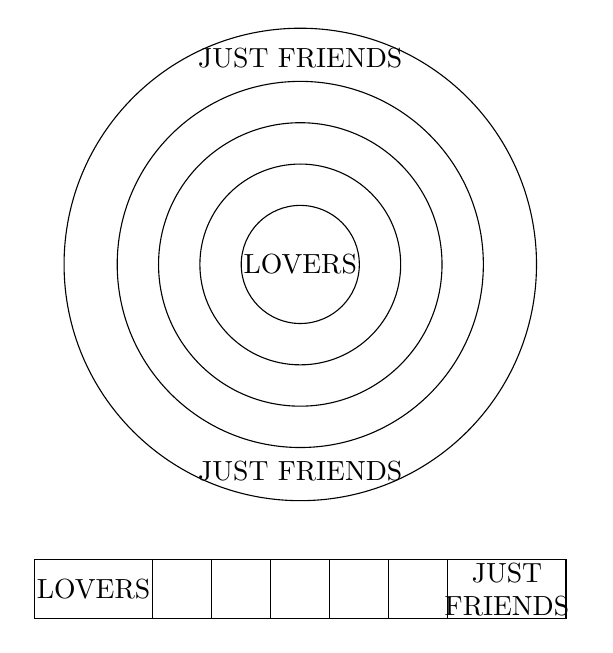
\begin{tikzpicture}[scale=0.75]
\begin{scope}
\draw circle (1) circle (1.7) circle (2.4) circle (3.1) circle (4.0)
  (0,0) node {LOVERS}
  (0,3.5) node {JUST FRIENDS}
  (0,-3.5) node {JUST FRIENDS};
\end{scope}
\begin{scope}[yshift=-5cm]
\draw
  (-2.5,0) rectangle +(-2,-1)
    +(-1,-0.5) node [anchor=center] {LOVERS}
  (2.5,0) rectangle +(2,-1)
    +(1,-0.5) node [text width=1.75cm,text centered] { JUST FRIENDS}
  \foreach \x in {-2.5,...,1.5} {
    (\x,0) rectangle ++(1,-1)
  }
;
\end{scope}
\end{tikzpicture}

\caption{Sample social combat map: Seduction}
\label{fig:social-combat-map-seduction}
\end{figure}

% \newpage


A seduction might be well modeled with a deep set of concentric circles --- say five or six --- with the objective of getting both characters in the bull's-eye (such as in \autoref{fig:social-combat-map-seduction}). Such an engagement could have multiple suitors and possibly require removing some or all from the map through Composure damage.

Suitors might be PCs or they might be NPCs or in some cases they might just be ``pawns'' --- if there is a concept you want to be relevant to the goal but that doesn't necessarily need to have free will in the fight, just give it a marker and no statistics. Players can move it around towards or away from goals (voters in an election or observers at a debate!) but it doesn't do anything on its own.

This could also be done with a simple linear track of, say, seven zones. Mark the first zone \LOVERS{} and the last zone \JUSTFRIENDS{}. Start the seducer on or near \LOVERS{} and the objective on or near \JUSTFRIENDS{}. Start other competitive suitors anywhere that seems fun or scary.

If the objective and anyone else are together on the \LOVERS{} zone, it has fallen for that suitor. If the objective and anyone else are together on the \JUSTFRIENDS{} zone, whoever has joined the objective there is removed from play.

% \newpage

\subsubsection{Debate}

\begin{figure}
\centering\footnotesize
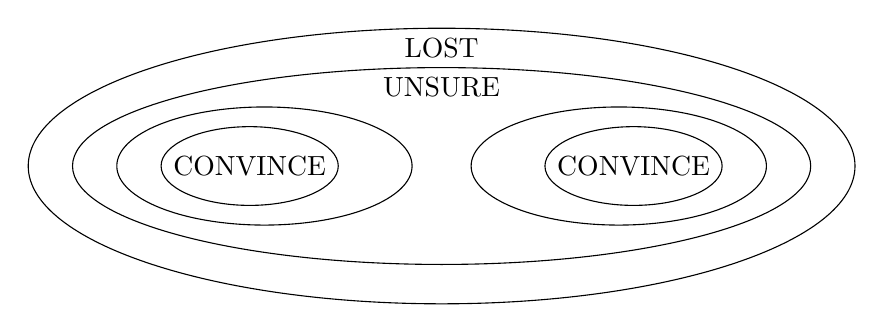
\begin{tikzpicture}[xscale=0.75,yscale=0.5]
\begin{scope}
\draw
  (-3,0) circle (2.5 and 1.5)
  (-3.25,0)   circle (1.5 and 1) node {CONVINCE}
  (0,0) ellipse (7 and 3.5) (0,3) node {LOST}
  (0,0) ellipse (6.25 and 2.5) (0,2) node {UNSURE}
  (3,0) circle (2.5 and 1.5)
  (3.25,0)   circle (1.5 and 1) node {CONVINCE}
%   (-3,0) node {CONVINCE}
%   (0,3.5) node {JUST FRIENDS}
%   (0,-3.5) node {JUST FRIENDS}
;
\end{scope}
% \begin{scope}[yshift=-5cm]
% \draw
%   (-2.5,0) rectangle +(-2,-1)
%     +(-1,-0.5) node [anchor=center] {LOVERS}
%   (2.5,0) rectangle +(2,-1)
%     +(1,-0.5) node [text width=1.75cm,text centered] { JUST FRIENDS}
%   \foreach \x in {-2.5,...,1.5} {
%     (\x,0) rectangle ++(1,-1)
%   }
% ;
% \end{scope}
\end{tikzpicture}

\caption{Sample social combat map: Debate}
\label{fig:social-combat-map-debate}
\end{figure}

% \newpage

A debate can be modeled with two sets of concentric circles representing opposing perspectives (see \autoref{fig:social-combat-map-debate}). The objective would be to move the opponent into your own central circle or moving the majority of audience members into your zone. Note that because of the steep drop-off in effectiveness at range, it will be necessary to move towards your opponent in order to engage him and pull him back to see your point (answering his specific arguments, showing sympathy and understanding).


% \section{Social Initiative}
\vfil\begin{sidebox}{Social Initiative}

\label{sec:Social Initiative}

The space combat mini-game operates using a form of social initiative. While often it is possible for the caller to start with one player who wants to act first and to proceed simply around the table, the stalemate-inducing anxieties of the uncertain commitment of resources over time can be fun to play with --- it creates the eerie feel of submarine combat, reducing the information available as decisions get made. For each of phases 1-4, the decision to act first resides with the player who states that they act first, with the caller determining priority if more than one person speaks at a time (or the table if the caller is controlling one of the affected ships).

% \rulebox{Resources, once com\-mit\-ted, can only be in\-creased.}

Going first entails a commitment of resources, and responses to the initial action can be proportionate, using the information of how much the first player has committed.
Resources, once committed, can only be increased.
They are never decreased.

As each phase ticks by, players may hold back attacking to wait until they see if they are being attacked and by how many, or they may strike hard and fast, filling their Heat track and hoping for a quick kill (or escape!).
\end{sidebox}

\section{The Sequence}\label{sec:The Sequence}

Space combat is played in turns, each of which might represent fifteen to thirty minutes of in-game time --- this too has been largely abstracted. Each turn consists of several phases, and each phase will offer a test --- an opportunity to cross-compel, a roll, and an opportunity to tag and/or invoke \Aspects.

\subsection{Detection}
\label{sec:Detection}

% \makeatletter
% \newsavebox{\hbbox}%
% \begin{lrbox}{\hbbox}
% \begin{minipage}[c]{3.8cm}
% \sideboxtitle{Phases}
% The phases are:
% \begin{enumerate}
% \item Detection
% \item Position
% \item Electronic warfare
% \item Beam
% \item Torpedo
% \item Damage control
% \end{enumerate}
% \end{minipage}
% \end{lrbox}
% \begin{wraptable}{r}[\sidebarwidth]{0cm}\end{wraptable}
% \makeatother

% ~

\begin{wraptable}{r}[\sidebarwidth]{5cm}
\centering
% \begin{halfbox}{r}{5cm}{Phases}
\newsavebox{\hbbox}%
\begin{lrbox}{\hbbox}
\begin{minipage}[c]{4.5cm}
\sideboxtitle{Phases of space combat}
% The phases are:
\begin{enumerate}
\item Detection
\item Position
\item Electronic warfare
\item Beam
\item Torpedo
\item Damage control
\end{enumerate}
\end{minipage}
\end{lrbox}
\colorbox{sbbackground}{\usebox{\hbbox}}
% \caption{#5}
% \label{#6}
% \end{halfbox}
\end{wraptable}

Before a fight can start, everyone needs to find each other. Position is plotted on a linear scale from -4 to +4 on the map. As always, before any dice are rolled, the caller will ask for compels, at which time players can compel each other to fail to act. Failure to act in this case is represented by an automatic result of -4 (dice are not rolled and \Skills\ are not considered: your final result for your \Navigation\ check is -4).

A \Navigation\ check is rolled by each ship's navigation officer, and all rolls are ranked. Ties are resolved by raw \Navigation\ \Skill. The highest ranked Navigator will place two of the ships to be played on the map anywhere except the two most distant lines (-4 and 4). The next highest rank then places a single ship and this continues until all ships are placed. The lowest ranking Navigator places nothing. The ship which wins the detection round may also decide if there will be a positioning roll in the first turn (only). Once all the ships are placed, the winning ship in this phase decides whether to proceed to phase 1 or directly to phase 2. This allows a ship to attempt escape without engaging in combat immediately on being detected --- going to phase 1 --- or it allows it to use the tactical position from the detection phase for an optimized initial combat round --- going to phase 2.

In the event of a tie between two ships (as might happen when two standard T2 merchant ships meet, with default navigators), if neither ship is willing or able to invest fate points to gain victory, ships are placed randomly, based on a roll of the fate dice (it is only in this circumstance that a ship may begin at the 4 or -4 band).

\subsection{Position}\label{sec:Position} % \href{sec:id143}

As always, before any dice are rolled, the caller will ask for compels, at which time players can compel each other to fail to act. Failure to act in this case is represented by an automatic result of -4 (dice are not rolled and Skills are not considered: your final result for your positioning check is -4).

Spacecraft positions are plotted on a simple linear scale from -4 to +4. Ships begin as they were placed in the detection phase. At the beginning of each round of combat, pilots jockey for position. All pilots roll their ship's V-shift rating limited by their effective Pilot Skill (i.e. if one character is serving both as Navigator and Pilot, then the Pilot's effective Pilot Skill is reduced by one). Note also that this is not simply a modifier to the roll: since V-shift is limited by effective Pilot Skill, this penalty might affect performance for the first turn as well.

In addition, ships may apply burn: by running their drives over rating, they can exchange Heat for an advantage in maneuver, improving the V-shift roll. Any ship may declare that it is applying burn, state the value and add that value to their roll (not to the V-shift rating). They immediately take a hit to their Heat stress track equal to the value of their burn, marking that box and all unmarked boxes below it. If the highest box to be marked is already marked, mark the next higher open box. Before marking the damage to the Heat stress track, the pilot may reduce the detrimental effects through Consequences exactly as mitigating combat damage. The caller may allow negotiation of burn declarations at his preference, though generally a declared burn rating by a ship's player must stand.

Ships may choose not to use their drives in order to bleed heat. Each turn that the V-Shift is not engaged allows the highest filled box in the Heat track to be cleared immediately. This decision results in an automatic -4 final result for the positioning check, which might still be modified by Aspects, but no dice are rolled and no Skill is used. No burn declarations can be made once the caller declares the bidding closed and asks for dice on the table.

Only the highest roller may alter any ship's positions:
\begin{itemize}
\item He may move himself the difference between his roll and the lowest roll, or
\item He may move any ship with a lower roll up to the level of the
difference between them.
\end{itemize}

He may not, however, move any vessel more map bands than his own vessel's V-shift rating. Remember, moving a ship between the 3 and 4 bar (or the -3 and -4) costs 2 shifts, and moving a ship from the last bar off the map costs 3 shifts.

If the winning positioning roll is tied, the next highest roll is the winner. This presents some interesting tactical choices for fate point expenditure: sometimes it's advantageous to forfeit your awesome roll so that your ally, who rolled lower, can make use of his better V-shift, for example. You might then use an Aspect to force a tie so that you lose control.

If a ship exceeds the band at -4 or 4, they leave combat, whether forced off by others or maneuvered off by their own pilots. In this fashion a really excellent pilot in a hot ship can cut down the odds by positioning enemy vessels off the map until he faces only one opponent. Similarly, more than two ships chasing a single ship can usually keep the lone opponent on the map through positioning.

\subsection{Electronic Warfare}\label{sec:Electronic Warfare}
\vfil
As always, before any dice are rolled, the caller will ask for compels, at which time players can compel each other to fail to act. Failure to act in this case is represented by the ship being unable to declare a target.

Before any destructive weapons are used, each ship may conduct electronic warfare, pitting its communications officer against the enemy. If a communications officer has \stunt{Military-grade Communications}, she may pick a target and roll the ship's \skill{Electronic Warfare} (EW) rating, amplified by her effective \skill{Communications} Skill (if the communications officer has acted in any of the previous phases, there is a cumulative -1 penalty for each phase she has acted). The defender also makes a roll, of his ship's \skill{EW} rating, amplified by the communications officer's effective \skill{Communications} Skill. The rating may be zero, in which case there is there is no crewman staffing the position unless this is done by one of the PCs. Ships may have a Stunt (\stunt{Firewall}) that automatically provides a defense value of 2, and which may not be modified. Subtract the defender's modified roll from the attacker's.

As with any roll, these results can now be modified by tagging or invoking \Aspects\ and paying a fate point to get +2 or re-roll.

Positive values are treated as shifts against the defender, and
%
negative values are treated as shifts against the attacker.
%
Whoever has shifts against him will take a \Data\ stress track hit to the ship. Before damage is calculated, the player may apply \Consequences\ to reduce the number of shifts: a mild Consequence reduces the shifts by one, a moderate Consequence reduces the shifts by two, and a severe Consequence reduces the shifts by four. Recall that no entity can have more than three Consequences of any kind and never more than one of each type.

% \newpage

Once the final number of shifts are determined, the corresponding box on the \Data\ stress track is marked and all open boxes below it are also marked. If the highest box to be marked has already been marked, mark the next highest open box.

Note that only one roll is made for each ship, so in some cases with more than two ships in play, a single roll may defend against multiple attacking rolls as well as conceivably acting as the attacking roll on a declared target. Note also that a good defense against hacking can inflict damage on the attacking \Data\ stress track, even if the defending communications officer does not have Military-grade \skill{Communications}.

The Electronic Warfare (EW) defense roll is persistent through this phase, but the total may be added to over the course of the phase through the spending of fate points. An outnumbered ship may still mount a reasonable defense.

% \newpage

\subsection{Beam Weapons}\label{sec:Beam Weapons} % \href{sec:id145}

Beam weapons subsume all relatively short range unguided weaponry, so they may be described as lasers of various wavelengths, artillery, rockets, railguns, electromagnetically propelled storms of small projectiles, particle beams, or anything else that suits the setting developed at the table. Beams are used both offensively, to directly damage targets at shorter ranges, and defensively, to defend against torpedoes (see Torpedo phase for details).

As always, before any dice are rolled, the caller will ask for compels, at which time players can compel each other to fail to act. Failure to act in this case is represented by a failure to declare a target in whatever phase the player ship was compelled.

A ship with a Beam Skill can attack at any value from 1 up to the full Beam rating. When Beams are fired offensively the attacker must declare what Beam rating he will apply. Note the Beam value used, as it will be relevant in the Torpedo phase.

All combat rolls are made at the Beam rating amplified by the gunner's Gunnery Skill (that is, the Beam rating is used and increased by one if the Gunnery Skill is higher). If the gunnery officer has acted in any of the previous phases, there is a cumulative -1 penalty to the effective Skill level for each phase he has acted. 

Beams firing at three or more bands range subtract 2 from the roll. Attacks are resolved as they are declared, again leveraging social pressure to determine who goes first: the caller closes the call for targets by announcing a final call, and counting slowly to three (if necessary --- if your caller is fair and fun, he'll leave plenty of time), after which no further targets can be announced.

There is no skill to defend against Beams. A roll with no modification is made to oppose all incoming Beam attacks. Ship's may have a Stunt (Vector Randomizer) that changes the base from 0 to 2.
Defensive rolls are made once for each defensive system but stay on the table --- that defensive roll you made against Beams stands throughout the Beam Weapons phase, complete with any modifications from invoking Aspects, using spin, etc. Defensive rolls are persistent through the phase, so it can be handy to note them on the ship card or use a coloured 12- or 20-sided die set to the result. Sometimes we write them on the map. Offensive Beam rolls are distinct from defensive Beam rolls (from the Torpedo phase) and should be recorded separately.

% \newpage

Subtract the defender's final sum from the attacker's to find the number of shifts, and thus the amount of stress on the defender's \Frame\ track. The defender may reduce these by applying one or more Consequences:
\begin{itemize}
\item reduce the shifts by one by applying a mild Consequence
\item reduce the shifts by two by applying a moderate Consequence
\item reduce the shifts by four by applying a severe Consequence.
\end{itemize}

Recall that no entity may have more than three Consequences and never more than one of each kind.

% \newpage

\subsection{Torpedoes}\label{sec:Torpedoes} % \href{sec:id146}

As always, before any dice are rolled, the caller will ask for compels, at which time players can compel each other to fail to act. Failure to act in this case is represented by a failure to declare a target in whatever phase the player ship was compelled.

Torpedoes attack at the spacecraft's Torpedo Skill rating, amplified by the gunner's effective Gunnery Skill (that is, the Torpedo rating is used and increased by one if the effective Gunnery rating is higher). If the gunnery officer has acted in any of the previous phases (including the Beam phase), there is a cumulative -1 penalty for each previously active phase.

Torpedoes firing at one or zero bands range subtract 2 from the roll. Attacks are resolved as they are declared, again leveraging social pressure to build an initiative order as in the Beam phase. The caller closes the call for targets by announcing a final call, and counting slowly to three, after which no further targets can be announced.

A Beam roll is made to oppose all incoming Torpedoes. To do this, the beam position must be staffed. If Beams were fired in the Beam Weapons phase, then the roll may be made as usual, amplified by gunner's effective Gunnery Skill. If Beams were not fired, then there must be a trained crew member available to man the beams in this phase: normal penalties and bonuses apply, but since each crew member may only act once per phase, a ship with a single gunner (as might happen with a skeleton crew) may have to choose between offensive Torpedo fire and defensive Beam fire. Beams so used may also have been fired offensively, and defensive fire may cause damage to the Heat stress track. Ships with no Beam rating or those unwilling to fire Beams defensively, roll with a base of 0 unless they have a Stunt (Point Defense) that changes the base from 0 to 2.

Defensive rolls are made once for each defensive system but stay on the table --- that  defensive roll you made with the Beams stands throughout the Torpedo Phase, complete with any modifications from Aspect invocation, spin, or other sources. As these rolls are persistent through the phase, it can be handy to note them on the ship card or use a coloured 12- or 20-sided die set to the result. Sometimes we write them on the map. Though persistent, defensive rolls are distinct from offensive rolls and should be recorded separately.

% \newpage

When Beams are fired defensively the attacker must declare what Beam rating he will apply. He may apply any value from 0 to the full Beam rating. Note the Beam value used. If the sum of the offensive Beam used in the Beam phase plus the defensive Beam used in the Torpedo phase is greater than the total Beam rating, then the ship takes a hit on the Heat stress track equal to the difference and marks all boxes below as well.

Subtract the final defender's sum from the attacker's to find the number of shifts, and thus the amount of stress on the defender's \Frame\ track. The defender may reduce these by applying one or more Consequences:
\begin{itemize}
\item reduce the shifts by one by applying a mild Consequence
\item reduce the shifts by two by applying a moderate Consequence
\item reduce the shifts by four by applying a severe Consequence.
\end{itemize}

Recall that no entity may have more than three Consequences, nor more than one of each kind.

% \newpage

\subsection{Damage Control}
\label{sec:Damage Control}

Damage control checks may now be made on Frame stress tracks (using one crew member's effective \skill{Engineering} Skill) or Data stress tracks (using one crew member's effective \skill{Computer} Skill). Since each crew may only staff one position per phase, the same individual may not be responsible for both rolls. If the engineer or computer officer has acted in any of the previous phases, there is a cumulative -1 penalty for each previously active phase. The target number for success is the highest box marked on the relevant track. The number of successes indicate the track box that can be erased. Erase it and all unmarked boxes below it.

The Heat stress track cannot be repaired during combat, except by shutting off engines, as described in the positioning phase.


\section{Damage}\label{sec:social-combat-damage}

Stress box hits are not real damage, but they can lead to Consequences. All stress box hits are removed after a few days of relaxing stress-free downtime. As with personal combat, the table should rule when enough time has passed or whether the downtime was sufficiently relaxing. Generally speaking it should be trivial.

\subsection{Recovering Consequences}\label{sec:social-combat-recovering-consequences}

A mild Consequence can be self-medicated with a bottle and some time alone once the scene is over. No roll is required and it is cleared as soon as the social combat scene is over.

A moderate Consequence remains until the end of the session in which it was incurred.

A severe Consequence must be carried through one complete session in which the associated stress track is never marked. If it is incurred during session one, it is gone no sooner than the end of session two, and if the associated stress track takes hit in a fight during that session, you'll need to hold the Consequence through yet another one.


\section{Special Maneuvers}
\label{sec:special-maneuvers}

\subsection{Formation Flying}
\label{sec:formation-flying}

Formation flying is a means of keeping two ships in the same range band at all times. Ships in formation may not be separated by the positioning rolls of another ship. This allows a merchant to fly with an escort, for example, or a fleet of fighters to maintain a common range for their attacks.

Ships may begin combat in formation. During set-up in the detection phase, any two ships (or more) in the same band may (but need not) be in formation, if the players controlling the ships so choose. Models are pressed next to each other to represent this.

Ships may enter formation with one another during the positioning phase. In the turn in which any ship is moved to band 0, and there is at least one other ship at band 0, the ship entering the band may enter formation with another ship.

Each pilot makes a roll, but the formation moves based on the lowest roll. If repositioned by another ship, the formation is moved as a unit. Ships in formation may only move as fast as the V-shift of the slowest ship allows.

A ship may leave formation at any time during the positioning phase. Formation flying allows all ships autonomy, but is more challenging to maintain than tethering in combat situations.

\subsection{Tethering}
\label{sec:tethering}

Tethering offers increased performance for ships in formation, at the expense of some autonomy for vessels. Tethering need not be physical, and any viable picture may be used to describe it: slaving the computer, perhaps; tethering could also be useful for slipping (``Convoy''). Two (or more) ships in formation may be said to be tethered, if one of the two following conditions are met: either both ships agree to be tethered and one agrees to lead, or one ship wishes to tether and lead and the other has been \TakenOut\ with a compatible narrated result.

There is always a primary ship when ships are tethered; one leads the other (or others). Multiple ships may be said to be tethered together, but only one can be leading. Only fate points from the lead ship can be spent while ships are tethered. As with formation flying, models are pressed together, but tethered ships gain the temporary Aspect \aspect{Tethered}. Tethered ships may not fire on other ships within their formation. They may be disengaged at any point, but only at the discretion of the leader. In the positioning phase, only the leader makes a piloting roll. Tethered ships may only move as fast as the \Vshift\ of the slowest ship, and may not initiate a burn.

\subsection{Boarding}
\label{sec:boarding}

In any turn, individuals from a lead ship may board any ship to which it is tethered. At this point, the game would normally revert to the individual tactical game: characters fight boarders! See Personal Combat (\autoref{sec:personal-combat}).

However, boarding can be addressed within the space combat game with an opposed roll, where any positive result for the boarders indicates the boarding action to be successful by the end of the following turn. Relevant \Aspects\ include \aspect{Boarding crew}, \aspect{Bunch of thugs}, \aspect{Tight security}, or \aspect{Elite marines}, but not \aspect{Tethered}. Ties favour the defending ship, however, and any ship that withstands a boarding party for three turns has repelled the boarders, and is no longer tethered. If it was tethered as a result of being \TakenOut, it remains \TakenOut, but requires new narration, this time provided by the defender since he succeeded in repelling boarders. These rules could also become applicable if the players stumble onto a boarding situation, or are asked to escort a target ship that is then attacked by pirates: the pirates board the target, while the characters in their ship maneuver about.

\subsection{Coupling}
\label{sec:coupling}

All ships have a nose coupling mechanism which may be attached to the base of the mast of any one other ship and can be used to tow (or, actually, push) the other ship. The coupled ship must be \TakenOut\ or tethered, and need not have a working drive.

Two coupled ships move at the lead ship's \Vshift\ rating -2. The lead ship gains the temporary Aspect \aspect{Slow to respond}, and the coupled ship's counter is removed from the map: the coupled ship may not fire weapons or take any other actions in the space combat game until it is decoupled. Ships couple or decouple during the positioning phase as an action. If ships decouple, the lead ship loses its temporary Aspect and regains full use of its \Vshift, and a counter is placed on the current range band to represent the decoupled ship. Derelicts are not placed on the map.


\section[Wargaming]{Wargaming}
\label{sec:personal-combat-wargaming}

Sometimes it's fun just to make one-off characters and have them shoot at each other. To play independently as a tactical war game, you need three things: a map, a story, and characters.

\subsection{The Map}
\label{sec:personal-combat-wargaming-map}

Someone is chosen as caller. Either the caller or the table draws a map. Is it a shoot out in an airport? A race to secure a bunker at the top of a hill? A boarding action in a submarine or a spaceship? Whatever the case, you need a map to play on.

You can start with a blank piece of paper, and take turns drawing features, until it looks good enough. Feel free to write words on the map too – these can become Aspects and help clarify what's what.

Once that is done, divide the map into zones. You don't want too many, but enough to allow opportunities for getting outside of range, and to allow movement. When drawing zones, it is often helpful to go from corner to corner: that means it is always clear when a character enters an area (from a door, or otherwise along a side) what zone he is in.

\subsection{The Story}
\label{sec:personal-combat-wargaming-story}

The process of drawing a map has already begun to determine what the story is: is this a fight to the death? Are there teams? Is most of the table maneuvering against a small cadre controlled by the caller (or by someone else)? Is there a difference in tech level between two sides? Whatever the case, articulating the story that is being told might mean that you go back and change the map slightly, add an Aspect to a zone or two, or whatever.

Most important is that the story articulates victory conditions, which need not be the same for all players. Is this a fight to the death? An attempt to capture someone alive? Someone working to escape detection and get out of a building, or sabotage a spacecraft's drives? Whatever the case, the victory condition might be defined in terms of time: get off the ship in eight turns; spend two turns alone in the engine room setting explosives.

\subsection{Characters in Wargaming}
\label{sec:characters-in-wargaming}

\iflandscape
{\begin{wraptable}[14]{r}[0.9\sidebarwidth]{5cm}}
{\begin{wraptable}[14]{r}[0.9\sidebarwidth]{5.5cm}}
% \begin{table}[ht]
\centering
\begin{tabular}{ll}\toprule
Skill & type \\
\midrule
Agility		\\
Alertness	\\
Brawling	& combat \\
Close Combat	& combat \\
Energy Weapons	& combat \\
EVA		\\
MicroG		\\
Resolve		& track \\
Slug Throwers	& combat \\
Stamina		& track \\
Stealth		\\
Tactics		\\
\bottomrule
\end{tabular}
\caption{Useful skills for personal combat wargaming}
\label{tab:personal-wargaming-skills}
% \end{table}
\end{wraptable}


Once the map and the story are determined, everyone should spend five minutes (no more) making one or two characters to push around the map.

\subsubsection{Skills}

Given the limited focus of this tactical game, 3-cap characters should be sufficient: pick one Skill at level 3, two at level 2, and three at level 1. Everything else is considered untrained. While any Skill might be taken, \autoref{tab:personal-wargaming-skills} presents Skills particularly relevant to this mini-game.

\subsubsection{Stress Tracks}

Characters should only concern themselves with the \Health{} and \Composure{} stress tracks. Each is three boxes long. If the character has \skill{Resolve} at level 1 or 2, the \Composure{} track has four boxes; if he has \skill{Resolve} 3, the \Composure{} track has five boxes. If the character has \skill{Stamina} at level 1 or 2, the \Health{} track has four boxes; if he has \skill{Stamina} 3, the \Health{} track has five boxes.

\subsubsection{Stunts}

Every character selects a Stunt. Making something Military-grade or altering how a stress track works are both obvious choices. (For some stories, it may be desirable to allow two Stunts per character; that's fine, as long as it's the same across the board).

\subsubsection{Aspects}

Each character should have three Aspects, revealed to all at the table. Each character also begins with three fate points.

Making a note card for each character, placed in front of the player with all the relevant information and a small pile of fate points stacked on top keeps all the information clear at all times. This is obviously scaled back from the RPG, and introduces a slightly different calculus for what constitutes a success. With reduced characters, teamwork, particularly in laying down maneuvers to be free-tagged, is rewarded.


\chapter{Social Combat}
\label{cha:social-combat}
\vfil

Social combat can be used to handle complicated social and personal situations. It adds a clear objective, so you can avoid spending a lot of energy talking fruitlessly in character when no real strategies for resolution present themselves. It gives the same opportunities to make interesting narration as the regular combat system, wrapped up in a tactical challenge.

To begin, set the stakes: establish clearly what happens if the characters win and what happens if they lose. Stakes might be ``We get the location of the secret base'' or ``We get to make a \skill{Science} roll to determine how much about the base we get to narrate'' or ``I get the girl'' or something entirely different. Losing could simply indicate failure to achieve these things, but the referee should be creative in establishing real (but interesting) losses --- failure perhaps earns the enmity of the girl's family or gets your license to practice medicine revoked.

Once the stakes are established, establish victory conditions, which depend on the map (\autoref{sec:social-combat-map}).

% badbox here
% \newpage
% \vfil

Usually the only stress track that gets action in social combat (and it doesn't need to) is the \Composure{} track on individual characters. In some cases it might make sense to place the \Wealth{} stress track at risk instead or as well, but this is at the discretion of the referee when designing the conflict.

% \vspace{\fill}

\section{The Map}\label{sec:social-combat-map}
% \vfil

Social combat takes place on a zone map much as it does with personal combat. Instead of representing some physical geography, the map represents the social space of the encounter. Because of the kinds of options available to characters involved in social combat, certain kinds of map shapes have certain kinds of effects on behaviour and can be used to represent specific issues.

In general, concentric circles imply intimacy. Zone shapes with many borders, and therefore many avenues of escape and access, better represent socially open places like chatting about the weather at a party. Intimate zones are often objectives, such as when you want to get someone to reveal valuable information, and so you want to maneuver them into intimate, trusting conversation.

% \newpage

To begin with, moving between zones has no additional cost --- there is no initial use of ``borders'' as there is in personal combat. Characters in the same zone can be said to be engaging each other socially: they are conversing about interesting, relevant things that they care about. Conversely, the further apart characters are on the map, the more social distance is in their conversation. Range has a deep impact on the effectiveness of characters' interactions and so one must usually close the range before one can do anything useful, such as move the conversation to a more intimate space.

% \newpage

Zones represent in the first instance a degree of intimacy in the social context. This will sometimes correspond to a spatial dimension too, but more often it represents something much more nebulous. For instance, a separate zone might correspond to a small balcony where a conversation might occur. It is often a good idea for the table to design the map of the social combat as a group.

Optionally, once the map is created, each player may choose to place one free-taggable \Aspect{} on a single zone, or a pass value of 2 on a single border, to reflect the personal contours of the social situation.

% badbox here
% \newpage

\subsection{Time}\label{sec:Time}

For each zone on the map, create one time box to represent available time to resolve. If you need to know exactly how long something took, the table should determine the maximum amount of time something is allowed (even the best party will disperse by morning). If a victory condition is achieved before the time boxes run out, the maximum time can be downgraded a number of shifts on the Time Track (Dealing With Time, Chapter 2) equal to the number of unchecked boxes. Often, table consensus will determine a very similar result in any case.

% \newpage

\subsection{The Actors}\label{sec:The Actors}

One of the biggest conceptual hurdles in adopting this system for resolving social interactions is recognizing that not every person in a scene needs to be represented on the map. Part of this is embodied within the zones themselves, as \Aspects{} on the zones can represent the other people involved.

This can in fact be made even more abstract, when you want to make a situation tactical that has become mired or unproductive in regular role-play. By making some of the actors on the map ideas instead of explicit people, you can conduct a scientific investigation or any other information-revealing multi-step endeavour. Make the opposition the Fact and, maybe, an Attractive Falsehood and you can do science. Add in people with conflicting goals (a young whipper-snapper who wants to be primary author on the publication of your discovery!) and the abstract can engage the concrete in both directions.

% \newpage

\subsection{Victory}\label{sec:Victory}

Victory conditions should relate to map position. Usually the objective will be to get a certain person or persons into a specific zone before the timer runs out. This can be more complex, however, to achieve different goals: if you want to model persuading a crowd, you could score participants by how many crowd members are in their target zone when the timer runs out. Feel free to push the system around and find other victory conditions.

\newpage

\subsection{Sample Maps}\label{sec:Sample Maps}

% \newpage

\subsubsection{Party}

A party has a lot of accessible conversation space --- everyone is there to chit-chat after all --- and probably at least one intimate space. It is well represented by a central shape with several attached shapes. Inside one attached space, add a couple of concentric circles for intimacy. An objective in the party might be to hook up with a powerful businessman and get him to brag about his company's secret operation on the dark side of the moon: you win if you can get him, yourself, and the science officer into the center of the intimate zone before the timer runs out.

The party map doesn't need to be complicated --- the simpler it is the faster things will go. The important thing is to make it take a few steps to get to the target zone and be complex enough to imply story with every move. The map above is about the minimum complexity you would want from a social combat map. It might be close to the maximum also!

% \newpage

\subsubsection{Seduction}

\begin{figure}
\centering\footnotesize
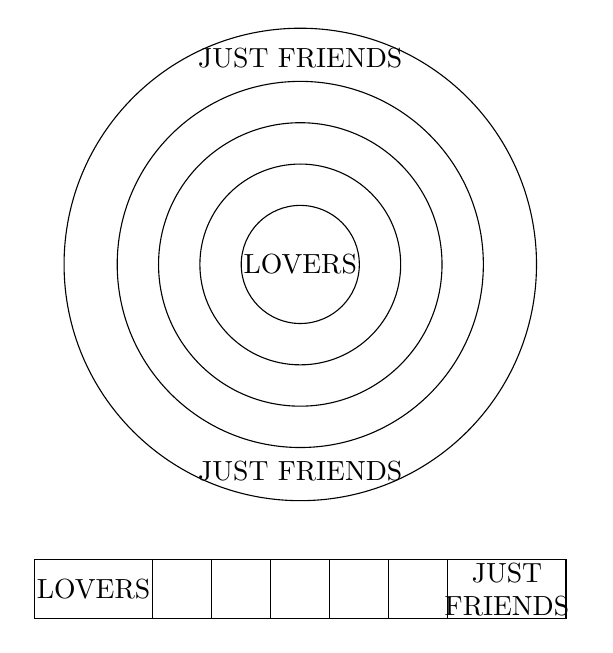
\begin{tikzpicture}[scale=0.75]
\begin{scope}
\draw circle (1) circle (1.7) circle (2.4) circle (3.1) circle (4.0)
  (0,0) node {LOVERS}
  (0,3.5) node {JUST FRIENDS}
  (0,-3.5) node {JUST FRIENDS};
\end{scope}
\begin{scope}[yshift=-5cm]
\draw
  (-2.5,0) rectangle +(-2,-1)
    +(-1,-0.5) node [anchor=center] {LOVERS}
  (2.5,0) rectangle +(2,-1)
    +(1,-0.5) node [text width=1.75cm,text centered] { JUST FRIENDS}
  \foreach \x in {-2.5,...,1.5} {
    (\x,0) rectangle ++(1,-1)
  }
;
\end{scope}
\end{tikzpicture}

\caption{Sample social combat map: Seduction}
\label{fig:social-combat-map-seduction}
\end{figure}

% \newpage


A seduction might be well modeled with a deep set of concentric circles --- say five or six --- with the objective of getting both characters in the bull's-eye (such as in \autoref{fig:social-combat-map-seduction}). Such an engagement could have multiple suitors and possibly require removing some or all from the map through Composure damage.

Suitors might be PCs or they might be NPCs or in some cases they might just be ``pawns'' --- if there is a concept you want to be relevant to the goal but that doesn't necessarily need to have free will in the fight, just give it a marker and no statistics. Players can move it around towards or away from goals (voters in an election or observers at a debate!) but it doesn't do anything on its own.

This could also be done with a simple linear track of, say, seven zones. Mark the first zone \LOVERS{} and the last zone \JUSTFRIENDS{}. Start the seducer on or near \LOVERS{} and the objective on or near \JUSTFRIENDS{}. Start other competitive suitors anywhere that seems fun or scary.

If the objective and anyone else are together on the \LOVERS{} zone, it has fallen for that suitor. If the objective and anyone else are together on the \JUSTFRIENDS{} zone, whoever has joined the objective there is removed from play.

% \newpage

\subsubsection{Debate}

\begin{figure}
\centering\footnotesize
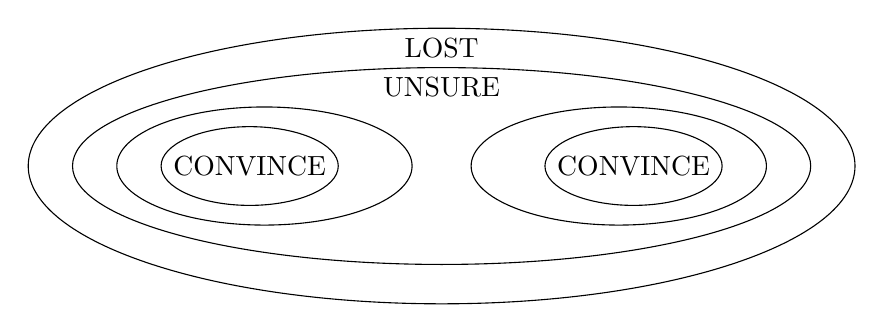
\begin{tikzpicture}[xscale=0.75,yscale=0.5]
\begin{scope}
\draw
  (-3,0) circle (2.5 and 1.5)
  (-3.25,0)   circle (1.5 and 1) node {CONVINCE}
  (0,0) ellipse (7 and 3.5) (0,3) node {LOST}
  (0,0) ellipse (6.25 and 2.5) (0,2) node {UNSURE}
  (3,0) circle (2.5 and 1.5)
  (3.25,0)   circle (1.5 and 1) node {CONVINCE}
%   (-3,0) node {CONVINCE}
%   (0,3.5) node {JUST FRIENDS}
%   (0,-3.5) node {JUST FRIENDS}
;
\end{scope}
% \begin{scope}[yshift=-5cm]
% \draw
%   (-2.5,0) rectangle +(-2,-1)
%     +(-1,-0.5) node [anchor=center] {LOVERS}
%   (2.5,0) rectangle +(2,-1)
%     +(1,-0.5) node [text width=1.75cm,text centered] { JUST FRIENDS}
%   \foreach \x in {-2.5,...,1.5} {
%     (\x,0) rectangle ++(1,-1)
%   }
% ;
% \end{scope}
\end{tikzpicture}

\caption{Sample social combat map: Debate}
\label{fig:social-combat-map-debate}
\end{figure}

% \newpage

A debate can be modeled with two sets of concentric circles representing opposing perspectives (see \autoref{fig:social-combat-map-debate}). The objective would be to move the opponent into your own central circle or moving the majority of audience members into your zone. Note that because of the steep drop-off in effectiveness at range, it will be necessary to move towards your opponent in order to engage him and pull him back to see your point (answering his specific arguments, showing sympathy and understanding).


\section{The Sequence}\label{sec:The Sequence}

Space combat is played in turns, each of which might represent fifteen to thirty minutes of in-game time --- this too has been largely abstracted. Each turn consists of several phases, and each phase will offer a test --- an opportunity to cross-compel, a roll, and an opportunity to tag and/or invoke \Aspects.

\subsection{Detection}
\label{sec:Detection}

% \makeatletter
% \newsavebox{\hbbox}%
% \begin{lrbox}{\hbbox}
% \begin{minipage}[c]{3.8cm}
% \sideboxtitle{Phases}
% The phases are:
% \begin{enumerate}
% \item Detection
% \item Position
% \item Electronic warfare
% \item Beam
% \item Torpedo
% \item Damage control
% \end{enumerate}
% \end{minipage}
% \end{lrbox}
% \begin{wraptable}{r}[\sidebarwidth]{0cm}\end{wraptable}
% \makeatother

% ~

\begin{wraptable}{r}[\sidebarwidth]{5cm}
\centering
% \begin{halfbox}{r}{5cm}{Phases}
\newsavebox{\hbbox}%
\begin{lrbox}{\hbbox}
\begin{minipage}[c]{4.5cm}
\sideboxtitle{Phases of space combat}
% The phases are:
\begin{enumerate}
\item Detection
\item Position
\item Electronic warfare
\item Beam
\item Torpedo
\item Damage control
\end{enumerate}
\end{minipage}
\end{lrbox}
\colorbox{sbbackground}{\usebox{\hbbox}}
% \caption{#5}
% \label{#6}
% \end{halfbox}
\end{wraptable}

Before a fight can start, everyone needs to find each other. Position is plotted on a linear scale from -4 to +4 on the map. As always, before any dice are rolled, the caller will ask for compels, at which time players can compel each other to fail to act. Failure to act in this case is represented by an automatic result of -4 (dice are not rolled and \Skills\ are not considered: your final result for your \Navigation\ check is -4).

A \Navigation\ check is rolled by each ship's navigation officer, and all rolls are ranked. Ties are resolved by raw \Navigation\ \Skill. The highest ranked Navigator will place two of the ships to be played on the map anywhere except the two most distant lines (-4 and 4). The next highest rank then places a single ship and this continues until all ships are placed. The lowest ranking Navigator places nothing. The ship which wins the detection round may also decide if there will be a positioning roll in the first turn (only). Once all the ships are placed, the winning ship in this phase decides whether to proceed to phase 1 or directly to phase 2. This allows a ship to attempt escape without engaging in combat immediately on being detected --- going to phase 1 --- or it allows it to use the tactical position from the detection phase for an optimized initial combat round --- going to phase 2.

In the event of a tie between two ships (as might happen when two standard T2 merchant ships meet, with default navigators), if neither ship is willing or able to invest fate points to gain victory, ships are placed randomly, based on a roll of the fate dice (it is only in this circumstance that a ship may begin at the 4 or -4 band).

\subsection{Position}\label{sec:Position} % \href{sec:id143}

As always, before any dice are rolled, the caller will ask for compels, at which time players can compel each other to fail to act. Failure to act in this case is represented by an automatic result of -4 (dice are not rolled and Skills are not considered: your final result for your positioning check is -4).

Spacecraft positions are plotted on a simple linear scale from -4 to +4. Ships begin as they were placed in the detection phase. At the beginning of each round of combat, pilots jockey for position. All pilots roll their ship's V-shift rating limited by their effective Pilot Skill (i.e. if one character is serving both as Navigator and Pilot, then the Pilot's effective Pilot Skill is reduced by one). Note also that this is not simply a modifier to the roll: since V-shift is limited by effective Pilot Skill, this penalty might affect performance for the first turn as well.

In addition, ships may apply burn: by running their drives over rating, they can exchange Heat for an advantage in maneuver, improving the V-shift roll. Any ship may declare that it is applying burn, state the value and add that value to their roll (not to the V-shift rating). They immediately take a hit to their Heat stress track equal to the value of their burn, marking that box and all unmarked boxes below it. If the highest box to be marked is already marked, mark the next higher open box. Before marking the damage to the Heat stress track, the pilot may reduce the detrimental effects through Consequences exactly as mitigating combat damage. The caller may allow negotiation of burn declarations at his preference, though generally a declared burn rating by a ship's player must stand.

Ships may choose not to use their drives in order to bleed heat. Each turn that the V-Shift is not engaged allows the highest filled box in the Heat track to be cleared immediately. This decision results in an automatic -4 final result for the positioning check, which might still be modified by Aspects, but no dice are rolled and no Skill is used. No burn declarations can be made once the caller declares the bidding closed and asks for dice on the table.

Only the highest roller may alter any ship's positions:
\begin{itemize}
\item He may move himself the difference between his roll and the lowest roll, or
\item He may move any ship with a lower roll up to the level of the
difference between them.
\end{itemize}

He may not, however, move any vessel more map bands than his own vessel's V-shift rating. Remember, moving a ship between the 3 and 4 bar (or the -3 and -4) costs 2 shifts, and moving a ship from the last bar off the map costs 3 shifts.

If the winning positioning roll is tied, the next highest roll is the winner. This presents some interesting tactical choices for fate point expenditure: sometimes it's advantageous to forfeit your awesome roll so that your ally, who rolled lower, can make use of his better V-shift, for example. You might then use an Aspect to force a tie so that you lose control.

If a ship exceeds the band at -4 or 4, they leave combat, whether forced off by others or maneuvered off by their own pilots. In this fashion a really excellent pilot in a hot ship can cut down the odds by positioning enemy vessels off the map until he faces only one opponent. Similarly, more than two ships chasing a single ship can usually keep the lone opponent on the map through positioning.

\subsection{Electronic Warfare}\label{sec:Electronic Warfare}
\vfil
As always, before any dice are rolled, the caller will ask for compels, at which time players can compel each other to fail to act. Failure to act in this case is represented by the ship being unable to declare a target.

Before any destructive weapons are used, each ship may conduct electronic warfare, pitting its communications officer against the enemy. If a communications officer has \stunt{Military-grade Communications}, she may pick a target and roll the ship's \skill{Electronic Warfare} (EW) rating, amplified by her effective \skill{Communications} Skill (if the communications officer has acted in any of the previous phases, there is a cumulative -1 penalty for each phase she has acted). The defender also makes a roll, of his ship's \skill{EW} rating, amplified by the communications officer's effective \skill{Communications} Skill. The rating may be zero, in which case there is there is no crewman staffing the position unless this is done by one of the PCs. Ships may have a Stunt (\stunt{Firewall}) that automatically provides a defense value of 2, and which may not be modified. Subtract the defender's modified roll from the attacker's.

As with any roll, these results can now be modified by tagging or invoking \Aspects\ and paying a fate point to get +2 or re-roll.

Positive values are treated as shifts against the defender, and
%
negative values are treated as shifts against the attacker.
%
Whoever has shifts against him will take a \Data\ stress track hit to the ship. Before damage is calculated, the player may apply \Consequences\ to reduce the number of shifts: a mild Consequence reduces the shifts by one, a moderate Consequence reduces the shifts by two, and a severe Consequence reduces the shifts by four. Recall that no entity can have more than three Consequences of any kind and never more than one of each type.

% \newpage

Once the final number of shifts are determined, the corresponding box on the \Data\ stress track is marked and all open boxes below it are also marked. If the highest box to be marked has already been marked, mark the next highest open box.

Note that only one roll is made for each ship, so in some cases with more than two ships in play, a single roll may defend against multiple attacking rolls as well as conceivably acting as the attacking roll on a declared target. Note also that a good defense against hacking can inflict damage on the attacking \Data\ stress track, even if the defending communications officer does not have Military-grade \skill{Communications}.

The Electronic Warfare (EW) defense roll is persistent through this phase, but the total may be added to over the course of the phase through the spending of fate points. An outnumbered ship may still mount a reasonable defense.

% \newpage

\subsection{Beam Weapons}\label{sec:Beam Weapons} % \href{sec:id145}

Beam weapons subsume all relatively short range unguided weaponry, so they may be described as lasers of various wavelengths, artillery, rockets, railguns, electromagnetically propelled storms of small projectiles, particle beams, or anything else that suits the setting developed at the table. Beams are used both offensively, to directly damage targets at shorter ranges, and defensively, to defend against torpedoes (see Torpedo phase for details).

As always, before any dice are rolled, the caller will ask for compels, at which time players can compel each other to fail to act. Failure to act in this case is represented by a failure to declare a target in whatever phase the player ship was compelled.

A ship with a Beam Skill can attack at any value from 1 up to the full Beam rating. When Beams are fired offensively the attacker must declare what Beam rating he will apply. Note the Beam value used, as it will be relevant in the Torpedo phase.

All combat rolls are made at the Beam rating amplified by the gunner's Gunnery Skill (that is, the Beam rating is used and increased by one if the Gunnery Skill is higher). If the gunnery officer has acted in any of the previous phases, there is a cumulative -1 penalty to the effective Skill level for each phase he has acted. 

Beams firing at three or more bands range subtract 2 from the roll. Attacks are resolved as they are declared, again leveraging social pressure to determine who goes first: the caller closes the call for targets by announcing a final call, and counting slowly to three (if necessary --- if your caller is fair and fun, he'll leave plenty of time), after which no further targets can be announced.

There is no skill to defend against Beams. A roll with no modification is made to oppose all incoming Beam attacks. Ship's may have a Stunt (Vector Randomizer) that changes the base from 0 to 2.
Defensive rolls are made once for each defensive system but stay on the table --- that defensive roll you made against Beams stands throughout the Beam Weapons phase, complete with any modifications from invoking Aspects, using spin, etc. Defensive rolls are persistent through the phase, so it can be handy to note them on the ship card or use a coloured 12- or 20-sided die set to the result. Sometimes we write them on the map. Offensive Beam rolls are distinct from defensive Beam rolls (from the Torpedo phase) and should be recorded separately.

% \newpage

Subtract the defender's final sum from the attacker's to find the number of shifts, and thus the amount of stress on the defender's \Frame\ track. The defender may reduce these by applying one or more Consequences:
\begin{itemize}
\item reduce the shifts by one by applying a mild Consequence
\item reduce the shifts by two by applying a moderate Consequence
\item reduce the shifts by four by applying a severe Consequence.
\end{itemize}

Recall that no entity may have more than three Consequences and never more than one of each kind.

% \newpage

\subsection{Torpedoes}\label{sec:Torpedoes} % \href{sec:id146}

As always, before any dice are rolled, the caller will ask for compels, at which time players can compel each other to fail to act. Failure to act in this case is represented by a failure to declare a target in whatever phase the player ship was compelled.

Torpedoes attack at the spacecraft's Torpedo Skill rating, amplified by the gunner's effective Gunnery Skill (that is, the Torpedo rating is used and increased by one if the effective Gunnery rating is higher). If the gunnery officer has acted in any of the previous phases (including the Beam phase), there is a cumulative -1 penalty for each previously active phase.

Torpedoes firing at one or zero bands range subtract 2 from the roll. Attacks are resolved as they are declared, again leveraging social pressure to build an initiative order as in the Beam phase. The caller closes the call for targets by announcing a final call, and counting slowly to three, after which no further targets can be announced.

A Beam roll is made to oppose all incoming Torpedoes. To do this, the beam position must be staffed. If Beams were fired in the Beam Weapons phase, then the roll may be made as usual, amplified by gunner's effective Gunnery Skill. If Beams were not fired, then there must be a trained crew member available to man the beams in this phase: normal penalties and bonuses apply, but since each crew member may only act once per phase, a ship with a single gunner (as might happen with a skeleton crew) may have to choose between offensive Torpedo fire and defensive Beam fire. Beams so used may also have been fired offensively, and defensive fire may cause damage to the Heat stress track. Ships with no Beam rating or those unwilling to fire Beams defensively, roll with a base of 0 unless they have a Stunt (Point Defense) that changes the base from 0 to 2.

Defensive rolls are made once for each defensive system but stay on the table --- that  defensive roll you made with the Beams stands throughout the Torpedo Phase, complete with any modifications from Aspect invocation, spin, or other sources. As these rolls are persistent through the phase, it can be handy to note them on the ship card or use a coloured 12- or 20-sided die set to the result. Sometimes we write them on the map. Though persistent, defensive rolls are distinct from offensive rolls and should be recorded separately.

% \newpage

When Beams are fired defensively the attacker must declare what Beam rating he will apply. He may apply any value from 0 to the full Beam rating. Note the Beam value used. If the sum of the offensive Beam used in the Beam phase plus the defensive Beam used in the Torpedo phase is greater than the total Beam rating, then the ship takes a hit on the Heat stress track equal to the difference and marks all boxes below as well.

Subtract the final defender's sum from the attacker's to find the number of shifts, and thus the amount of stress on the defender's \Frame\ track. The defender may reduce these by applying one or more Consequences:
\begin{itemize}
\item reduce the shifts by one by applying a mild Consequence
\item reduce the shifts by two by applying a moderate Consequence
\item reduce the shifts by four by applying a severe Consequence.
\end{itemize}

Recall that no entity may have more than three Consequences, nor more than one of each kind.

% \newpage

\subsection{Damage Control}
\label{sec:Damage Control}

Damage control checks may now be made on Frame stress tracks (using one crew member's effective \skill{Engineering} Skill) or Data stress tracks (using one crew member's effective \skill{Computer} Skill). Since each crew may only staff one position per phase, the same individual may not be responsible for both rolls. If the engineer or computer officer has acted in any of the previous phases, there is a cumulative -1 penalty for each previously active phase. The target number for success is the highest box marked on the relevant track. The number of successes indicate the track box that can be erased. Erase it and all unmarked boxes below it.

The Heat stress track cannot be repaired during combat, except by shutting off engines, as described in the positioning phase.


\section{Damage}\label{sec:social-combat-damage}

Stress box hits are not real damage, but they can lead to Consequences. All stress box hits are removed after a few days of relaxing stress-free downtime. As with personal combat, the table should rule when enough time has passed or whether the downtime was sufficiently relaxing. Generally speaking it should be trivial.

\subsection{Recovering Consequences}\label{sec:social-combat-recovering-consequences}

A mild Consequence can be self-medicated with a bottle and some time alone once the scene is over. No roll is required and it is cleared as soon as the social combat scene is over.

A moderate Consequence remains until the end of the session in which it was incurred.

A severe Consequence must be carried through one complete session in which the associated stress track is never marked. If it is incurred during session one, it is gone no sooner than the end of session two, and if the associated stress track takes hit in a fight during that session, you'll need to hold the Consequence through yet another one.



% \vfil
\chapter{Platoon Combat}
\label{cha:platoon-combat}
% \vfil

\begin{sidebox}{Military Organization}

Organizational units vary from army to army, and from world to world, but it might help to think in terms of the following:

\begin{description}
\item [A team] is composed of 2-5 soldiers of a single vehicle. This is the basic unit of platoon-scale combat, and is represented on the map by a single figure.

\item [A squad] is composed of 1-3 teams and is commanded by a Sergeant or a Corporal.

\item [A platoon] is composed of 2-6 teams, commanded by a Lieutenant.

\item [A company] is composed of 3-5 platoons, under the command of a Captain. This is the largest unit to be controlled by a single player.

\item [A battalion] is composed of 2-6 companies, under the command of a Lieutenant Colonel. An engagement of two battalions is at the extreme upper end of the size of what can be modeled in Platoon-scale combat in Diaspora.
\end{description}
\end{sidebox}
% \vfil


The rules for platoon-scale wargaming are provided in Diaspora for campaigns that want to focus on military combat. Perhaps the players are old army buddies, offering their services to their planet's defense. Perhaps a heavily balkanized world is enlisting off-worlders to fight their battles for them. Perhaps the characters are a mercenary strike team, performing short-term contracts for anyone willing to pay. Whatever the story, it is easy to imagine combats where the scale of personal combat is simply inadequate: when there are too many individuals active in battle, platoon scale provides opportunities for incorporating infantry, artillery, armour and aircraft units in a ground war.

% \vfil

Some campaigns may choose to build around this sort of encounter, with the story effectively moving the characters from one mercenary ticket to the next with each game session. Others might never need these rules, but will be able to occasionally use them to model robbing an armoured vehicle.
%
% \vfil
\iflandscape{\newpage}{}

%
Whatever the application, the rules are provided as a means of representing something that could also be done within the existing Diaspora mechanisms. Operating at the platoon scale becomes an option that is available for those tables that want it.

% \vfil

The organizational unit of interest is the platoon. This is a number of single units, one of which is a leader, all in communication. The only stress track used is the \Morale{} stress track of individual units.

For infantry units, platoon scale represents combat between teams of 2-5 soldiers organized into platoons of 2-6 teams; an armour platoon might be 4 or 5 tanks. Individual characters can improve a platoon's performance, but, as in space combat, an individual can only modify the performance of the larger unit. The principles of FATE still apply, of course, and (as is common in Diaspora), they have been stripped down.

At the platoon scale, there is only a single stress track: \Morale. If a platoon loses morale, it can no longer function. Whether it has lost morale because of its ongoing frustration with lack of supply lines, because of the constant pressure of close enemy fire, or simply because most of the platoon has been killed, Diaspora models the only crucial variable of loss at the platoon scale along the axis of morale.

In most games, players will control either a single platoon, or (as is more usual when used as a stand-alone game) a company of 3-5 platoons.

As with the other mini-games, platoon-scale war-gaming can be played independent of the larger Diaspora RPG.

% \vfil
% \newpage

\section{The Map}\label{sec:social-combat-map}
% \vfil

Social combat takes place on a zone map much as it does with personal combat. Instead of representing some physical geography, the map represents the social space of the encounter. Because of the kinds of options available to characters involved in social combat, certain kinds of map shapes have certain kinds of effects on behaviour and can be used to represent specific issues.

In general, concentric circles imply intimacy. Zone shapes with many borders, and therefore many avenues of escape and access, better represent socially open places like chatting about the weather at a party. Intimate zones are often objectives, such as when you want to get someone to reveal valuable information, and so you want to maneuver them into intimate, trusting conversation.

% \newpage

To begin with, moving between zones has no additional cost --- there is no initial use of ``borders'' as there is in personal combat. Characters in the same zone can be said to be engaging each other socially: they are conversing about interesting, relevant things that they care about. Conversely, the further apart characters are on the map, the more social distance is in their conversation. Range has a deep impact on the effectiveness of characters' interactions and so one must usually close the range before one can do anything useful, such as move the conversation to a more intimate space.

% \newpage

Zones represent in the first instance a degree of intimacy in the social context. This will sometimes correspond to a spatial dimension too, but more often it represents something much more nebulous. For instance, a separate zone might correspond to a small balcony where a conversation might occur. It is often a good idea for the table to design the map of the social combat as a group.

Optionally, once the map is created, each player may choose to place one free-taggable \Aspect{} on a single zone, or a pass value of 2 on a single border, to reflect the personal contours of the social situation.

% badbox here
% \newpage

\subsection{Time}\label{sec:Time}

For each zone on the map, create one time box to represent available time to resolve. If you need to know exactly how long something took, the table should determine the maximum amount of time something is allowed (even the best party will disperse by morning). If a victory condition is achieved before the time boxes run out, the maximum time can be downgraded a number of shifts on the Time Track (Dealing With Time, Chapter 2) equal to the number of unchecked boxes. Often, table consensus will determine a very similar result in any case.

% \newpage

\subsection{The Actors}\label{sec:The Actors}

One of the biggest conceptual hurdles in adopting this system for resolving social interactions is recognizing that not every person in a scene needs to be represented on the map. Part of this is embodied within the zones themselves, as \Aspects{} on the zones can represent the other people involved.

This can in fact be made even more abstract, when you want to make a situation tactical that has become mired or unproductive in regular role-play. By making some of the actors on the map ideas instead of explicit people, you can conduct a scientific investigation or any other information-revealing multi-step endeavour. Make the opposition the Fact and, maybe, an Attractive Falsehood and you can do science. Add in people with conflicting goals (a young whipper-snapper who wants to be primary author on the publication of your discovery!) and the abstract can engage the concrete in both directions.

% \newpage

\subsection{Victory}\label{sec:Victory}

Victory conditions should relate to map position. Usually the objective will be to get a certain person or persons into a specific zone before the timer runs out. This can be more complex, however, to achieve different goals: if you want to model persuading a crowd, you could score participants by how many crowd members are in their target zone when the timer runs out. Feel free to push the system around and find other victory conditions.

\newpage

\subsection{Sample Maps}\label{sec:Sample Maps}

% \newpage

\subsubsection{Party}

A party has a lot of accessible conversation space --- everyone is there to chit-chat after all --- and probably at least one intimate space. It is well represented by a central shape with several attached shapes. Inside one attached space, add a couple of concentric circles for intimacy. An objective in the party might be to hook up with a powerful businessman and get him to brag about his company's secret operation on the dark side of the moon: you win if you can get him, yourself, and the science officer into the center of the intimate zone before the timer runs out.

The party map doesn't need to be complicated --- the simpler it is the faster things will go. The important thing is to make it take a few steps to get to the target zone and be complex enough to imply story with every move. The map above is about the minimum complexity you would want from a social combat map. It might be close to the maximum also!

% \newpage

\subsubsection{Seduction}

\begin{figure}
\centering\footnotesize
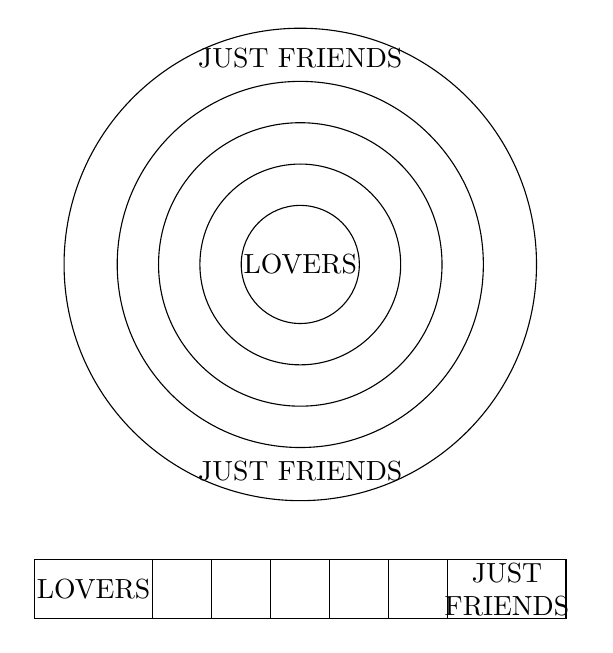
\begin{tikzpicture}[scale=0.75]
\begin{scope}
\draw circle (1) circle (1.7) circle (2.4) circle (3.1) circle (4.0)
  (0,0) node {LOVERS}
  (0,3.5) node {JUST FRIENDS}
  (0,-3.5) node {JUST FRIENDS};
\end{scope}
\begin{scope}[yshift=-5cm]
\draw
  (-2.5,0) rectangle +(-2,-1)
    +(-1,-0.5) node [anchor=center] {LOVERS}
  (2.5,0) rectangle +(2,-1)
    +(1,-0.5) node [text width=1.75cm,text centered] { JUST FRIENDS}
  \foreach \x in {-2.5,...,1.5} {
    (\x,0) rectangle ++(1,-1)
  }
;
\end{scope}
\end{tikzpicture}

\caption{Sample social combat map: Seduction}
\label{fig:social-combat-map-seduction}
\end{figure}

% \newpage


A seduction might be well modeled with a deep set of concentric circles --- say five or six --- with the objective of getting both characters in the bull's-eye (such as in \autoref{fig:social-combat-map-seduction}). Such an engagement could have multiple suitors and possibly require removing some or all from the map through Composure damage.

Suitors might be PCs or they might be NPCs or in some cases they might just be ``pawns'' --- if there is a concept you want to be relevant to the goal but that doesn't necessarily need to have free will in the fight, just give it a marker and no statistics. Players can move it around towards or away from goals (voters in an election or observers at a debate!) but it doesn't do anything on its own.

This could also be done with a simple linear track of, say, seven zones. Mark the first zone \LOVERS{} and the last zone \JUSTFRIENDS{}. Start the seducer on or near \LOVERS{} and the objective on or near \JUSTFRIENDS{}. Start other competitive suitors anywhere that seems fun or scary.

If the objective and anyone else are together on the \LOVERS{} zone, it has fallen for that suitor. If the objective and anyone else are together on the \JUSTFRIENDS{} zone, whoever has joined the objective there is removed from play.

% \newpage

\subsubsection{Debate}

\begin{figure}
\centering\footnotesize
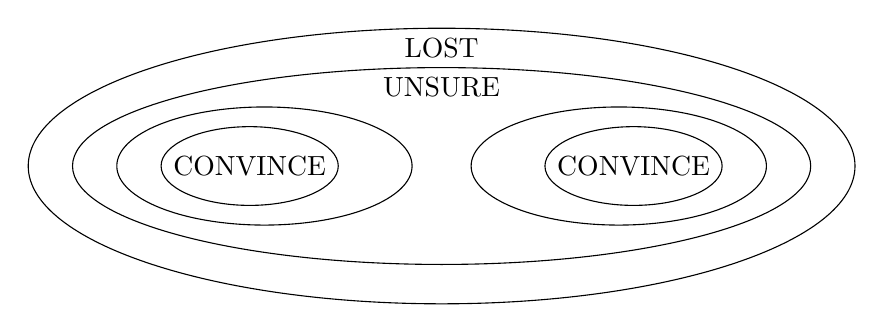
\begin{tikzpicture}[xscale=0.75,yscale=0.5]
\begin{scope}
\draw
  (-3,0) circle (2.5 and 1.5)
  (-3.25,0)   circle (1.5 and 1) node {CONVINCE}
  (0,0) ellipse (7 and 3.5) (0,3) node {LOST}
  (0,0) ellipse (6.25 and 2.5) (0,2) node {UNSURE}
  (3,0) circle (2.5 and 1.5)
  (3.25,0)   circle (1.5 and 1) node {CONVINCE}
%   (-3,0) node {CONVINCE}
%   (0,3.5) node {JUST FRIENDS}
%   (0,-3.5) node {JUST FRIENDS}
;
\end{scope}
% \begin{scope}[yshift=-5cm]
% \draw
%   (-2.5,0) rectangle +(-2,-1)
%     +(-1,-0.5) node [anchor=center] {LOVERS}
%   (2.5,0) rectangle +(2,-1)
%     +(1,-0.5) node [text width=1.75cm,text centered] { JUST FRIENDS}
%   \foreach \x in {-2.5,...,1.5} {
%     (\x,0) rectangle ++(1,-1)
%   }
% ;
% \end{scope}
\end{tikzpicture}

\caption{Sample social combat map: Debate}
\label{fig:social-combat-map-debate}
\end{figure}

% \newpage

A debate can be modeled with two sets of concentric circles representing opposing perspectives (see \autoref{fig:social-combat-map-debate}). The objective would be to move the opponent into your own central circle or moving the majority of audience members into your zone. Note that because of the steep drop-off in effectiveness at range, it will be necessary to move towards your opponent in order to engage him and pull him back to see your point (answering his specific arguments, showing sympathy and understanding).


\section{Command}\label{sec:Command}

\index{command range}
A platoon is a grouping of units that can be ordered to act by a leadership unit. By default that unit must be in the same zone as the leader, but this may be modified by Stunts. The maximum distance allowed between a unit and its leader in order to maintain membership in the platoon is the unit's command range.
%TODO glossary: command range

\rulebox{Command range indicates how may zones a unit can be away from its leader and still be in communication with it.}

\index{OOC|see{Out Of Communication}}\index{Out Of Communication (OOC)}
Command range is zero (same zone only) unless modified by a stunt on the leader, the unit, or both. Non-leader units that do not belong to a platoon (are out of command range) may move away from enemy units, may attack enemy units that have fired upon them, and may attempt to unjam and remove Out Of Communication (\OOC) counters on themselves, but may take no other actions. They have no fate points and do not share a platoon's Consequences. Hits on these units may not be mitigated by a platoon taking a \Consequence. Units that become disassociated from their platoon do not change the platoon's fate point total.

Platoon membership is checked at the beginning of the platoon's action. Units with \OOC{} counters are only part of a platoon membership when in the same zone as the leader unit.

A leader unit with \OOC{} counters disconnects all its platoon members but suffers none of the other restrictions described here.


\section{Units}\label{sec:Units}
\iflandscape{\vfil}{}


A unit is the minimum element represented on the map for each type: a single miniature or counter. For infantry, that's a team of a few soldiers. For armour that's one vehicle. For artillery that's a battery.

There are four types of team units: infantry, artillery, armour, and aircraft. For each platoon, one unit (which may not be aircraft) is also designated the leader. There is no maximum number of units in a platoon.

Each unit in a platoon grants the platoon one fate point. All fate points are kept on the platoon and spent from the platoon. All Consequences are on the platoon.

Similarly, spin counters are associated with platoons and not with units. They may be spent by any unit in the platoon. Spin expires after having had one complete turn in which to use it (thus if spin is acquired during a defensive roll, it lasts until the end of the platoon's next opportunity to act whereas if it is acquired during movement, say, it lasts until the end of the platoons next opportunity to act and not the opportunity in which it moved).

Units that are not normally part of a platoon (typically aircraft) are associated with a particular platoon and donate their fate point to that platoon. They draw fate points from that platoon when invoking, tagging, or compelling.

All units have Skills, Aspects, Stunts, and a \Morale\ stress track. Skills are an n-cap pyramid (i.e. one Skill at level three, two Skills at level two, and three Skills at level one) or a column (i.e. one Skill at level four, one Skill at level three, one Skill at level two, and one Skill at level one).

All units have one Aspect and contribute one fate point to their platoon. Infantry units have a baseline of zero Stunts, plus one Stunt for each technology level. All other units have one Stunt, plus one additional Stunt for each technology level; consequently, units at T-1 or lower do not have Stunts. As described below, the platoon leader always has one additional Stunt, regardless of technology level. No unit may have negative Stunts.

Units have only one stress track: \Morale. When a unit takes a hit past the end of its \Morale\ track that cannot (or will not) be mitigated by a platoon \Consequence, it is eliminated. The narrative associated with this elimination can be determined by the table: it might represent panic and dispersal or surrender; a complete lack of morale is also adequately explained by everyone being killed. Some combination of the three is most likely.  The mechanical effect at this scale is the same. As with other stress tracks, a hit on a marked box rolls up to the next unmarked box.

\subsection{Skills}
\label{sec:platoon-combat-skills}

All Skills are eligible to be chosen by any unit type. See \autoref{tab:platoon-unit-skills} for a list of the unit skills available.

\input{tables/platoon-unit-skills}

Units may only roll Skills for which they are trained. The only
exception is when defending against an opposed roll, in which case the
untrained Skill is presumed to be zero. The only case presented here
is Armour, though with an appropriate Stunt  Camouflage may also
qualify.


% \subsection{Unit Stunts} % should be?
\subsection{Stunts}\label{sec:unit-stunts}
\begin{description}
\item[Cavalry]
this unit is undersized and overpowered, so its maximum move is increased by one (infantry, armour, or artillery only). Infantry units may take this \Stunt\ multiple times: the unit may be thought to have an intrinsic vehicle for mobility. When taken by an armour unit, the \Stunt\ is designated ``\stunt{Light}.''

\item[Special forces]
this unit is not automatically spotted when it shares a zone with an enemy unit (infantry only).

\item[Wireless]
unit is attached to an integrated communications net, increasing command range by 1. May be taken multiple times.

\item[Engineer]
may use a successful maneuver roll to use up the free-tag on an enemy-applied \Aspect\ or make two maneuver rolls on the zone it is in instead of the usual one (infantry and armour only).

\item[Guerrilla tactics]
attacks from this unit never generate spin for the defender (infantry only).

\item[Highly trained]
this unit has one additional morale box.

\item[Infantry carrier]
this unit can carry infantry (armour or aircraft only). One infantry unit in the zone can move with this carrying unit (including traversing the Re-arm track for aircraft). The infantry unit cannot act this turn (before or after the move). The unit can begin the game carrying its infantry load. For aircraft, when the aircraft re-enters the map, the infantry is deployed and may act normally; the aircraft may not otherwise act while deploying infantry. Carried infantry do not have to be in the same platoon as the carrier.

\item[Interceptor]
if this unit is on the LAUNCH! box, it may enter the map any time an enemy aircraft enters the map and act immediately before the target aircraft can act. It may act only against this target aircraft (aircraft only).

\item[Irregulars]
this unit is an irregular non-professional unit (a sink \Stunt, chosen only to model a unit that is less effective than other units of the same technology level). Other sink \Stunts\ can be invented to fit the scenario: \stunt{Slow}, to represent a low rate of fire, etc.

\item[Long range]
ignores one zone for attack roll range modification. May be taken multiple times.

\item[Orbital]
this unit can only be attacked by fire from other orbital units (artillery only). Orbital units that are attacked with the jam action, however, take damage as though attacked with weapons (in addition to the effects of jamming).

\item[Prepared positions]
this unit was set up long before the battle (artillery only). Before combat begins, it may add a the \Aspect\ of \aspect{Locked in} to any two zones on the map. This \Aspect\ can be free-tagged by any allied artillery unit, and remains an \Aspect\ on the zone which may be tagged normally thereafter.

\item[Scatterable mines payload]
this unit can deliver area-denial ordnance (ie, mines). Pass values placed by the unit from an interdiction strike are permanent (artillery and aircraft only).

\item[Scout]
this unit can continue movement after entering a zone containing enemy units (infantry and armour only).

\item[Skill substitution]
With an appropriate narrative, additional \Stunts\ may be designed to allow \Skill\ substitutions. Each unit may only ever have one \Skill\ substitution \Stunt. The following are offered as representative examples.

\begin{description}
\item[Agile]
can use \skill{Movement} in place of \skill{Armour} (armour only).

\item[Graphite payload]
this unit can deliver payloads designed to interrupt electrical and electromagnetic function (artillery and aircraft only).  It may use its \skill{Indirect Fire} Skill to effect Jam attacks (which would normally use the \skill{Signals}). Note that this can be combined with \stunt{Zone Effects} to jam all units in a zone (regardless of owner).

\item[Shoot and scoot]
this weapon system is designed to be fired while on the move or to move very soon after firing a mission. It may use its \skill{Movement} Skill instead of \skill{Camouflage} (artillery only).

\item[Technology enhancement]
increase any \Skill\ by one. This \Stunt\ may be taken at most twice per \Skill, for a total bonus of +2.

\item[Stealth technology]
designed to hide, this unit can use \skill{Camouflage} in place of \skill{Armour} (armour only).
\end{description}

\item[VTOL]
this unit is designed to stay on target --- once on the map it may remain, moving a maximum of 1 zone (its free move) per turn (aircraft only).

\item[Zone effects]
this unit may attack all units in the target zone with one roll at -2 (armour, artillery, or aircraft only). Units do not need to be spotted to be attacked in this fashion.
\end{description}

\subsubsection{Leadership stunts}

Each platoon leader additionally chooses one of the following four Stunts.

\begin{description}
\item [Battlefield genius]
units can be one zone further from the Leader than otherwise allowed.

\item[Logistics genius]
units in platoon do not have the \aspect{Out of ammo} Aspect.

\item[Tactical genius]
units in platoon ignore one extra zone of range when attacking.

\item[Not a genius]
sink Stunt for crap commanders.
\end{description}


\subsection{Stress Tracks}\label{sec:platoon-unit-stress-tracks}

All units have a single stress track, \Morale. A platoon may expend \Consequences to mitigate hits past the end of the track on a unit. A platoon has three \Consequences\ to allocate and each can mitigate two shifts. As is standard in FATE, a platoon \Consequence\ becomes an Aspect and may be free-tagged once or compelled or tagged normally to affect any unit in the platoon.

\begin{itemize}
\item Infantry units have a base \Morale\ stress track of two boxes.
\item Armour units have a base \Morale\ stress track of one box.
\item Artillery units have a base \Morale\ stress track of two boxes.
\item Aircraft units have a base \Morale\ stress track of one box.
\end{itemize}

Unit \Morale\ tracks are modified by the unit's \Veteran\ skill. Leader units also gain a bonus \Morale.

\begin{itemize}
\item Leader units increase the base \Morale\ stress track by two.
\item Units with Veteran 1 or Veteran 2 increase their \Morale\ stress track by one.
\item Units with Veteran 3 or Veteran 4 increase their Morale stress track by two.
\item Units with Veteran 5 or Veteran 6 increase their Morale stress track by three.
\item Some stunts may further alter the length of the Morale stress track.
\end{itemize}


\subsection{Aspects}
\label{sec:platoon-unit-aspects}

All units have one descriptive Aspect chosen by the owner and add one fate point to their platoon. All units also have the Aspect \aspect{Out of ammo}. A unit, when spending fate points, expends platoon fate points. When a unit gains a fate point through a compel, that fate point belongs to the platoon.


\subsection{Infantry}
\label{sec:Infantry}

% \input{C08/TB-infantry}

Infantry units represented a small number of individuals of similar or concerted equipment: a unit typically represents 2-5 individuals, though it could be as many as 12. Specific weapons and armour per individual are not modelled except as they are represented in the Skill and Stunt list.

Infantry have a 3-cap Skill pyramid. Infantry units choose one Skill at rank 3, two Skills at rank 2, and three Skills at rank 1. They have a Morale track two boxes long. If the unit has Veteran at rank 1 or 2, the Morale track is three boxes long. If the unit has Veteran at rank 3, the Morale track is four boxes long.

The maximum movement for infantry is two zones. Infantry units may move a maximum of two zones regardless of their movement roll.


\subsection{Armour}
\label{sec:armour}

Armour units are individual tanks, cars, or other mobile armoured platform. They represent all of the equipment present on precisely that model of vehicle.

Armour has a 4-cap Skill column. Armour units have one Skill at rank 4, one at rank 3, one at rank 2, and one at rank 1. They have a Morale track one box long. If the unit has Veteran Skill 1 or 2, the Morale track is two boxes long. If the unit has Veteran Skill of 3 or 4, the Morale track is three boxes long.

The maximum movement for armour is four zones. Armour units may move a maximum of four zones regardless of their movement roll result.


\subsection{Artillery}
\label{sec:Artillery}

Artillery units are equipment capable of Indirect Fire which are kept off map. They move only in a notional sense insofar as they can roll Movement as a defensive roll against counter-battery detection and Indirect Fire. Infantry-based artillery (such as mortar or grenade launcher crews) should be represented by including an Indirect Fire Skill on an infantry unit. Artillery batteries that need to be represented on the map for purposes of the scenario should be represented by their attending personnel as lightly armed infantry units.

It can be handy to create an off-map artillery card for artillery platoons, especially if they have a command range greater than one. This will greatly simplify aircraft attacks on the artillery platoon. Artillery has a 3-cap Skill column. Artillery units have one Skill at rank 3, one at rank 2, and one at rank 1. Their Morale track is two boxes long. If the unit has Veteran Skill 1 or 2, the Morale track is three boxes long. If the unit has veteran Skill 3, then the Morale track is four boxes long.

Artillery may make Movement rolls to change position on their battery
card if there is more than one zone on the card. Moving artillery
units do not remove \SPOTTED\ markers, however.

Artillery can only fire on targets that are in line-of-sight to a
friendly unit that is currently attached to a platoon (or does not
need to be) and has no Out Of Communications (\OOC) counters.

All artillery units in the same platoon are considered to be in the
same zone as their leader for purposes of command and communication,
and for purposes of any attacks that affect all targets in a single
zone when attacked by aircraft, unless they have a Stunt that allows a
greater command range. All members of an artillery platoon not
situated on the map must be on the same artillery card (they cannot be
spread over multiple cards). Not all units in an artillery platoon
need to actually be artillery units (there might be an infantry leader
unit supplying comms and other coverage and an armour unit supplying
AA for example).
Non-artillery units in an artillery platoon must be in the off-map
artillery card in order to be associated with the platoon. This means
that, although the leader unit might be represented by something other
than artillery (an armour or infantry unit might be more advantageous)
it will gain no advantages from its mobility on the map.


\iflandscape{}{\vfil}
\subsection{Aircraft}
\label{sec:Aircraft}

Aircraft are independent units and therefore require no leader unit. They also move differently from other units: an aircraft unit may place itself on any zone on the map when its turn to act comes up.

Aircraft are automatically spotted when they are on the map.

Aircraft movement is different from other units:

Aircraft begin on the \LAUNCH\ box of the Re-arm track.

While on the Re-arm track, an aircraft unit may make Movement rolls to pro\-gress along the track.

An aircraft on the \LAUNCH\ box at the beginning of its turn may be placed on any zone on the map. Its turn is now over.

Once an aircraft acts while on the map (usually in the turn after it has moved there), it is returned to the RE-ARM box of the Re-arm track.

An aircraft unit on the map may act as any other unit except that it may not make a Movement roll.

Aircraft have a 4-cap Skill column. Aircraft units have one Skill at rank 4, one at rank 3, one at rank 2, and one at rank 1. They have a \Morale\ track one box long. If the unit has \Veteran\ Skill 1 or 2, the \Morale\ track is two boxes long. If the unit has \Veteran\ Skill 3 or 4, then the Morale track is three boxes long.

The maximum movement for aircraft is zero zones as they are not represented on the map. Aircraft units do not move on the map in the same fashion as ground units and so do not make Movement rolls except to decrease their re-arm time.

Aircraft increase range by 1 for all distance calculations (both against them and against other targets).

Aircraft can only be attacked by the Anti-air Skill.


\subsection{Leadership}
\label{sec:Leadership}

Each platoon has one, and only one, leader unit. An infantry, armour, or artillery unit can be designated a leader.

A leader unit may perform a  action in addition to its normal action. It may, therefore, make two  actions in a turn.

Leaders have one Stunt chosen from the leadership Stunts list in addition to the Stunts for their base unit type.

Leaders add two morale boxes to the unit to which they are attached. The maximum movement for leader units is their base unit's maximum movement. Leader units contribute one extra fate point to the platoon (one for the leader and one for the base unit).

Leader units have two Aspects --- one for the leader and one for the base unit --- in addition to \aspect{Out of ammo}.


\subsection{Typical Units}
\label{sec:typical-units}

\input{units/typical-units}

\vfil

\subsubsection{Typical Infantry}

Skill tree: Camouflage 3, Direct Fire 2, Observation 2, Armour 1, Hand to-Hand 1, Command 1.

Infantry are used to capture and hold territory as well as to provide spotting for heavier units.  They have NCOs capable of regrouping broken units and are adept at close combat as well as ranged. They excel at not being seen.

\subsubsection{Typical Armour}

Skill tree: Armour 4, Direct Fire 3, Movement 2, Anti-air 1.

There are two core types of armour: assault tanks designed to move into heavy fire and attack units spotted by associated infantry, and tank hunters, which would swap Armour and Direct Fire.

\vfil

\subsubsection{Typical Artillery}

Skill tree: Indirect Fire 3, Camouflage 2, Movement 1.

Artillery's immediate objective is to destroy spotted enemy equipment. It does so by projecting a huge volume of fire, which makes it suddenly very vulnerable. It offsets this vulnerability by immediately moving and re-hiding.

\subsubsection{Typical Aircraft}

Skill tree: Direct Fire 4, Observation 3, Anti-air 2, Movement 1.

Aircraft Skill trees are capped by their primary design goal --- Direct Fire for ground attack vehicles, Observation for reconnaissance craft, and Anti-air for interceptors. Most aircraft will be capable in all of these. Movement for aircraft indicates their re-arm time --- high Movement rates indicate rapid re-arming cycles, trading off for specialty effectiveness such as ground attack or anti-air capability.




\section{The Sequence}\label{sec:The Sequence}

Space combat is played in turns, each of which might represent fifteen to thirty minutes of in-game time --- this too has been largely abstracted. Each turn consists of several phases, and each phase will offer a test --- an opportunity to cross-compel, a roll, and an opportunity to tag and/or invoke \Aspects.

\subsection{Detection}
\label{sec:Detection}

% \makeatletter
% \newsavebox{\hbbox}%
% \begin{lrbox}{\hbbox}
% \begin{minipage}[c]{3.8cm}
% \sideboxtitle{Phases}
% The phases are:
% \begin{enumerate}
% \item Detection
% \item Position
% \item Electronic warfare
% \item Beam
% \item Torpedo
% \item Damage control
% \end{enumerate}
% \end{minipage}
% \end{lrbox}
% \begin{wraptable}{r}[\sidebarwidth]{0cm}\end{wraptable}
% \makeatother

% ~

\begin{wraptable}{r}[\sidebarwidth]{5cm}
\centering
% \begin{halfbox}{r}{5cm}{Phases}
\newsavebox{\hbbox}%
\begin{lrbox}{\hbbox}
\begin{minipage}[c]{4.5cm}
\sideboxtitle{Phases of space combat}
% The phases are:
\begin{enumerate}
\item Detection
\item Position
\item Electronic warfare
\item Beam
\item Torpedo
\item Damage control
\end{enumerate}
\end{minipage}
\end{lrbox}
\colorbox{sbbackground}{\usebox{\hbbox}}
% \caption{#5}
% \label{#6}
% \end{halfbox}
\end{wraptable}

Before a fight can start, everyone needs to find each other. Position is plotted on a linear scale from -4 to +4 on the map. As always, before any dice are rolled, the caller will ask for compels, at which time players can compel each other to fail to act. Failure to act in this case is represented by an automatic result of -4 (dice are not rolled and \Skills\ are not considered: your final result for your \Navigation\ check is -4).

A \Navigation\ check is rolled by each ship's navigation officer, and all rolls are ranked. Ties are resolved by raw \Navigation\ \Skill. The highest ranked Navigator will place two of the ships to be played on the map anywhere except the two most distant lines (-4 and 4). The next highest rank then places a single ship and this continues until all ships are placed. The lowest ranking Navigator places nothing. The ship which wins the detection round may also decide if there will be a positioning roll in the first turn (only). Once all the ships are placed, the winning ship in this phase decides whether to proceed to phase 1 or directly to phase 2. This allows a ship to attempt escape without engaging in combat immediately on being detected --- going to phase 1 --- or it allows it to use the tactical position from the detection phase for an optimized initial combat round --- going to phase 2.

In the event of a tie between two ships (as might happen when two standard T2 merchant ships meet, with default navigators), if neither ship is willing or able to invest fate points to gain victory, ships are placed randomly, based on a roll of the fate dice (it is only in this circumstance that a ship may begin at the 4 or -4 band).

\subsection{Position}\label{sec:Position} % \href{sec:id143}

As always, before any dice are rolled, the caller will ask for compels, at which time players can compel each other to fail to act. Failure to act in this case is represented by an automatic result of -4 (dice are not rolled and Skills are not considered: your final result for your positioning check is -4).

Spacecraft positions are plotted on a simple linear scale from -4 to +4. Ships begin as they were placed in the detection phase. At the beginning of each round of combat, pilots jockey for position. All pilots roll their ship's V-shift rating limited by their effective Pilot Skill (i.e. if one character is serving both as Navigator and Pilot, then the Pilot's effective Pilot Skill is reduced by one). Note also that this is not simply a modifier to the roll: since V-shift is limited by effective Pilot Skill, this penalty might affect performance for the first turn as well.

In addition, ships may apply burn: by running their drives over rating, they can exchange Heat for an advantage in maneuver, improving the V-shift roll. Any ship may declare that it is applying burn, state the value and add that value to their roll (not to the V-shift rating). They immediately take a hit to their Heat stress track equal to the value of their burn, marking that box and all unmarked boxes below it. If the highest box to be marked is already marked, mark the next higher open box. Before marking the damage to the Heat stress track, the pilot may reduce the detrimental effects through Consequences exactly as mitigating combat damage. The caller may allow negotiation of burn declarations at his preference, though generally a declared burn rating by a ship's player must stand.

Ships may choose not to use their drives in order to bleed heat. Each turn that the V-Shift is not engaged allows the highest filled box in the Heat track to be cleared immediately. This decision results in an automatic -4 final result for the positioning check, which might still be modified by Aspects, but no dice are rolled and no Skill is used. No burn declarations can be made once the caller declares the bidding closed and asks for dice on the table.

Only the highest roller may alter any ship's positions:
\begin{itemize}
\item He may move himself the difference between his roll and the lowest roll, or
\item He may move any ship with a lower roll up to the level of the
difference between them.
\end{itemize}

He may not, however, move any vessel more map bands than his own vessel's V-shift rating. Remember, moving a ship between the 3 and 4 bar (or the -3 and -4) costs 2 shifts, and moving a ship from the last bar off the map costs 3 shifts.

If the winning positioning roll is tied, the next highest roll is the winner. This presents some interesting tactical choices for fate point expenditure: sometimes it's advantageous to forfeit your awesome roll so that your ally, who rolled lower, can make use of his better V-shift, for example. You might then use an Aspect to force a tie so that you lose control.

If a ship exceeds the band at -4 or 4, they leave combat, whether forced off by others or maneuvered off by their own pilots. In this fashion a really excellent pilot in a hot ship can cut down the odds by positioning enemy vessels off the map until he faces only one opponent. Similarly, more than two ships chasing a single ship can usually keep the lone opponent on the map through positioning.

\subsection{Electronic Warfare}\label{sec:Electronic Warfare}
\vfil
As always, before any dice are rolled, the caller will ask for compels, at which time players can compel each other to fail to act. Failure to act in this case is represented by the ship being unable to declare a target.

Before any destructive weapons are used, each ship may conduct electronic warfare, pitting its communications officer against the enemy. If a communications officer has \stunt{Military-grade Communications}, she may pick a target and roll the ship's \skill{Electronic Warfare} (EW) rating, amplified by her effective \skill{Communications} Skill (if the communications officer has acted in any of the previous phases, there is a cumulative -1 penalty for each phase she has acted). The defender also makes a roll, of his ship's \skill{EW} rating, amplified by the communications officer's effective \skill{Communications} Skill. The rating may be zero, in which case there is there is no crewman staffing the position unless this is done by one of the PCs. Ships may have a Stunt (\stunt{Firewall}) that automatically provides a defense value of 2, and which may not be modified. Subtract the defender's modified roll from the attacker's.

As with any roll, these results can now be modified by tagging or invoking \Aspects\ and paying a fate point to get +2 or re-roll.

Positive values are treated as shifts against the defender, and
%
negative values are treated as shifts against the attacker.
%
Whoever has shifts against him will take a \Data\ stress track hit to the ship. Before damage is calculated, the player may apply \Consequences\ to reduce the number of shifts: a mild Consequence reduces the shifts by one, a moderate Consequence reduces the shifts by two, and a severe Consequence reduces the shifts by four. Recall that no entity can have more than three Consequences of any kind and never more than one of each type.

% \newpage

Once the final number of shifts are determined, the corresponding box on the \Data\ stress track is marked and all open boxes below it are also marked. If the highest box to be marked has already been marked, mark the next highest open box.

Note that only one roll is made for each ship, so in some cases with more than two ships in play, a single roll may defend against multiple attacking rolls as well as conceivably acting as the attacking roll on a declared target. Note also that a good defense against hacking can inflict damage on the attacking \Data\ stress track, even if the defending communications officer does not have Military-grade \skill{Communications}.

The Electronic Warfare (EW) defense roll is persistent through this phase, but the total may be added to over the course of the phase through the spending of fate points. An outnumbered ship may still mount a reasonable defense.

% \newpage

\subsection{Beam Weapons}\label{sec:Beam Weapons} % \href{sec:id145}

Beam weapons subsume all relatively short range unguided weaponry, so they may be described as lasers of various wavelengths, artillery, rockets, railguns, electromagnetically propelled storms of small projectiles, particle beams, or anything else that suits the setting developed at the table. Beams are used both offensively, to directly damage targets at shorter ranges, and defensively, to defend against torpedoes (see Torpedo phase for details).

As always, before any dice are rolled, the caller will ask for compels, at which time players can compel each other to fail to act. Failure to act in this case is represented by a failure to declare a target in whatever phase the player ship was compelled.

A ship with a Beam Skill can attack at any value from 1 up to the full Beam rating. When Beams are fired offensively the attacker must declare what Beam rating he will apply. Note the Beam value used, as it will be relevant in the Torpedo phase.

All combat rolls are made at the Beam rating amplified by the gunner's Gunnery Skill (that is, the Beam rating is used and increased by one if the Gunnery Skill is higher). If the gunnery officer has acted in any of the previous phases, there is a cumulative -1 penalty to the effective Skill level for each phase he has acted. 

Beams firing at three or more bands range subtract 2 from the roll. Attacks are resolved as they are declared, again leveraging social pressure to determine who goes first: the caller closes the call for targets by announcing a final call, and counting slowly to three (if necessary --- if your caller is fair and fun, he'll leave plenty of time), after which no further targets can be announced.

There is no skill to defend against Beams. A roll with no modification is made to oppose all incoming Beam attacks. Ship's may have a Stunt (Vector Randomizer) that changes the base from 0 to 2.
Defensive rolls are made once for each defensive system but stay on the table --- that defensive roll you made against Beams stands throughout the Beam Weapons phase, complete with any modifications from invoking Aspects, using spin, etc. Defensive rolls are persistent through the phase, so it can be handy to note them on the ship card or use a coloured 12- or 20-sided die set to the result. Sometimes we write them on the map. Offensive Beam rolls are distinct from defensive Beam rolls (from the Torpedo phase) and should be recorded separately.

% \newpage

Subtract the defender's final sum from the attacker's to find the number of shifts, and thus the amount of stress on the defender's \Frame\ track. The defender may reduce these by applying one or more Consequences:
\begin{itemize}
\item reduce the shifts by one by applying a mild Consequence
\item reduce the shifts by two by applying a moderate Consequence
\item reduce the shifts by four by applying a severe Consequence.
\end{itemize}

Recall that no entity may have more than three Consequences and never more than one of each kind.

% \newpage

\subsection{Torpedoes}\label{sec:Torpedoes} % \href{sec:id146}

As always, before any dice are rolled, the caller will ask for compels, at which time players can compel each other to fail to act. Failure to act in this case is represented by a failure to declare a target in whatever phase the player ship was compelled.

Torpedoes attack at the spacecraft's Torpedo Skill rating, amplified by the gunner's effective Gunnery Skill (that is, the Torpedo rating is used and increased by one if the effective Gunnery rating is higher). If the gunnery officer has acted in any of the previous phases (including the Beam phase), there is a cumulative -1 penalty for each previously active phase.

Torpedoes firing at one or zero bands range subtract 2 from the roll. Attacks are resolved as they are declared, again leveraging social pressure to build an initiative order as in the Beam phase. The caller closes the call for targets by announcing a final call, and counting slowly to three, after which no further targets can be announced.

A Beam roll is made to oppose all incoming Torpedoes. To do this, the beam position must be staffed. If Beams were fired in the Beam Weapons phase, then the roll may be made as usual, amplified by gunner's effective Gunnery Skill. If Beams were not fired, then there must be a trained crew member available to man the beams in this phase: normal penalties and bonuses apply, but since each crew member may only act once per phase, a ship with a single gunner (as might happen with a skeleton crew) may have to choose between offensive Torpedo fire and defensive Beam fire. Beams so used may also have been fired offensively, and defensive fire may cause damage to the Heat stress track. Ships with no Beam rating or those unwilling to fire Beams defensively, roll with a base of 0 unless they have a Stunt (Point Defense) that changes the base from 0 to 2.

Defensive rolls are made once for each defensive system but stay on the table --- that  defensive roll you made with the Beams stands throughout the Torpedo Phase, complete with any modifications from Aspect invocation, spin, or other sources. As these rolls are persistent through the phase, it can be handy to note them on the ship card or use a coloured 12- or 20-sided die set to the result. Sometimes we write them on the map. Though persistent, defensive rolls are distinct from offensive rolls and should be recorded separately.

% \newpage

When Beams are fired defensively the attacker must declare what Beam rating he will apply. He may apply any value from 0 to the full Beam rating. Note the Beam value used. If the sum of the offensive Beam used in the Beam phase plus the defensive Beam used in the Torpedo phase is greater than the total Beam rating, then the ship takes a hit on the Heat stress track equal to the difference and marks all boxes below as well.

Subtract the final defender's sum from the attacker's to find the number of shifts, and thus the amount of stress on the defender's \Frame\ track. The defender may reduce these by applying one or more Consequences:
\begin{itemize}
\item reduce the shifts by one by applying a mild Consequence
\item reduce the shifts by two by applying a moderate Consequence
\item reduce the shifts by four by applying a severe Consequence.
\end{itemize}

Recall that no entity may have more than three Consequences, nor more than one of each kind.

% \newpage

\subsection{Damage Control}
\label{sec:Damage Control}

Damage control checks may now be made on Frame stress tracks (using one crew member's effective \skill{Engineering} Skill) or Data stress tracks (using one crew member's effective \skill{Computer} Skill). Since each crew may only staff one position per phase, the same individual may not be responsible for both rolls. If the engineer or computer officer has acted in any of the previous phases, there is a cumulative -1 penalty for each previously active phase. The target number for success is the highest box marked on the relevant track. The number of successes indicate the track box that can be erased. Erase it and all unmarked boxes below it.

The Heat stress track cannot be repaired during combat, except by shutting off engines, as described in the positioning phase.


\section{Damage}\label{sec:social-combat-damage}

Stress box hits are not real damage, but they can lead to Consequences. All stress box hits are removed after a few days of relaxing stress-free downtime. As with personal combat, the table should rule when enough time has passed or whether the downtime was sufficiently relaxing. Generally speaking it should be trivial.

\subsection{Recovering Consequences}\label{sec:social-combat-recovering-consequences}

A mild Consequence can be self-medicated with a bottle and some time alone once the scene is over. No roll is required and it is cleared as soon as the social combat scene is over.

A moderate Consequence remains until the end of the session in which it was incurred.

A severe Consequence must be carried through one complete session in which the associated stress track is never marked. If it is incurred during session one, it is gone no sooner than the end of session two, and if the associated stress track takes hit in a fight during that session, you'll need to hold the Consequence through yet another one.


\section{Characters in Platoon Combat}\label{sec:characters-in-platoon-combat}

A character may be associated with any unit. While more than one character can be associated with a single unit, for playability it helps to assign characters to different units, to allow players something to control during the game. A single character stand can have his base touching the associated unit base for representation, but it is easier just to note which character is associated with which unit separately. The player character moves with the unit. If the unit is destroyed, the player character is no longer involved in the combat (he's gone to ground, run off, or dead --- let the player narrate his escape).

Each character associated with a unit may, however, amplify one Skill of the unit. The player may choose which Skill gets amplified based on \autoref{tab:amplifying-platoon-skills}.

\begin{table}[ht]
\centering
\begin{tabular}{ll}
\toprule
Unit Skill	& Amplified by \\
\midrule
Anti-air	& MG Slug Thrower \\
{}		& MG Energy Weapons \\
{}		& Gunnery \\
Armour		& Tactics \\
Camouflage	& Stealth \\
{}		& Survival \\
Command		& Tactics \\
{}		& Intimidation \\
{}		& Oratory \\
Signals		& Communications \\
Direct Fire	& Slug Thrower \\
{}		& Energy Weapons \\
Hand-to-Hand	& Brawling \\
{}		& Close Combat \\
Indirect Fire	& Gunnery \\
{}		& Demolitions \\
Movement	& Tactics \\
{}		& Vehicle \\
Observation	& Alertness \\
Veteran		& Resolve \\
\bottomrule
\end{tabular}
\caption{Amplifying Platoon Skills}
\label{tab:amplifying-platoon-skills}
\end{table}


\section[Wargaming]{Wargaming}
\label{sec:personal-combat-wargaming}

Sometimes it's fun just to make one-off characters and have them shoot at each other. To play independently as a tactical war game, you need three things: a map, a story, and characters.

\subsection{The Map}
\label{sec:personal-combat-wargaming-map}

Someone is chosen as caller. Either the caller or the table draws a map. Is it a shoot out in an airport? A race to secure a bunker at the top of a hill? A boarding action in a submarine or a spaceship? Whatever the case, you need a map to play on.

You can start with a blank piece of paper, and take turns drawing features, until it looks good enough. Feel free to write words on the map too – these can become Aspects and help clarify what's what.

Once that is done, divide the map into zones. You don't want too many, but enough to allow opportunities for getting outside of range, and to allow movement. When drawing zones, it is often helpful to go from corner to corner: that means it is always clear when a character enters an area (from a door, or otherwise along a side) what zone he is in.

\subsection{The Story}
\label{sec:personal-combat-wargaming-story}

The process of drawing a map has already begun to determine what the story is: is this a fight to the death? Are there teams? Is most of the table maneuvering against a small cadre controlled by the caller (or by someone else)? Is there a difference in tech level between two sides? Whatever the case, articulating the story that is being told might mean that you go back and change the map slightly, add an Aspect to a zone or two, or whatever.

Most important is that the story articulates victory conditions, which need not be the same for all players. Is this a fight to the death? An attempt to capture someone alive? Someone working to escape detection and get out of a building, or sabotage a spacecraft's drives? Whatever the case, the victory condition might be defined in terms of time: get off the ship in eight turns; spend two turns alone in the engine room setting explosives.

\subsection{Characters in Wargaming}
\label{sec:characters-in-wargaming}

\iflandscape
{\begin{wraptable}[14]{r}[0.9\sidebarwidth]{5cm}}
{\begin{wraptable}[14]{r}[0.9\sidebarwidth]{5.5cm}}
% \begin{table}[ht]
\centering
\begin{tabular}{ll}\toprule
Skill & type \\
\midrule
Agility		\\
Alertness	\\
Brawling	& combat \\
Close Combat	& combat \\
Energy Weapons	& combat \\
EVA		\\
MicroG		\\
Resolve		& track \\
Slug Throwers	& combat \\
Stamina		& track \\
Stealth		\\
Tactics		\\
\bottomrule
\end{tabular}
\caption{Useful skills for personal combat wargaming}
\label{tab:personal-wargaming-skills}
% \end{table}
\end{wraptable}


Once the map and the story are determined, everyone should spend five minutes (no more) making one or two characters to push around the map.

\subsubsection{Skills}

Given the limited focus of this tactical game, 3-cap characters should be sufficient: pick one Skill at level 3, two at level 2, and three at level 1. Everything else is considered untrained. While any Skill might be taken, \autoref{tab:personal-wargaming-skills} presents Skills particularly relevant to this mini-game.

\subsubsection{Stress Tracks}

Characters should only concern themselves with the \Health{} and \Composure{} stress tracks. Each is three boxes long. If the character has \skill{Resolve} at level 1 or 2, the \Composure{} track has four boxes; if he has \skill{Resolve} 3, the \Composure{} track has five boxes. If the character has \skill{Stamina} at level 1 or 2, the \Health{} track has four boxes; if he has \skill{Stamina} 3, the \Health{} track has five boxes.

\subsubsection{Stunts}

Every character selects a Stunt. Making something Military-grade or altering how a stress track works are both obvious choices. (For some stories, it may be desirable to allow two Stunts per character; that's fine, as long as it's the same across the board).

\subsubsection{Aspects}

Each character should have three Aspects, revealed to all at the table. Each character also begins with three fate points.

Making a note card for each character, placed in front of the player with all the relevant information and a small pile of fate points stacked on top keeps all the information clear at all times. This is obviously scaled back from the RPG, and introduces a slightly different calculus for what constitutes a success. With reduced characters, teamwork, particularly in laying down maneuvers to be free-tagged, is rewarded.


% \chapter{Making it Work}
\label{cha:making-it-work}

\section{Getting Tactical}
\label{sec:getting-tactical}

The tactical mini-games have a particular ability to help the referee when things aren't going well at the table. Sometimes you will find that the players are not making progress against a puzzle or a secret and instead are circling the problem with planning and shopping. Sometimes this is fun, but when you detect that it no longer is --- that players are getting bored with the lack of effect --- the mini-games can solve this instantly.

In particular, social combat can be applied to almost any issue (a heist, a kidnapping and ransom, removing an aristocrat from power, or even influencing the trade policies of a whole system) and so it's a handy way to push a table from planning to action.

And the joy of the combat system is exactly there: you don't need to plan and prepare. You just need to get the antagonists and protagonists on a credible map and then turn the rules like a crank.

Part of the reason this works is because it spurs action, but it also works because it forces you, the referee, to start partitioning the issue: you need to decide who the protagonists are in the context of the conflict, who the antagonists are, who is relevant to the outcome but not an agent, what the actual goals of each party, and how to represent that graphically as a combat map. All that tightly-regulated thinking will make the situation crystal clear.

The mini-games with actual injury at stake (space, personal, and platoon) are even more focused and are more obvious to deploy. This is in line with advice from Spirit of the Century:

\rulebox{When in doubt, ninjas!}
When in doubt, ninjas!

The reason combat works is because even if the players lose, a result is forced out of the situation. Even in the worst possible situation it doesn't have to be death and an ending, and yet it can be, which is powerful.

Concessions play a big part in this. When things are going badly for the players, suggest that they concede. Have them offer something to get away (or, cooler, to save their friends) and suddenly failure is interesting, too.

% \newpage

And that chaining also helps: conceding a space combat might lead to a boarding action with personal combat. Conceding personal combat might lead to a trial using social combat. Losing a platoon combat might lead to a chase scene in orbit using space combat. You could be here all night turning this crank and creating stories.


\section{Softening the Edges}\label{sec:Softening the Edges}

Now, as Diaspora is trying to build a ``hard science-fiction'' atmosphere (even if we have incorporated faster-than-light travel), it may be seen as out-of-subgenre to include aliens, psionics, etc. Far be it, however, for us to declare them off limits! The abstraction provided by the underlying FATE system is such that, mechanically, these things are not interestingly different.

% ~
% \newpage
% ~

\subsection{Non-Human Races}\label{sec:Non-Human Races}

\index{races, non-human}\index{aliens|see{races, non-human}}
If you want to create a non-human race, start by deciding what's really different, in game mechanical terms, between them and the total range of abilities to be found among humans. Designing a balanced race really means not going beyond these parameters, which, in the largely abstract system presented here, allows for a seven-point range between -1 (untrained) and 5. Wording of Aspects can increase this effective range (both for humans and for the aliens) by and additional +/- 2 (creating a modified eleven-point range, -3 to 7).

Non-human races are best modeled by augmenting the existing rules as subtly as possible --- that is, the best aliens for the purposes of Diaspora are going to be those with few game mechanical differences no matter how bizarre the story behind them might be: you might introduce a new Skill that represents some feature specific to these aliens and maybe even require that all members of the species have it, but we recommend resisting structural changes to how a character is created.

Formulating a non-human race (or converting one from another source) may then be framed in terms of general statements that are applicable when measured against a normal human. They may suggest some Skills should be higher than others, or that some should be lower, and Stunts that would be more common in the race than in humans. These differences form the mechanical description of the race. These differences do not change the number of Stunts or Skills or the shape of the Skill pyramid; they only describe certain features of the choices one would make within those constraints in order to create a believable alien of that type.

The parameters for creating members of other races lie completely with the discretion of the player, subject to referee and table approval, of course. All choice, of course, remains with the player, as there are always exceptions to any general rule.

Optional: All aliens may be thought to have an automatic Aspect, \emph{not human}, to be compelled liberally whenever something built for or designed by humans is encountered.

% \newpage

% ~

\subsection{Psionics}\label{sec:Psionics} % \href{sec:id215}

\index{psionics}
With the referee's permission, Psionics can be introduced. The precise mechanics would require table consensus, but what is important is that the balance between characters not be thrown off. Anything should be able to be modeled with an appropriate balance of Skills, Aspects, and Stunts.  If something is happening that will be seen as exceeding human norms, it should require investment in both a Skill and a Stunt. Typically, there will also be an appropriate Aspect.

What follows are ten ideas for how some psionic abilities could be modeled within the game system. In each of them we are assuming a common Skill powering all the abilities, Psionics; it may be desirable to have different Skills: one for Telepathy, one for Teleportation, etc., in a Psionics-heavy campaign. Some are just maneuvers, some are stunts, and some are alternate ways to use skills.

\begin{description}
\item[Awareness] ~

add a Stunt ``Swap a skill'' to use Psionics for Alertness, with +2 to the roll with the restriction that it may only detect the existence of sentient minds. (Perhaps making it military-grade would allow an clairvoyant image, a flash of what a detected mind sees?)

\item[Mass Suggestion] ~

add a Stunt ``Swap a Skill'' to use Psionics for Oratory.

\item[Psychic assault] ~

select \emph{Have a thing} as a Stunt to get Integral Equipment: Knife, but let it be a psychic attack (perhaps Composure damage only, in exchange for +2 penetration).

Rather than tied to brawling Skill, it could be powered by a new Skill ``Psionics.'' Some range could be modeled perhaps by allowing attacks at range 0-1, but doing only damage 1.

\item[Regeneration] ~

add a Stunt ``Swap a skill'' to use Psionics for Medical.  Because age is not modeled in Diaspora (all characters have the same number of Skills, and players determine the shape of their own Skill pyramids), it costs nothing to add descriptive features to this such as, ``eternally young,'' because there are no associated mechanical effects. If this is the character the player wants, let them have it, as long as there is some character investment (perhaps through an Aspect).

\item[Shield] ~

want to resist a psychic assault? Take an Aspect ``Psionic shield'' which will give you +2 to any defense, as long as you are willing to spend a fate point; fortunately, the investment need only come after the dice have hit the table, and you might win without any investment!

\item[Telekenesis] ~

add a Stunt ``Swap a Skill'' to use Psionics for Agility.  (Perhaps making it ``Military-grade'' would allow an initial range of 1 or 2 zones, instead of zero; that would then represent a player investment of two Stunts and a Skill).

\item[Telepathic suggestion] ~

As a maneuver, use Psionics, to put an Aspect on nearby individuals to give a free-taggable Aspect to a future action by yourself or an ally.

\item[Telepathy] ~

with the Psionics Skill, take the  Stunt ``Swap a Skill'' to use Psionics for Intimidation (the victims are always aware you are reading their mind, and they may attempt to resist with Resolve).

\item[Technopathy] ~

do you want to communicate with machines? Add a Stunt ``Swap a Skill'' to use Psionics for Computer, or for Repair (or, with two Stunts, both!).

\item[Teleportation] ~

short-range, line-of-sight teleportation can be modeled with Psionics, which replicates the movement bonuses possible from Agility.
\end{description}

% ~

Some campaigns may wish to model the psychic toll that using such abilities represents. If so, each use of Psionics that achieves a Superb (+5) or better result costs a fate point, in addition to any points spent ensuring the success. Since the restriction for players will be the same as it is for any characters run by the referee, such a restriction, while onerous, should ultimately favour the players who have greater resources of fate points.

% ~

% ~

\subsection{Landing a Spaceship}\label{sec:Landing a Spaceship} % \href{sec:id216}

Spacecraft design in Diaspora precludes the possibility of landing a
spacecraft easily: they are simply not built to balance on their tails
in an atmosphere. If transferring between orbit and the surface is a
plot your table doesn't want to tell, however, there are options.

Given that an interface vehicle costs one build point in the spaceship
design process (see next section), a table might decide that any ship
that invests two build points can land in an atmosphere. The choice to
be able to land a ship (avoiding highports, orbital stations, any
surface-to-orbit transfer, etc.) is offset by the additional
investment in frame construction. The most capable ships will continue
to be those specialized vessels without the ability to land.


\section{Designing Equipment}\label{sec:Designing Equipment} % \href{sec:id217}

The core design process for equipment is:
\begin{itemize}
\item Establish the number of build points (bp) as a function of technology rating.
\item Establish the statistics that can be modified by bp.
\item Establish the cost of increasing or decreasing each Statistic.
\item List Stunts that affect the function of the system under design with their
costs.
\item List Aspects that derive from the choices made.
\item Establish a function that derives the Cost from the above.
\end{itemize}

We have constructed several design sequences in this framework for you but you
could easily extend this framework to construct your own design sequences.


\section{Spacecraft Design}\label{sec:Spacecraft Design} % \href{sec:id218}

\subsection{Assumptions}\label{sec:Assumptions} % \href{sec:id219}

These are the rules of the Diaspora universe as they pertain to space flight.

\subsubsection{Ship Size is not Interesting}

The proportion of a ship devoted to reaction mass and heat management
is vast compared to the crew quarters. Further, even basic automation
can do most of the job of running a ship. Finally, the nature of
reaction drives makes most variations in ship size inefficient --- there
is a sweet spot where you want your ship to be and there's not a lot
of point in making it bigger or smaller. So, we will derive ship size
as colour (maybe an Aspect!) from the stats of the desired ship rather
than derive the stats from the desired ship form. Crew sizes, however,
are pretty static: a dozen people or so make a full compliment, and
some ships are designed specially to be run by only three or four.

\subsubsection{Maneuver is a Resource}

The basic efficiency of a reaction motor is fixed by technology level and all
other Aspects of maneuver are based on how much reaction mass you want to blow
out the back. Consequently V-shift ratings are (relatively) fixed by technology
level.

\subsubsection{Slipstream Drives are Little}

If they are big then reaction drives make shipping cargo impossible --- you just
don't have room for cargo, reaction mass, and something else huge. Whatever
device controls slipstream entry, it does not significantly add to the payload
mass.

\subsection{Build Points}\label{sec:spacecraft-build-points} % \href{sec:id220}

\rulebox{bp = 5 + (6T)}

\begin{table}[ht]
\centering
\begin{tabular}{lr}
\toprule
Tech & build points \\
\midrule
T-2 & -7 \\
T-1 & -1 \\
T0 & 5 \\
T1 & 11 \\
T2 & 17 \\
T3 & 23 \\
T4 & 29 \\
\bottomrule
\end{tabular}
\caption{Spacecraft Build Points}
\label{tab:spacecraft-build-points}
\end{table}


\subsection{Statistics}\label{sec:Statistics} % \href{sec:id221}

Stats at or below zero indicate a component that cannot be used offensively.
All stats have a maximum value of technology rating plus two.

All stats start at value zero and can be increase by 1bp/stat point up
to stat point=T, and by 2bp/stat point up to the cap. Thus, rank cost
by technology can be found on the following table:

\begin{table}[ht]
\centering
\begin{tabular}{*{7}c}
\toprule
rank & T-1 & T0 & T1 & T2 & T3 & T4 \\
\midrule
1 & 2 & 2 & 1 & 1 & 1 & 1 \\
2 & ./. & 4 & 3 & 2 & 2 & 2 \\
3 & ./. & ./. & 5 & 4 & 3 & 3 \\
4 & ./. & ./. & ./. & 6 & 5 & 4 \\
5 & ./. & ./. & ./. & ./. & 7 & 6 \\
6 & ./. & ./. & ./. & ./. & ./. & 8 \\
\bottomrule
\end{tabular}
\caption{Technology Rank Cost}
\label{tab:technology-rank-cost}
\end{table}



The statistics are:
\begin{description}
\item[V-shift] influences positioning roll and heat accumulation
\item[Beam] attacks offensively and defensively against Torpedo attacks,
possibly accumulating heat
\item[Torpedo] attacks only offensively, no heat, has the \emph{Out of ammo} Aspect
\item[EW] attacks offensively if the crew is trained for offensive EW and is
reflective in that offensive and defensive rolls are compared and the
loser takes the shifts in damage
\item[Trade] influences monthly maintenance rolls
\end{description}

A ship which doesn't invest points in a statistic possesses a default
value of zero.

\subsection{Stress Tracks}\label{sec:spacecraft-stress-tracks} % \href{sec:id222}

Stress tracks start at three boxes and cost 1bp to increase or give
back 1bp to decrease except the Heat track, which costs 2bp to
increase gives back 1bp per decrease.
\begin{description}
\item[Hull track] a measure of structural integrity
\item[Data track] a measure of network and comms integrity
\item[Heat track] a measure of heat sink capacity
\end{description}

\subsection{Stunts}\label{sec:spacecraft-stunts} % \href{sec:id223}

\subsubsection{Common Stunts}\label{sec:spacecraft-common-stunts}

\begin{description}
\item[Skeleton Crew]
ship can be crewed with a crew the size of the table (2-4 individuals), as
long as Pilot, and Navigation are represented in the available Skill sets. The
ship may not have any crew-related Aspects (``Boarding party,'' say). In combat,
there is no default Skill ability available, and similarly there is no
opportunity for role-playing scenarios with traitorous crew members aboard.
1bp.
\item[Attacks a different track]
applies to a single weapon system. This weapon system now attacks a track
other than its usual target track (a microwave cannon that attacks the heat
track instead of the Frame stress track, an ECM drone missile system that
attacks the Data stress track instead of the Frame stress track, etc.) 4 bp.
\item[Attacks an additional track]
applies to a single weapon system. This weapon system now attacks a track
other than its usual target track in addition to its usual target track (a
fusion cannon that attacks the Data stress track and the Frame stress track, a
thermite missile that attacks the Frame and the Heat track, etc.) 8 bp.  High
capacity magazine: Torpedo does not get the automatic \emph{Out of ammo} Aspect. 1
bp.
\item[Overwatch]
may fire its Beam defensively against missiles targeting any ship it is
tethered with, as many times as opportunity arises in the phase. Each counts
against the sum of beam fire for heat accounting. 2 bp.
\item[Automated Defense]
an automated defense system can be installed for any specific offensive roll.
This gives a rank 2 defense with no offensive capability, even for reflective
rolls like EW. It is never modified by character Skill in any way. 1bp each.
\item[Vector randomizer]
Defense 2 versus Beam
\item[Firewall]
Defense 2 versus EW
\item[Point Defense]
Defense 2 versus Torpedoes
\item[Civilian]
This ship is designed for private ownership. It comes with registration papers
for all systems on board and is perfectly legal to own and operate without
special licensing. More importantly its drives come with all regulated safety
interlockings, restricting its power output and its thrust. Piloting a ship
that is not Civilian is much trickier and requires Military-grade Pilot. 3bp
\item[Cheap]
This ship is constructed from old technology or ill fitted
parts. It might be a factory second, failing quality control and
listed for resale in systems with looser restrictions. Cheap ships
cost 2bp.
\item[Interface Vehicle]
carries its own interface vehicle, capable of landing safely on a planet with
surface gravity equal to ship technology and take off again. 1bp
\item[Extended range]
carries vastly more r-mass than is efficient, removing its ability to
over-burn drives to reduce travel time but increasing its maximum travel
duration by a factor of 4. Extended range ships are huge and cumbersome and
cost 2bp.
\end{description}

\subsubsection{Technology-Restricted Stunts}\label{sec:spacecraft-technology-restricted-stunts}
\begin{description}
\item[T2: Slipstream]
This ship is capable of using slipknots to travel between star systems. 1~bp.

\item[T3: Slipstream]
This ship is capable of more sophisticated slipstream travel. 1~bp.

\item[T4: Dimensional heat dump]
This vessel dumps its heat into another dimension. It does not have a \Heat\ track, and cannot take \Consequences\ from a heat-based attack. 4~bp.
\end{description}

\subsection{Aspects}\label{sec:spacecraft-aspects} % \href{sec:id224}

All ships have five Aspects. Determine the required Aspects and then
fill the remaining slots with Aspects that suit the ship's purpose and
history.
\begin{description}
\item[Huge]
if the Trade value is greater than or equal to twice the technology rating,
the ship is Huge. If the V-shift rating is equal to or greater than twice the
technology rating, then the ship is Huge (implies large amounts of reaction
mass).
\item[Cargo hauler]
if the Trade value is 3 or more, the designer may choose this Aspect or
``Passenger liner.''
\item[Passenger liner]
if the Trade value is 3 or more, the designer may choose this Aspect or ``Cargo
hauler.''
\item[Falling apart]
if a ship has the Cheap Stunt, then it also gets one Aspect that is largely
negative, represented by the ``Falling apart'' Aspect. The table should feel free
to rename the Aspect to reflect the specifics of the ship's cheapness.
\end{description}

\subsection{Fighters (optional)}\label{sec:spacecraft-fighters} % \href{sec:id225}

Given the use of reaction drives in Diaspora, effective single-pilot fighters are technologically implausible. Still, they can be fun, and vessels that carry small amounts of reaction mass would be capable of extremely high acceleration for a short while.

Fighters are small ships to aid in combat, but which may not enter
slipstreams. Any spaceship which buys the Stunt ``Carries Fighters''
(2bp) may reduce its Trade value by 1 for each fighter carried, to a
minimum of zero: this decrease affects all rolls involving the Trade
value, as the small fighter occupies space that could be used for
cargo or other means of economic viability. Fighters may be launched
in any combat phase that the parent ship chooses not to act when it
otherwise could do so. If the parent ship chooses the Beam combat
phase, the Beams may not subsequently be used defensively, however.

All fighters are military vessels, and pilots require Gunnery and
Military-grade Pilot Skills. Fighters are designed by buying Beam,
Torpedo, and V-shift values (as per ship design) and all tracks have
two boxes. They may buy ``High-capacity magazine'' and ``Automated
defense'' Stunts, but no others. Fighters have one aspect, but no fate
points, and any fate points spent come from the parent ship (or the
pilot, if a PC); similarly, any consequences taken are given to the
parent ship.

At T2 fighters are built with 6 bp; at T3 fighters are built with 8 bp (2+2T).

\input{sidebar/decoys}

\section{Personal Weapon Design}\label{sec:personal-weapon-design}

Weapons break down into the following four categories, each used with a Skill of the same name:

\begin{itemize}
\item Brawling (Br)
\item Close Combat (CC)
\item Slug Thrower (ST)
\item Energy Weapon (EW)
\end{itemize}

For more information on personal weapons, see \nameref{sec:personal-combat-equipment} (\autoref{sec:personal-combat-equipment}).

The statistics all weapons use are:


\begin{center}
\begin{tabular}{lp{0.7\columnwidth}}
\toprule
Harm		& modifier to offensive roll \\
Penetration	& negative modifier to armour \stat{Defense} value \\
Minimum range	& range below which a penalty is applied to offense roll \\
Maximum range	& range beyond which a penalty is applied to offense roll \\
Cost		& the target number for \skill{Wealth} rolls to acquire the weapon \\
\bottomrule
\end{tabular}
\end{center}


% \begin{center}
% \begin{tabular}{lp{0.6\columnwidth}}
% \toprule
% Harm		& modifier to offensive roll\\
% Penetration	& negative modifier to armour Defense value\\
% Minimum range	& range below which a penalty is applied to offense roll\\
% Maximum range	& range beyond which a penalty is applied to offense roll\\
% \bottomrule
% \end{tabular}
% \end{center}

These statistics can be modified with build points; the number of build points available for designing a weapon varies by type of weapon --- this is summarized in \autoref{tab:bp-per-tech-level}. The costs for weapon statistics are given in \autoref{tab:weapon-build-costs}.

% \begin{tablebox}
\begin{table}[ht]
\centering
\begin{tabular}{l*4c}
\toprule
Tech	& \multicolumn{3}{c}{Weapon Type} \\
Level	& Br	& CC	& ST	& EW \\
\midrule
T-4	& 2	& 2	& 2	& -11 \\
T-3	& 3	& 3	& 3	& -8 \\
T-2	& 3	& 3	& 4	& -5 \\
T-1	& 4	& 4	& 5	& -2 \\
T0	& 4	& 4	& 6	& 1 \\
T1	& 5	& 5	& 7	& 4 \\
T2	& 5	& 5	& 8	& 7 \\
T3	& 6	& 6	& 9	& 10 \\
T4	& 7	& 7	& 10	& 13 \\
\bottomrule
\end{tabular}
\caption{Personal weapon build points per tech level}
\label{tab:bp-per-tech-level}
\end{table}
% \end{tablebox}


\begin{table}[ht]\centering
\begin{tabular}{l ccccccc}
\toprule
{}		& \multicolumn{7}{c}{bp cost for rank:} \\
Statistic	& 0	&1&2&3&4&5&6 \\
\midrule
Slug Throwers \\
\midrule
Harm		& 0	& 2	& 4	& 6	& 8	& 10	& 12\\
Penetration	& 0	& 1	& 2	& 3	& 4	& 5	& 6 \\
Minimum range	& 4	& 2	& 0	& -1	& -2	& -3	& -4\\
Maximum range	& -4	& -3	& -2	& -1	& 0	& 1	& 2 \\
\midrule
Energy Weapons \\
\midrule
Harm		&  0 &  2 &  4 &  6 &  8 & 10 & 12 \\
Penetration	&  0 &  1 &  2 &  3 &  4 &  5 &  6 \\
Minimum range	&  4 &  2 &  0 & -1 & -2 & -3 & -4 \\
Maximum range	& -4 & -3 & -2 & -1 &  0 &  1 &  2 \\
\bottomrule
\multicolumn{8}{p{0.6\columnwidth}}{
Maximum range can never be below minimum range.
\newline
No stat can be below zero.
}
\end{tabular}
\caption{Weapon build costs}
\label{tab:weapon-build-costs}
\end{table}


\iflandscape{\begin{table*}[hp]}{\begin{sidewaystable*}[hp]}
\centering\small
\iflandscape
{\begin{tabular}{p{0.135\textwidth}*3cp{0.51\textwidth}}}
{\begin{tabular}{p{0.135\textwidth}*3cp{0.6\textwidth}}}
\toprule
% {}		& \multicolumn{3}{c}{Cost}	& \\
Stunt		& Br/CC	& ST	& EW		& Description\\
\midrule
Awkward reload	&	& -2	& 	&
\aspect{Out of ammo} is free-taggable after regular fire and not just AoE fire. \\
Civilian	&	& 2	& 2	&
Makes the weapon usabe by those without the associated \stunt{Military-grade} Stunt. \\
Cheap		& 2	& 2	& 2	&
Crap weapon. Gets the aspect \aspect{Cheap}. \\
Dispersed fire	& 	& 	& 1\footnotemark[1]	&
Can fire as an AoE weapon, applying its offensive roll to each target in a zone. \\
Explosive	& 1	& 1\footnotemark[1]	& 1\footnotemark[1]	&
AoE weapon: apply attack roll to each target in a zone, possibly including the firer. \\
Free Modal	& 1	& 2	& 2	&
As \stunt{Modal}, but switching modes is a free action. \\
Full auto	&	& 1\footnotemark[1]	& 	&
AoE weapon: can apply offensive roll to each target in a zone. Cannot be used in the same zone as the firer. After full auto fire, \aspect{Out of ammo} Aspect is free-taggable. \\
High capacity	&	& 1	& 1	&
\aspect{Out of ammo} cannot be free-tagged. Cannot be combined with \stunt{Awkward reload}. \\
High recoil	& 	& -1	& -1	&
Can only be fired every other round unless the firer is prone. \\
Low recoil	&	& 1	& free	&
Can be fired with no penalty in low gravity. \\
Modal		& 	& 1	& 1	&
Build two or more stat blocks with the same bp value, and switch between them as an action. Each new mode reduces the available bp by the cost of this stunt. \\
Mostly plastic	& 	& 1	& 1	&
A poor quality weapon, but not so poor that you'd remark on it. \\
Non-Lethal	& -1	& -1	& -1	&
Can only be used for \Composure{} attacks. \\
Stealthy	& 1	& 	& 	&
Does not look like a weapon outside of combat. \\
Thrown		& 1	& 	& 	&
May only be thrown, using \skill{Agility}, with range 1-2. Normal range penalties apply. \aspect{Out of ammo} Aspect may be compelled. Increases base \stat{Cost} by 1. \\
Transfer Aspect	& 1	& 1	& 1	&
Has some special feature, modeled by applying an Aspect to the wielder. This Aspect can be tagged in addition to any allowed character Aspects. \\
Two-handed	& 1	& 	& 	&
Designed for two-handed use; awkward in the hands of those not sufficiently strong. The wielder may amplify his Skill check with his \skill{Stamina}. \\
Un\-de\-tect\-able	& 	& 1	& 1	&
Skill checks to detect this weapon are at -2. \\
Versatile	& 1	& 	& 	&
May be thrown, using \skill{Agility}, at range 1-2. Range penalties apply. The weapon may only be re-used if the character spends an action retrieving it from the target zone. \\
\bottomrule
\multicolumn{5}{p{0.9\textwidth}}{\footnotesize \footnotemark[1] Cannot also have \stunt{Civilian}.}
\end{tabular}
\caption{Weapon build point stunt costs}
\label{tab:weapon-stunt-costs}
\iflandscape{\end{table*}}{\end{sidewaystable*}}


\subsection{Brawling and Close Combat Weapons}
\label{sec:brawling-and-close-combat-weapons}

Brawling and Close Combat weapons are blades, clubs, and other designed melee weapons. They also include thrown weapons such as spears, shuriken, and (at higher technologies) grenades.

\subsubsection{Build Points}

There is less variety between tech levels than with other objects in this game. The number of available build points is determined by the Tech level at which the weapon first becomes available, as shown on \autoref{tab:bp-per-tech-level}. The costs of improving the statistics of a weapon are shown in \autoref{tab:brawling-close-combat-statistics}, and the weapon stunts available (and their bp costs) may be found in \autoref{tab:weapon-stunt-costs}

% \input{C09/TB-brawling-CC-stunts}

\input{tables/stat-costs-brawling-CC}

All Brawling weapons are Civilian, so do not require a Military-grade stunt to use. They may, however, be constrained by cultural familiarity.

\subsubsection{Cost}

If a player wishes his character to own such a weapon at the start of a game, it should simply be granted. There is no obvious reason to differentiate or restrict them as thematic restriction comes out of law levels anyway. The base cost for \skill{Brawling} and \skill{Close Combat} weapons is 1 except for found weapons, which are free.


\iflandscape{\vfil}{}
\subsection{Slug Throwers}
\label{sec:slug-throwers}

Once we reach slug throwing technology we have more credible
technology dependence. Build points for Slug Throwers use the following formula, which generates the numbers in \autoref{tab:bp-per-tech-level}: $bp = 6 + T$.

% \subsubsection{Statistics}

% \input{tables/stat-costs-slug-throwers}

% \subsubsection{Stunts}

\subsubsection{Aspects}
\begin{description}
\item[Out of ammo]
automatic Aspect on anyone firing a slug thrower. Free
taggable after a Full Auto AoE attack.
\item[Concealed Weapon]
automatic Aspect on anyone with a weapon with minimum range 0.
\item[Cheap]
automatic on any weapon with the Stunt Cheap.
\end{description}

\subsubsection{Cost}

Slug Throwers have a base cost of 3. The Civilian Stunt reduces a
weapon's cost by 1. Add the technology rating of the weapon and
subtract the technology rating of the system in which it is being
purchased. Thus a Civilian T3 rifle would cost 2 on a T3 world, but 4
on a T1 world. Cheap weapons have cost reduced by 1.


\subsection{Energy Weapons}
\label{sec:energy-weapons}

Energy Weapons become feasible at higher technology levels than slug
throwers do, and become more effective. The equation for the number of build points $bp$ at tech level $T$ is:
energy weapons is:

\[ bp = 1 + 3T \]

\autoref{tab:bp-per-tech-level} lists bp per tech level, and \autoref{tab:energy-weapon-build-costs} shows the bp cost for each statistic.

\input{tables/stat-costs-energy-weapons}

% \subsubsection{Stunts}

\subsubsection{Aspects}
\begin{description}
\item[Out of juice]
automatic Aspect on anyone firing an energy weapon.
\end{description}

\subsubsection{Cost}

Energy Weapons have a base cost of 4. The \stunt{Civilian} \Stunt\ reduces a weapon's cost by 1. Add the technology rating of the weapon and subtract the technology rating of the system in which it is being purchased. Thus a T3 Plasma Gun would cost 3 on a T3 world, but 5 on a T1 world.



\begin{sidebox}{Original Material}
You can download lists of weapons and armour as part of the \href{http://www.vsca.ca/Diaspora/Diaspora%20tables.pdf}{essential tables}%
available from the Diaspora Website:

\texttt{http://www.vsca.ca/Diaspora/Diaspora\%20tables.pdf}
\end{sidebox}


\section[Personal Armour Design]{Armour Design}\label{sec:personal-armour-design} % \href{sec:id230}

Armour uses the build point equation $bp = 2T + 9$ (see \autoref{tab:armour-build}).

\begin{table}[ht]
\centering
\begin{tabular}{lc}
\toprule
Tech	& BP \\
\midrule
T-4	& 1 \\
T-3	& 3 \\
T-2	& 5 \\
T-1	& 7 \\
T0	& 9 \\
T1	& 11 \\
T2	& 13 \\
T3	& 15 \\
T4	& 17 \\
\bottomrule
\end{tabular}
\caption{Personal armour build points per tech level}
\label{tab:armour-build}
\end{table}

\subsection{Statistics}
\label{sec:personal-armour-statistics}

\begin{table}\centering
\begin{tabular}{cc}
\toprule
BP	& Defense \\
\midrule
0 & 0 \\
1 & 1 \\
2 & 2 \\
3 & 3 \\
5 & 4 \\
7 & 5 \\
9 & 6 \\
13 & 7 \\
17 & 8 \\
\bottomrule
\end{tabular}
\caption{Armour defense build costs}
\label{tab:armour-defense-costs}
\end{table}

\stat{Defense} is subtracted from all attacks on the wearer. The build point cost to increase \stat{Defense} goes up as the stat goes up --- see \autoref{tab:armour-defense-costs}.

\stat{Agility Mod} is added to the wearer's \skill{Agility} Skill rolls. \stat{Agility Mod} starts at the base score of -2, and cannot be increased with build points directly. The \stunt{Flexible} Stunt increases \stat{Agility Mod} one point, and the \stunt{Lightweight} Stunt increases it another. Agility can only be increased above zero with the \stunt{Power Suit} Stunt.

% \subsection[Personal Armour Stunts]{Stunts}
% \label{sec:personal-armour-stunts}
%%% This should be identical to armour-stunts, plus costs.
\definecolor{DTLoddrow}{rgb}{0.9,0.9,0.9}
\begin{table*}[hp]
\iflandscape
{\begin{tabular}{p{0.2\textwidth}ccp{0.65\textwidth}}}
{\begin{tabular}{p{0.18\textwidth}ccp{0.60\textwidth}}}
\toprule
Stunt		& BP	& TL	& Description %
\DTLforeach{armour-stunts}{%
\DTLname=name,\DTLbp=bp,\DTLtl=tl,\DTLdesc=desc}%
{%
\DTLiffirstrow{\\\midrule}{\\}%
\DTLifoddrow{\rowcolor{DTLoddrow}}{}%
\raggedright\DTLname	& \DTLbp	& \DTLtl	& \DTLdesc %
}%
\\\bottomrule
\end{tabular}
\caption{Personal armour stunt costs}
\label{tab:personal-armour-stunt-costs}
\end{table*}


\subsection[Personal Armour Aspects]{Aspects}
\label{sec:personal-armour-aspects}

Armour with a \stat{Defense} value that cost more than (4+T) and is not \stunt{Lightweight} gets the \Aspect, \aspect{Very heavy}, which referees should happily compel to ruin roads, damage bridges, and get the authorities mad. It might reasonably be compelled against \skill{Stealth} checks and so forth too.

Armour with the \Stunt\ \stunt{Power Suit} also gets the \Aspect, \aspect{Out of Juice}, which one might compel to restrict actions in order to conserve energy.

Armour with a \stat{Defense} value higher than tech level that has the \Stunt\ \stunt{Civilian} and does not have the Stunt \stunt{Lightweight} also gets the \Aspect\ \aspect{Industrial Equipment}.

\iflandscape{\vfil}{}

\subsection{Cost}
\label{sec:personal-armour-cost}

The base cost for armour is 2 for Civilian and 3 for non-Civilian.
Armour with the \stunt{Power Suit} stunt costs 4 regardless of its Civilian
status.

% Orginal Material
%
% You can download a list of armour as part of the \href{http://www.vsca.ca/Diaspora/Diaspora%20tables.pdf}{essential tables}
% available from the Diaspora Website.

\vfil



\backmatter

\input{inc/OGL}

\cleardoublepage
\printindex

%%% TODO bibliography?
% \clearpage
% \bibliographystyle{alpha}
% \bibliographystyle{plain}
% \bibliographystyle{apa}
% \bibliography{inc/SRD.bib}

\end{document}
